

\PassOptionsToPackage{unicode=true}{hyperref} % options for packages loaded elsewhere
\PassOptionsToPackage{hyphens}{url}
\PassOptionsToPackage{dvipsnames,svgnames*,x11names*}{xcolor}
%
\documentclass[]{book}
\usepackage{lmodern}
\usepackage{amssymb,amsmath}
\usepackage{ifxetex,ifluatex}
\usepackage{fixltx2e} % provides \textsubscript
\ifnum 0\ifxetex 1\fi\ifluatex 1\fi=0 % if pdftex
  \usepackage[T1]{fontenc}
  \usepackage[utf8]{inputenc}
  \usepackage{textcomp} % provides euro and other symbols
\else % if luatex or xelatex
  \usepackage{unicode-math}
  \defaultfontfeatures{Ligatures=TeX,Scale=MatchLowercase}
\fi
% use upquote if available, for straight quotes in verbatim environments
\IfFileExists{upquote.sty}{\usepackage{upquote}}{}
% use microtype if available
\IfFileExists{microtype.sty}{%
\usepackage[]{microtype}
\UseMicrotypeSet[protrusion]{basicmath} % disable protrusion for tt fonts
}{}
\IfFileExists{parskip.sty}{%
\usepackage{parskip}
}{% else
\setlength{\parindent}{0pt}
\setlength{\parskip}{6pt plus 2pt minus 1pt}
}
\usepackage{xcolor}
\usepackage{hyperref}
\hypersetup{
            pdftitle={The Open Quant Live Book},
            pdfauthor={OpenQuants.com},
            colorlinks=true,
            linkcolor=Maroon,
            filecolor=Maroon,
            citecolor=Blue,
            urlcolor=Blue,
            breaklinks=true}
\urlstyle{same}  % don't use monospace font for urls
\usepackage{geometry}
\geometry{paperwidth=6in, paperheight=9in}
\usepackage{color}
\usepackage{fancyvrb}
\newcommand{\VerbBar}{|}
\newcommand{\VERB}{\Verb[commandchars=\\\{\}]}
\DefineVerbatimEnvironment{Highlighting}{Verbatim}{commandchars=\\\{\}}
% Add ',fontsize=\small' for more characters per line
\usepackage{framed}
\definecolor{shadecolor}{RGB}{248,248,248}
\newenvironment{Shaded}{\begin{snugshade}}{\end{snugshade}}
\newcommand{\KeywordTok}[1]{\textcolor[rgb]{0.13,0.29,0.53}{\textbf{#1}}}
\newcommand{\DataTypeTok}[1]{\textcolor[rgb]{0.13,0.29,0.53}{#1}}
\newcommand{\DecValTok}[1]{\textcolor[rgb]{0.00,0.00,0.81}{#1}}
\newcommand{\BaseNTok}[1]{\textcolor[rgb]{0.00,0.00,0.81}{#1}}
\newcommand{\FloatTok}[1]{\textcolor[rgb]{0.00,0.00,0.81}{#1}}
\newcommand{\ConstantTok}[1]{\textcolor[rgb]{0.00,0.00,0.00}{#1}}
\newcommand{\CharTok}[1]{\textcolor[rgb]{0.31,0.60,0.02}{#1}}
\newcommand{\SpecialCharTok}[1]{\textcolor[rgb]{0.00,0.00,0.00}{#1}}
\newcommand{\StringTok}[1]{\textcolor[rgb]{0.31,0.60,0.02}{#1}}
\newcommand{\VerbatimStringTok}[1]{\textcolor[rgb]{0.31,0.60,0.02}{#1}}
\newcommand{\SpecialStringTok}[1]{\textcolor[rgb]{0.31,0.60,0.02}{#1}}
\newcommand{\ImportTok}[1]{#1}
\newcommand{\CommentTok}[1]{\textcolor[rgb]{0.56,0.35,0.01}{\textit{#1}}}
\newcommand{\DocumentationTok}[1]{\textcolor[rgb]{0.56,0.35,0.01}{\textbf{\textit{#1}}}}
\newcommand{\AnnotationTok}[1]{\textcolor[rgb]{0.56,0.35,0.01}{\textbf{\textit{#1}}}}
\newcommand{\CommentVarTok}[1]{\textcolor[rgb]{0.56,0.35,0.01}{\textbf{\textit{#1}}}}
\newcommand{\OtherTok}[1]{\textcolor[rgb]{0.56,0.35,0.01}{#1}}
\newcommand{\FunctionTok}[1]{\textcolor[rgb]{0.00,0.00,0.00}{#1}}
\newcommand{\VariableTok}[1]{\textcolor[rgb]{0.00,0.00,0.00}{#1}}
\newcommand{\ControlFlowTok}[1]{\textcolor[rgb]{0.13,0.29,0.53}{\textbf{#1}}}
\newcommand{\OperatorTok}[1]{\textcolor[rgb]{0.81,0.36,0.00}{\textbf{#1}}}
\newcommand{\BuiltInTok}[1]{#1}
\newcommand{\ExtensionTok}[1]{#1}
\newcommand{\PreprocessorTok}[1]{\textcolor[rgb]{0.56,0.35,0.01}{\textit{#1}}}
\newcommand{\AttributeTok}[1]{\textcolor[rgb]{0.77,0.63,0.00}{#1}}
\newcommand{\RegionMarkerTok}[1]{#1}
\newcommand{\InformationTok}[1]{\textcolor[rgb]{0.56,0.35,0.01}{\textbf{\textit{#1}}}}
\newcommand{\WarningTok}[1]{\textcolor[rgb]{0.56,0.35,0.01}{\textbf{\textit{#1}}}}
\newcommand{\AlertTok}[1]{\textcolor[rgb]{0.94,0.16,0.16}{#1}}
\newcommand{\ErrorTok}[1]{\textcolor[rgb]{0.64,0.00,0.00}{\textbf{#1}}}
\newcommand{\NormalTok}[1]{#1}
\usepackage{longtable,booktabs}
% Fix footnotes in tables (requires footnote package)
\IfFileExists{footnote.sty}{\usepackage{footnote}\makesavenoteenv{longtable}}{}
\usepackage{graphicx,grffile}
\makeatletter
\def\maxwidth{\ifdim\Gin@nat@width>\linewidth\linewidth\else\Gin@nat@width\fi}
\def\maxheight{\ifdim\Gin@nat@height>\textheight\textheight\else\Gin@nat@height\fi}
\makeatother
% Scale images if necessary, so that they will not overflow the page
% margins by default, and it is still possible to overwrite the defaults
% using explicit options in \includegraphics[width, height, ...]{}
\setkeys{Gin}{width=\maxwidth,height=\maxheight,keepaspectratio}
% Make links footnotes instead of hotlinks:
\DeclareRobustCommand{\href}[2]{#2\footnote{\url{#1}}}
\setlength{\emergencystretch}{3em}  % prevent overfull lines
\providecommand{\tightlist}{%
  \setlength{\itemsep}{0pt}\setlength{\parskip}{0pt}}
\setcounter{secnumdepth}{5}
% Redefines (sub)paragraphs to behave more like sections
\ifx\paragraph\undefined\else
\let\oldparagraph\paragraph
\renewcommand{\paragraph}[1]{\oldparagraph{#1}\mbox{}}
\fi
\ifx\subparagraph\undefined\else
\let\oldsubparagraph\subparagraph
\renewcommand{\subparagraph}[1]{\oldsubparagraph{#1}\mbox{}}
\fi

% set default figure placement to htbp
\makeatletter
\def\fps@figure{htbp}
\makeatother

\usepackage{booktabs}
\usepackage{amsthm}
\usepackage{pdfpages}
\usepackage{graphicx}
\usepackage{mathtools}
\usepackage{xcolor}
\usepackage[]{natbib}
\bibliographystyle{apalike}

\title{The Open Quant Live Book}
\author{OpenQuants.com}
\date{2019-12-15}




\usepackage{amsthm}
\newtheorem{theorem}{Theorem}[chapter]
\newtheorem{lemma}{Lemma}[chapter]
\newtheorem{corollary}{Corollary}[chapter]
\newtheorem{proposition}{Proposition}[chapter]
\newtheorem{conjecture}{Conjecture}[chapter]
\theoremstyle{definition}
\newtheorem{definition}{Definition}[chapter]
\theoremstyle{definition}
\newtheorem{example}{Example}[chapter]
\theoremstyle{definition}
\newtheorem{exercise}{Exercise}[chapter]
\theoremstyle{remark}
\newtheorem*{remark}{Remark}
\newtheorem*{solution}{Solution}
\let\BeginKnitrBlock\begin \let\EndKnitrBlock\end
\begin{document}

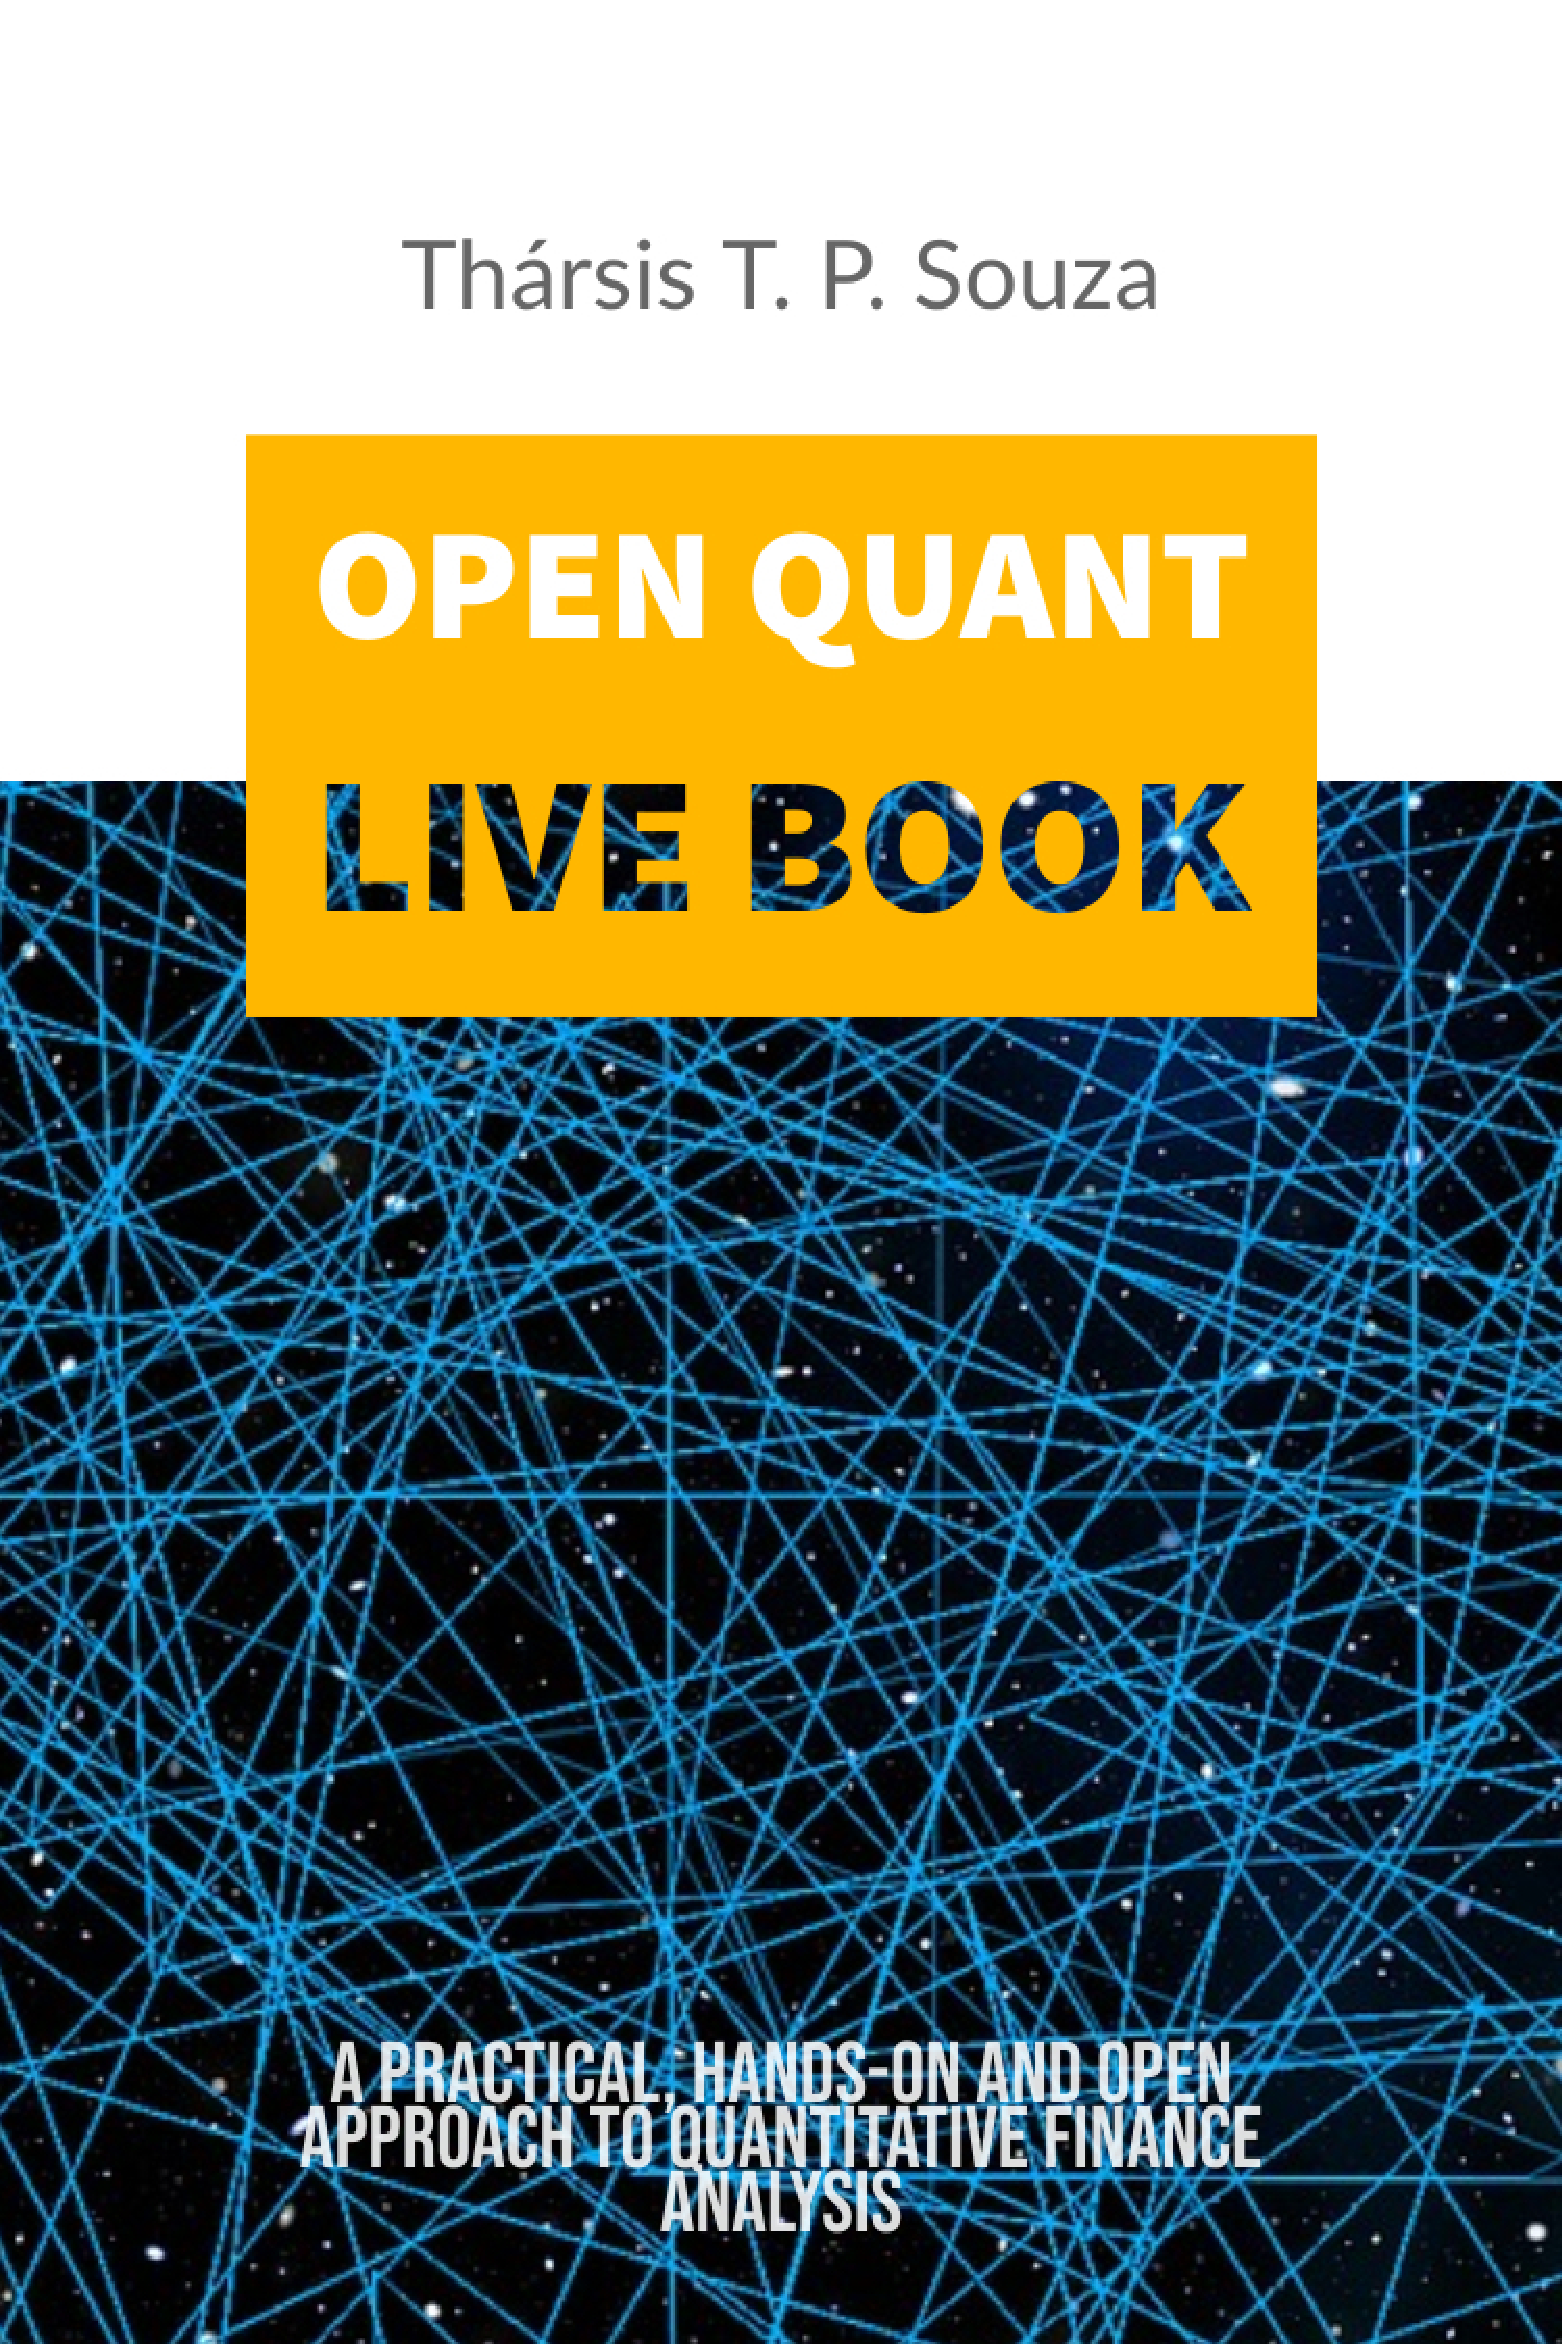
\includepdf{./fig/cover1.pdf}

\maketitle

{
\hypersetup{linkcolor=}
\setcounter{tocdepth}{2}
\tableofcontents
}
\newcommand{\independent}{\perp\!\!\!\!\perp}

\DeclarePairedDelimiter\ceil{\lceil}{\rceil}
\DeclarePairedDelimiter\floor{\lfloor}{\rfloor}

\chapter*{Preface}\label{preface}


\subsection*{Description}\label{description}


The book aims to be an Open Source introductory reference of the most
important aspects of financial data analysis, algo trading, portfolio
selection, econophysics and machine learning in finance with an emphasis
in reproducibility and openness not to be found in most other typical
Wall Street-like references.

\subsection*{Contribute}\label{contribute}


The Book is Open and we welcome co-authors. Feel free to
\href{https://www.openquants.com/contact}{reach out} or simply create a
pull request with your contribution! See project structure, guidelines
and how to contribute
\href{https://github.com/souzatharsis/open-quant-live-book/blob/master/CONTRIBUTING.md}{here}.

\subsection*{Working Contents}\label{working-contents}


\begin{enumerate}
\def\labelenumi{\arabic{enumi}.}
\tightlist
\item
  The Basics
\end{enumerate}

\begin{itemize}
\tightlist
\item
  I/O
\item
  Stylized Facts
\end{itemize}

\begin{enumerate}
\def\labelenumi{\arabic{enumi}.}
\setcounter{enumi}{1}
\tightlist
\item
  Algo Trading
\end{enumerate}

\begin{itemize}
\tightlist
\item
  Investment Process
\item
  Backtesting
\item
  Factor Investing
\item
  Limit Order
\end{itemize}

\begin{enumerate}
\def\labelenumi{\arabic{enumi}.}
\setcounter{enumi}{2}
\tightlist
\item
  Portfolio Optimization
\end{enumerate}

\begin{itemize}
\tightlist
\item
  Convex Optimization
\item
  Risk Parity Portfolios
\end{itemize}

\begin{enumerate}
\def\labelenumi{\arabic{enumi}.}
\setcounter{enumi}{3}
\tightlist
\item
  Machine Learning
\end{enumerate}

\begin{itemize}
\tightlist
\item
  Intro
\item
  Agent-Based Models
\item
  Binary Classifiers
\item
  AutoML
\item
  Hierarchical Risk Parity
\end{itemize}

\begin{enumerate}
\def\labelenumi{\arabic{enumi}.}
\setcounter{enumi}{4}
\tightlist
\item
  Econophysics
\end{enumerate}

\begin{itemize}
\tightlist
\item
  Entropy, Efficiency and Bubbles
\item
  Nonparametric Statistical Causality: An Information-Theoretical
  Approach
\item
  Financial Networks
\end{itemize}

\begin{enumerate}
\def\labelenumi{\arabic{enumi}.}
\setcounter{enumi}{5}
\tightlist
\item
  Alternative Data
\end{enumerate}

\begin{itemize}
\tightlist
\item
  The Market, The Players, The Rules
\item
  Case Studies
\end{itemize}

\subsection*{Book's information}\label{books-information}


First published at: \href{https://openquants.com/}{openquants.com}.

Licensed under
\href{https://creativecommons.org/licenses/by-nc-sa/4.0/}{Attribution-NonCommercial-ShareAlike
4.0 International}.

\begin{center}
\includegraphics[width=0.15\linewidth]{fig/by-nc-sa} \end{center}

\BeginKnitrBlock{flushright}
Copyright (c) 2019. OpenQuants.com, New York, NY.
\EndKnitrBlock{flushright} \BeginKnitrBlock{flushright}

\href{http://patreon.com/openquants}{
\includegraphics{https://github.com/souzatharsis/open-quant-live-book/blob/master/fig/patreon.png}}
\EndKnitrBlock{flushright}

\part{The Basics}\label{part-the-basics}

\chapter{I/O}\label{io}

In this Chapter, we will introduce basic functions to read text, excel
and JSON files as well as large files.

We will also show how to obtain free financial and economic data
including the following:

\begin{itemize}
\tightlist
\item
  End-of-day and real-time pricing;
\item
  Company financials;
\item
  Macroeconomic data.
\end{itemize}

Data sources utilized in this Chapter include the following:

\begin{itemize}
\tightlist
\item
  U.S. Securities and Exchange Commission;
\item
  Quandl;
\item
  IEX;
\item
  Alpha Vantage.
\end{itemize}

\section{Importing Data}\label{importing-data}

\subsection{Text Files}\label{text-files}

The most basic and commonly used option to import data from text files
in R is the use of the function \texttt{read.table} from the
\textbf{r-base}. We can use this function to read text files with
extensions such as \texttt{.txt} and \texttt{.csv}.

\begin{Shaded}
\begin{Highlighting}[]
\NormalTok{dat.table <-}\StringTok{ }\KeywordTok{read.table}\NormalTok{(}\DataTypeTok{file =} \StringTok{"<name of your file>.txt"}\NormalTok{)}
\NormalTok{dat.csv <-}\StringTok{ }\KeywordTok{read.csv}\NormalTok{(}\DataTypeTok{file =} \StringTok{"<name of your file>.csv"}\NormalTok{)}
\end{Highlighting}
\end{Shaded}

The package \textbf{readr} provides functions for reading text data into
R that are much faster that the functions from the \textbf{r-base}. The
\texttt{read\_table} function from the package \textbf{readr} provides a
near-replacement for the \texttt{read.table} function.

\begin{Shaded}
\begin{Highlighting}[]
\KeywordTok{library}\NormalTok{(readr)}
\NormalTok{dat.table <-}\StringTok{ }\NormalTok{readr}\OperatorTok{::}\KeywordTok{read_table2}\NormalTok{(}\DataTypeTok{file =} \StringTok{"<name of your file>.txt"}\NormalTok{)}
\NormalTok{dat.csv <-}\StringTok{ }\NormalTok{readr}\OperatorTok{::}\KeywordTok{read_csv}\NormalTok{(}\DataTypeTok{file =} \StringTok{"<name of your file>.csv"}\NormalTok{)}
\end{Highlighting}
\end{Shaded}

Another option to save data is to write it in \texttt{rds} format. Data
stored in \texttt{rds} format has the advantage to keep the original
data struture and type of the object saved. Also, \texttt{.rds} files
are compressed and consume less space than files saved in \texttt{.csv}
format. A data.frame object can be saved in \texttt{rds} format and then
loaded back as follows:

\begin{Shaded}
\begin{Highlighting}[]
\KeywordTok{write_rds}\NormalTok{(dat.frame, }\DataTypeTok{path =} \StringTok{"<name of your file>.rds"}\NormalTok{)}
\NormalTok{dat.frame <-}\StringTok{ }\KeywordTok{read_rds}\NormalTok{(}\DataTypeTok{path =} \StringTok{"<name of your file>.rds"}\NormalTok{)}
\end{Highlighting}
\end{Shaded}

\subsection{Excel Files}\label{excel-files}

The package \texttt{readxl} has an ease to use interface to functions
that load excel documents in R. The functions \texttt{read\_xls} and
\texttt{read\_xlsx} can be used to read excel files as follows:

\begin{Shaded}
\begin{Highlighting}[]
\KeywordTok{library}\NormalTok{(readxl)}
\NormalTok{readxl}\OperatorTok{::}\KeywordTok{read_xls}\NormalTok{(}\DataTypeTok{path =} \StringTok{"<name of your file>.xls"}\NormalTok{)}
\NormalTok{readxl}\OperatorTok{::}\KeywordTok{read_xlsx}\NormalTok{(}\DataTypeTok{path =} \StringTok{"<name of your file>.xlsx"}\NormalTok{)}
\end{Highlighting}
\end{Shaded}

The function \texttt{read\_excel()} automatically detects the extension
of the input file as follows:

\begin{Shaded}
\begin{Highlighting}[]
\NormalTok{readxl}\OperatorTok{::}\KeywordTok{read_excel}\NormalTok{(}\StringTok{"<name and extension of your file>"}\NormalTok{, }\DataTypeTok{sheet =} \StringTok{"<sheet name or index>"}\NormalTok{)}
\end{Highlighting}
\end{Shaded}

In the \texttt{read\_excel} function, the \texttt{sheet} argument can
receive either the target sheet name or index number, where sheet
indexing starts at 1.

The \texttt{readxl} has been oberving increased use compared to other
comparable packages such as \textbf{gdata} and the \textbf{xlsx} due to
its relative ease of use and performance. Also, the \texttt{readxl} do
not have depency with external code libraries while the packages
\textbf{gdata} and \textbf{xlsx} depend on \texttt{ActiveState\ PERL}
and the \texttt{Java\ JDK}, respectively.

\subsection{JSON Files}\label{json-files}

JSON files are particularly used for transmitting data in web
applications but also frequently used as a standard data interchange
format.

The \texttt{jsonline} package can be used to parse files in JSON format
as follows:

\begin{Shaded}
\begin{Highlighting}[]
\KeywordTok{library}\NormalTok{(jsonlite)}
\NormalTok{result_json <-}\StringTok{ }\KeywordTok{read_json}\NormalTok{(}\StringTok{"<json file>"}\NormalTok{)}
\end{Highlighting}
\end{Shaded}

\subsection{Large Files}\label{large-files}

Fast data manipulation in a short and flexible syntax.

\section{Data Sources}\label{data-sources}

In this section, we will show how to obtain financial and economic data
from public sources.

\subsection{Alpha Vantage}\label{alpha-vantage}

Alpha Vantage offers free access to pricing data including:

\begin{itemize}
\tightlist
\item
  Stock Time Series Data;
\item
  Physical and Digital/Crypto Currencies (e.g., Bitcoin);
\item
  Technical Indicators and
\item
  Sector Performances.
\end{itemize}

The data are available in JSON and CSV formats via REST APIs. The
\textbf{quantmod} and the \textbf{alphavantager} R packages offer a
lightweight R interface to the Alpha Vantage API. Daily stock prices can
be obtained with the \texttt{quantmod::getSymbols} function as follows:

\begin{Shaded}
\begin{Highlighting}[]
\KeywordTok{getSymbols}\NormalTok{(}\DataTypeTok{Symbols =} \StringTok{"AAPL"}\NormalTok{, }\DataTypeTok{src =} \StringTok{"av"}\NormalTok{, }\DataTypeTok{output.size =} \StringTok{"full"}\NormalTok{, }
  \DataTypeTok{adjusted =} \OtherTok{TRUE}\NormalTok{, }\DataTypeTok{api.key =} \StringTok{"your API key"}\NormalTok{)}
\end{Highlighting}
\end{Shaded}

The output data is stored in an object with the same name as the
corresponding symbol, in this example \texttt{AAPL}. The output data
looks like the following

\begin{tabular}{rrrrrr}
\toprule
AAPL.Open & AAPL.High & AAPL.Low & AAPL.Close & AAPL.Volume & AAPL.Adjusted\\
\midrule
102.4 & 102.5 & 98.9 & 99.0 & 4731800 & 3.08\\
98.4 & 99.8 & 94.8 & 94.9 & 3891700 & 2.95\\
93.2 & 97.2 & 91.1 & 97.0 & 5562300 & 3.01\\
98.0 & 98.4 & 94.0 & 98.3 & 4141300 & 3.05\\
100.9 & 102.0 & 98.5 & 100.0 & 4419700 & 3.11\\
\addlinespace
99.6 & 99.6 & 96.6 & 98.0 & 2535600 & 3.04\\
\bottomrule
\end{tabular}

\begin{center}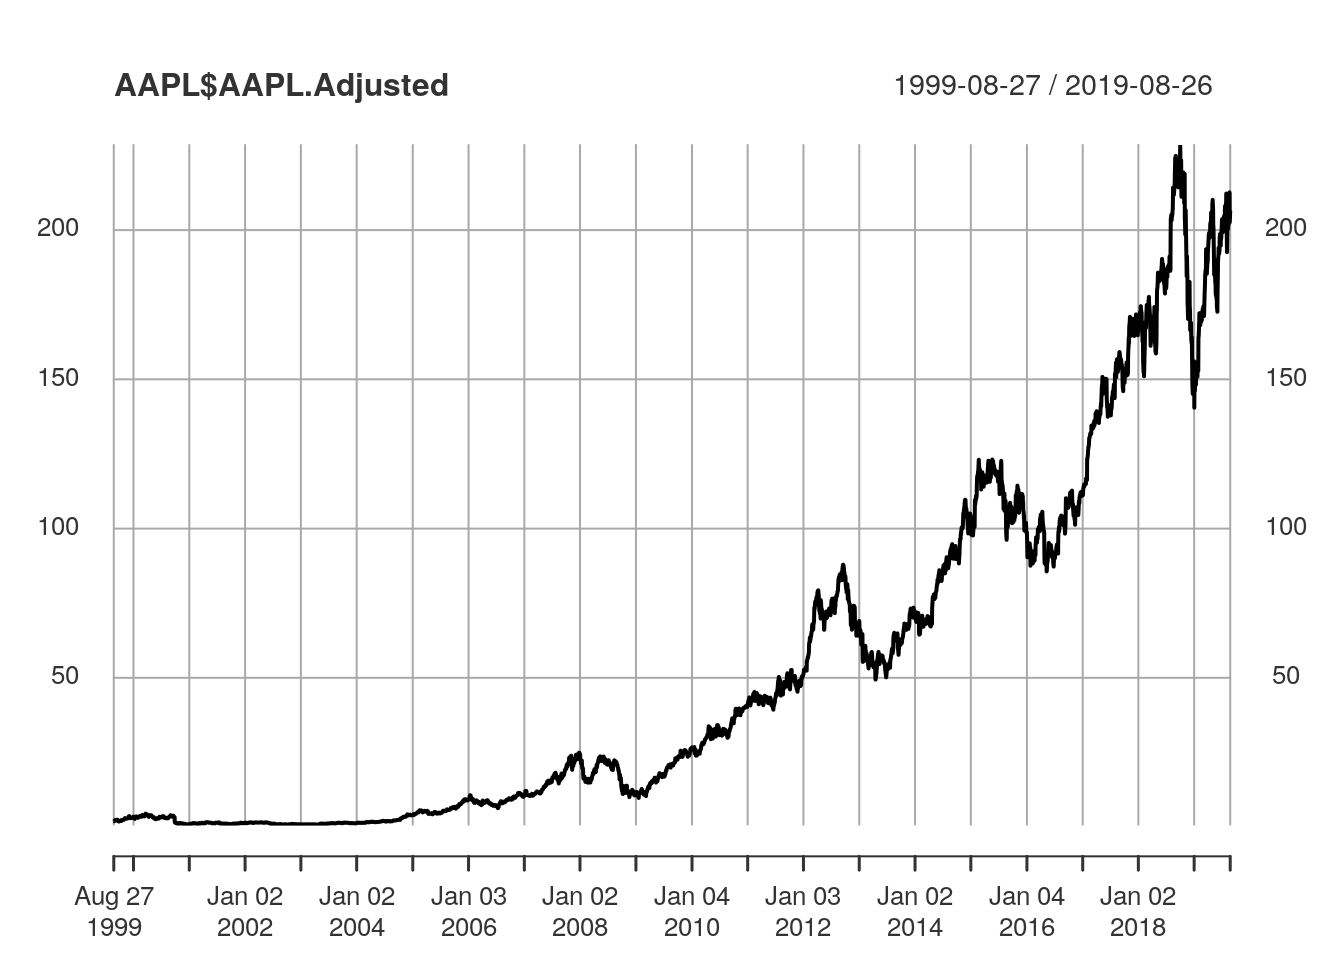
\includegraphics{open-quant-live-book_files/figure-latex/unnamed-chunk-16-1} \end{center}

We called the \texttt{quantmod::getSymbols} function with the following
arguments:

\begin{itemize}
\tightlist
\item
  \texttt{Symbols=\textquotesingle{}AAPL\textquotesingle{}} defines a
  character vector specifying the names of each symbol to be loaded,
  here specified by the symbol of the company Apple Inc.;
\item
  \texttt{src="av"} specifies the sourcing method, here defined with the
  value corresponding to Alpha Vantage;
\item
  \texttt{output.size="full"}specified length of the time series
  returned. The strings \texttt{compact} and \texttt{full} are accepted
  with the following specifications: \texttt{compact} returns only the
  latest 100 data points; \texttt{full} returns the full-length time
  series of up to 20 years of historical data;
\item
  \texttt{adjusted=TRUE} defines a boolean variable to include a column
  of closing prices adjusted for dividends and splits;
\item
  \texttt{api.key} specifies your Alpha Vantage API key.
\end{itemize}

\subsection{IEX}\label{iex}

The IEX Group operates the Investors Exchange (IEX), a stock exchange
for U.S. equities that is built for investors and companies. IEX offers
U.S. reference and market data including end-of-day and intraday pricing
data. IEX offers an API with ``a set of services designed for developers
and engineers. It can be used to build high-quality apps and services''.
Data sourced from the IEX API is freely available for commercial subject
to \href{https://iextrading.com/api-exhibit-a/}{conditions} and the use
of their API is subject to additional
\href{https://iextrading.com/api-terms/}{terms of use}.

IEX lists the following github project as an unofficial API for R:
\url{https://github.com/imanuelcostigan/iex}. We will provide examples
on how to obtain intraday pricing data using this package. First, we
will use the \textbf{devtools} to install the package directly from its
github repository as follows:

\begin{Shaded}
\begin{Highlighting}[]
\KeywordTok{library}\NormalTok{(devtools)}
\KeywordTok{install_github}\NormalTok{(}\StringTok{"imanuelcostigan/iex"}\NormalTok{)}
\end{Highlighting}
\end{Shaded}

The \textbf{iex} package provides 4 set of functions as follows:

\begin{itemize}
\tightlist
\item
  \texttt{last}: Provides IEX near real time last sale price, size and
  time. Last is ideal for developers that need a lightweight stock
  quote. \href{https://iextrading.com/developer/docs/\#last}{IEX API
  real time API documentation}.
\item
  \texttt{market}: Provides exchange trade volume data in near real
  time. \href{https://iextrading.com/developer/\#market-market}{IEX
  market API documentation}.
\item
  \texttt{stats}: A set of functions that return trading statistics.
  \href{https://iextrading.com/developer/\#stats}{IEX stats API
  documentation}.
\item
  \texttt{tops}: Provides IEX's aggregated bid and offer position in
  near real time for all securities on IEX's displayed limit order book.
  \href{https://iextrading.com/developer/\#tops-tops}{IEX API TOPS
  documentation}.
\end{itemize}

For instance, the \texttt{last} function has the following arguments:

\begin{itemize}
\tightlist
\item
  \texttt{symbols}: A vector of tickers (case insensitive). Special
  characters will be escaped. A list of eligible symbols is
  \href{https://iextrading.com/trading/eligible-symbols/}{published
  daily} by the IEX. When set to \texttt{NULL} (default) returns values
  for all symbols.
\item
  \texttt{fields}: A vector of fields names to return (case sensitive).
  When set to \texttt{NULL} (default) returns values for all fields.
\item
  \texttt{version}: The API version number, which is used to define the
  API URL.
\end{itemize}

We can obtain intraday stock price data with the \texttt{last} function
as follows:

\begin{Shaded}
\begin{Highlighting}[]
\NormalTok{dat <-}\StringTok{ }\NormalTok{iex}\OperatorTok{::}\KeywordTok{last}\NormalTok{(}\DataTypeTok{symbols =} \KeywordTok{c}\NormalTok{(}\StringTok{"AAPL"}\NormalTok{), }\DataTypeTok{fields =} \KeywordTok{c}\NormalTok{(}\StringTok{"symbol"}\NormalTok{, }
  \StringTok{"price"}\NormalTok{, }\StringTok{"size"}\NormalTok{))}
\end{Highlighting}
\end{Shaded}

The function returns an S3 object of class \texttt{iex\_api} which has
three accessible fields: \texttt{path} , \texttt{response} and
\texttt{content}.

\begin{itemize}
\tightlist
\item
  The \texttt{path} contains the corresponding IEX API path:
\end{itemize}

\begin{Shaded}
\begin{Highlighting}[]
\NormalTok{dat}\OperatorTok{$}\NormalTok{path}
\end{Highlighting}
\end{Shaded}

\begin{verbatim}
## [1] "tops/last"
\end{verbatim}

\begin{itemize}
\tightlist
\item
  The \texttt{response} contains the unparsed IEX API response:
\end{itemize}

\begin{Shaded}
\begin{Highlighting}[]
\NormalTok{dat}\OperatorTok{$}\NormalTok{response}
\end{Highlighting}
\end{Shaded}

\begin{verbatim}
## Response [https://api.iextrading.com/1.0/tops/last?symbols=AAPL&filter=symbol%2Cprice%2Csize]
##   Date: 2019-12-16 03:01
##   Status: 200
##   Content-Type: application/json; charset=utf-8
##   Size: 44 B
\end{verbatim}

\begin{itemize}
\tightlist
\item
  The \texttt{content} contains the parsed content from the API's
  response:
\end{itemize}

\begin{Shaded}
\begin{Highlighting}[]
\NormalTok{dat}\OperatorTok{$}\NormalTok{content}
\end{Highlighting}
\end{Shaded}

\begin{verbatim}
## [[1]]
## [[1]]$symbol
## [1] "AAPL"
## 
## [[1]]$price
## [1] 275
## 
## [[1]]$size
## [1] 52
\end{verbatim}

According to the developer, this package causes R to pause 0.2 seconds
after executing an API call to avoid the user being throttled by the IEX
API (which enforces a 5 request per second limit). Documentation about
the other set of functions can be obtained at
\url{https://github.com/imanuelcostigan/iex/tree/master/man}.

\subsection{Quandl}\label{quandl}

\href{https://www.quandl.com}{\textbf{Quandl}} is likely the largest
financial and alternative data aggregator/provider today. They leverage
relationships with third-party providers to be a one-stop-shop for
alternative data and traditional fundamental, pricing and estimates
datasets.

Quandl offer an API which usage is free for registered users. You can
obtain an API key
\href{https://www.quandl.com/sign-up-modal?defaultModal=showSignUp}{here}.
After signing up, just append your API key to your call like this:

\begin{verbatim}
https://www.quandl.com/api/v3/datasets/WIKI/FB/data.csv?api_key=YOURAPIKEYHERE
\end{verbatim}

At Quandl, every dataset is identified by ``Quandl code'', which is a
unique id. In the above example, you downloaded a dataset with the
Quandl code ``WIKI/FB''.

Every Quandl code has 2 parts: the database code (``WIKI'') which
specifies where the data comes from, and the dataset code (``FB'') which
identifies the specific time series you want.

You can find Quandl codes using their
\href{https://www.quandl.com/search}{data browser}. Additional API
documentation can be found \href{https://docs.quandl.com/}{here}.

Quandl is also available via an R interface \citep{R-Quandl}. For
instance, we can obtain Crude Oil Futures prices from 01/01/2010 to
01/01/2019 as follows:

\begin{Shaded}
\begin{Highlighting}[]
\KeywordTok{library}\NormalTok{(Quandl)}
\KeywordTok{Quandl.api_key}\NormalTok{(config}\OperatorTok{::}\KeywordTok{get}\NormalTok{()}\OperatorTok{$}\NormalTok{quandl.key)}
\NormalTok{from.dat <-}\StringTok{ }\KeywordTok{as.Date}\NormalTok{(}\StringTok{"01/01/2010"}\NormalTok{, }\DataTypeTok{format =} \StringTok{"%d/%m/%Y"}\NormalTok{)}
\NormalTok{to.dat <-}\StringTok{ }\KeywordTok{as.Date}\NormalTok{(}\StringTok{"01/01/2019"}\NormalTok{, }\DataTypeTok{format =} \StringTok{"%d/%m/%Y"}\NormalTok{)}
\NormalTok{crude.oil.futures <-}\StringTok{ }\KeywordTok{Quandl}\NormalTok{(}\StringTok{"CHRIS/CME_CL1"}\NormalTok{, }\DataTypeTok{start_date =}\NormalTok{ from.dat, }
  \DataTypeTok{end_date =}\NormalTok{ to.dat, }\DataTypeTok{type =} \StringTok{"xts"}\NormalTok{)}
\KeywordTok{plot}\NormalTok{(crude.oil.futures}\OperatorTok{$}\NormalTok{Last)}
\end{Highlighting}
\end{Shaded}

\begin{center}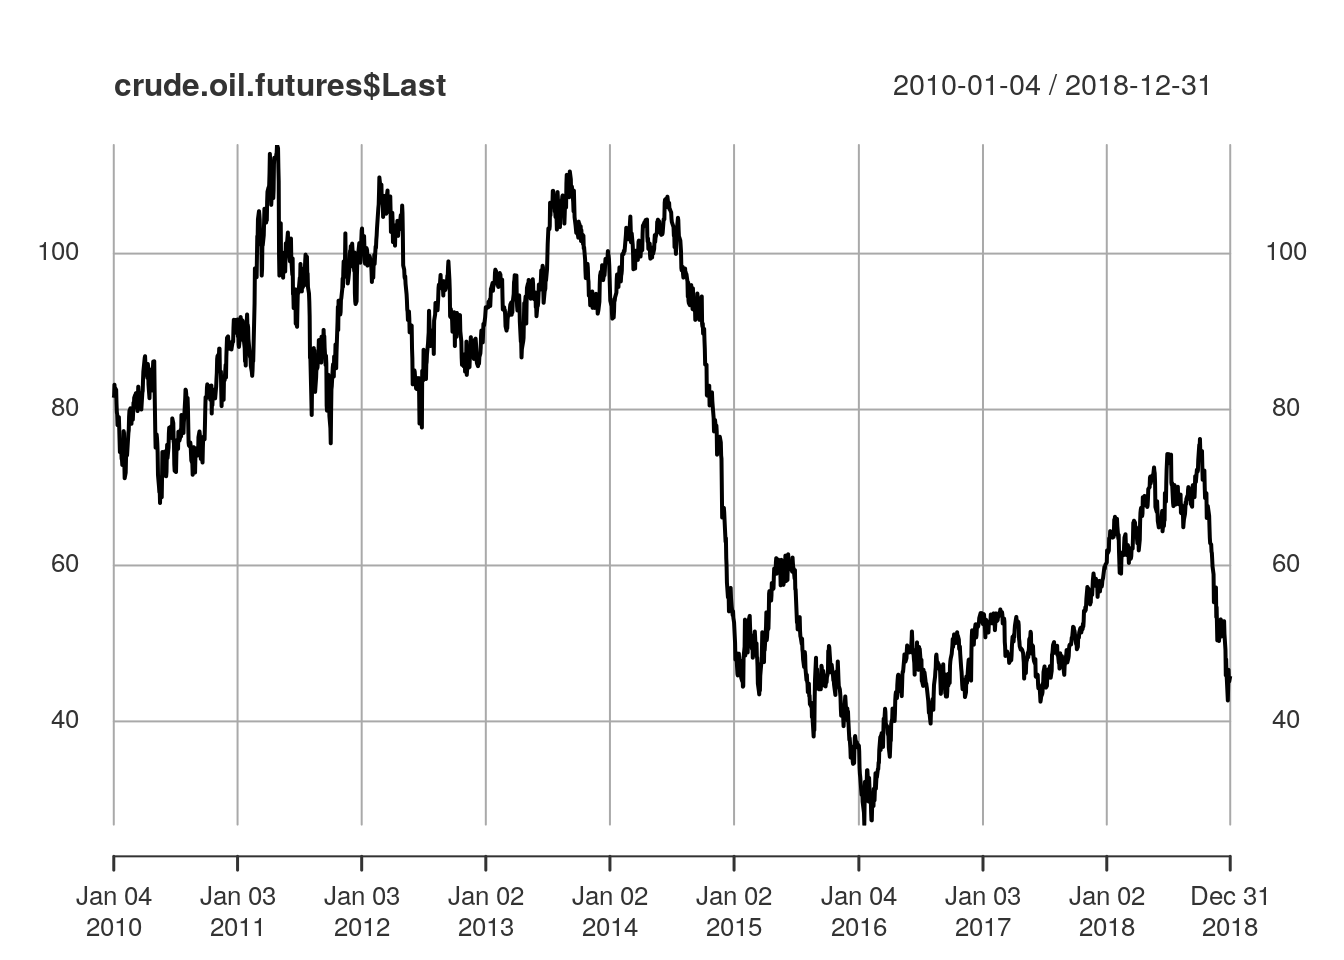
\includegraphics{open-quant-live-book_files/figure-latex/unnamed-chunk-22-1} \end{center}

In the example above we specified the following Database/Dataset:

\begin{itemize}
\tightlist
\item
  Database: ``CHRIS''. Continuous contracts for all 600 futures on
  Quandl. Built on top of raw data from CME, ICE, LIFFE etc. Curated by
  the Quandl community. 50 years history.
\item
  Dataset: ``CME\_CL1''. Historical futures prices of Crude Oil Futures,
  Continuous Contract \#1. Non-adjusted price based on spot-month
  continuous contract calculations. Raw data from CME.
\end{itemize}

\subsection{SEC}\label{sec}

Official filings are freely available from the U.S. Securities and
Exchange Commission's EDGAR database. The package \texttt{finreportr}
provides an interface in R to facilitate financial analysis from SEC's
10K and 10K/A filings.

We can obtain company basic information with the function the
\texttt{CompanyInfo} function by passing the ticker symbol of the target
company as follows:

\begin{Shaded}
\begin{Highlighting}[]
\KeywordTok{library}\NormalTok{(}\StringTok{"finreportr"}\NormalTok{)}
\NormalTok{AAPL.Info <-}\StringTok{ }\KeywordTok{CompanyInfo}\NormalTok{(}\StringTok{"AAPL"}\NormalTok{)}
\KeywordTok{print}\NormalTok{(AAPL.Info)}
\end{Highlighting}
\end{Shaded}

\begin{verbatim}
##      company        CIK  SIC state state.inc FY.end
## 1 Apple Inc. 0000320193 3571    CA        CA   0928
##       street.address         city.state
## 1 ONE APPLE PARK WAY CUPERTINO CA 95014
\end{verbatim}

As a result, we obtain the following information:

\begin{itemize}
\tightlist
\item
  Company name: Apple Inc.;
\item
  SEC Central Index Key (CIK): 0000320193;
\item
  Standard Industrial Classification (SIC): 3571, which is the industry
  code for Electronic Computers;
\item
  Address: ONE APPLE PARK WAY, CUPERTINO CA 95014;
\item
  Most recent period of report end is 0928.
\end{itemize}

The list of company annual reports with corresponding filing dates can
be obtained with the function \emph{AnnualReports} as follows:

\begin{Shaded}
\begin{Highlighting}[]
\NormalTok{AAPL.reports <-}\StringTok{ }\KeywordTok{AnnualReports}\NormalTok{(}\StringTok{"AAPL"}\NormalTok{)}
\end{Highlighting}
\end{Shaded}

\begin{table}[t]

\caption{\label{tab:unnamed-chunk-25}Sample Annual Reports}
\centering
\begin{tabular}{lll}
\toprule
filing.name & filing.date & accession.no\\
\midrule
10-K & 2019-10-31 & 0000320193-19-000119\\
10-K & 2018-11-05 & 0000320193-18-000145\\
10-K & 2017-11-03 & 0000320193-17-000070\\
10-K & 2016-10-26 & 0001628280-16-020309\\
10-K & 2015-10-28 & 0001193125-15-356351\\
\addlinespace
10-K & 2014-10-27 & 0001193125-14-383437\\
\bottomrule
\end{tabular}
\end{table}

The accession number is a unique identifier that the SEC creates for
each filing.

Company financials are organized into 3 segments: Income Statement,
Balance Sheet and Cash Flow.

\textbf{Income Statement}

Financials from the Income Statement segment can be obtained with the
\emph{GetIncome} function as follows:

\begin{Shaded}
\begin{Highlighting}[]
\NormalTok{AAPL.IS <-}\StringTok{ }\KeywordTok{GetIncome}\NormalTok{(}\StringTok{"AAPL"}\NormalTok{, }\DecValTok{2017}\NormalTok{)}
\end{Highlighting}
\end{Shaded}

\begin{table}[t]

\caption{\label{tab:unnamed-chunk-28}Sample Income Statement Financials}
\centering
\begin{tabular}{lllll}
\toprule
Metric & Units & Amount & startDate & endDate\\
\midrule
Revenue, Net & usd & 233715000000 & 2014-09-28 & 2015-09-26\\
Revenue, Net & usd & 75872000000 & 2015-09-27 & 2015-12-26\\
Revenue, Net & usd & 50557000000 & 2015-12-27 & 2016-03-26\\
Revenue, Net & usd & 42358000000 & 2016-03-27 & 2016-06-25\\
Revenue, Net & usd & 46852000000 & 2016-06-26 & 2016-09-24\\
\addlinespace
Revenue, Net & usd & 215639000000 & 2015-09-27 & 2016-09-24\\
\bottomrule
\end{tabular}
\end{table}

The Income Statement function returns data for the following metrics:

\begin{table}[t]

\caption{\label{tab:unnamed-chunk-29}Income Statement Metrics}
\centering
\begin{tabular}{l}
\toprule
Metrics\\
\midrule
Revenue, Net\\
Cost of Goods and Services Sold\\
Gross Profit\\
Research and Development Expense\\
Selling, General and Administrative Expense\\
\addlinespace
Operating Expenses\\
Operating Income (Loss)\\
Nonoperating Income (Expense)\\
Income (Loss) from Continuing Operations before Income Taxes, Noncontrolling Interest\\
Income Tax Expense (Benefit)\\
\addlinespace
Net Income (Loss) Attributable to Parent\\
Earnings Per Share, Basic\\
Earnings Per Share, Diluted\\
Weighted Average Number of Shares Outstanding, Basic\\
Weighted Average Number of Shares Outstanding, Diluted\\
\addlinespace
Common Stock, Dividends, Per Share, Declared\\
\bottomrule
\end{tabular}
\end{table}

\textbf{Balance Sheet}

Financials from the Balance Sheet segment can be obtained with the
\emph{GetBalanceSheet} function as follows:

\begin{Shaded}
\begin{Highlighting}[]
\NormalTok{AAPL.BS <-}\StringTok{ }\KeywordTok{GetBalanceSheet}\NormalTok{(}\StringTok{"AAPL"}\NormalTok{, }\DecValTok{2017}\NormalTok{)}
\end{Highlighting}
\end{Shaded}

\begin{table}[t]

\caption{\label{tab:unnamed-chunk-32}Sample Balance Sheet Financials}
\centering
\begin{tabular}{lllll}
\toprule
Metric & Units & Amount & startDate & endDate\\
\midrule
Cash and Cash Equivalents, at Carrying Value & usd & 13844000000 & NA & 2014-09-27\\
Cash and Cash Equivalents, at Carrying Value & usd & 21120000000 & NA & 2015-09-26\\
Cash and Cash Equivalents, at Carrying Value & usd & 20484000000 & NA & 2016-09-24\\
Cash and Cash Equivalents, at Carrying Value & usd & 20289000000 & NA & 2017-09-30\\
Available-for-sale Securities, Current & usd & 46671000000 & NA & 2016-09-24\\
\addlinespace
Available-for-sale Securities, Current & usd & 53892000000 & NA & 2017-09-30\\
\bottomrule
\end{tabular}
\end{table}

The Balance Sheet function returns data for the following metrics:

\begin{table}[t]

\caption{\label{tab:unnamed-chunk-33}Balance Sheet Metrics}
\centering
\begin{tabular}{l}
\toprule
Metrics\\
\midrule
Cash and Cash Equivalents, at Carrying Value\\
Available-for-sale Securities, Current\\
Accounts Receivable, Net, Current\\
Inventory, Net\\
Nontrade Receivables, Current\\
\addlinespace
Other Assets, Current\\
Assets, Current\\
Available-for-sale Securities, Noncurrent\\
Property, Plant and Equipment, Net\\
Goodwill\\
\addlinespace
Intangible Assets, Net (Excluding Goodwill)\\
Other Assets, Noncurrent\\
Assets\\
Accounts Payable, Current\\
Accrued Liabilities, Current\\
\addlinespace
Deferred Revenue, Current\\
Commercial Paper\\
Long-term Debt, Current Maturities\\
Liabilities, Current\\
Deferred Revenue, Noncurrent\\
\addlinespace
Long-term Debt, Excluding Current Maturities\\
Other Liabilities, Noncurrent\\
Liabilities\\
Commitments and Contingencies\\
Common Stocks, Including Additional Paid in Capital\\
\addlinespace
Retained Earnings (Accumulated Deficit)\\
Accumulated Other Comprehensive Income (Loss), Net of Tax\\
Stockholders' Equity Attributable to Parent\\
Liabilities and Equity\\
\bottomrule
\end{tabular}
\end{table}

\textbf{Cash Flow}

Financials from the Cash Flow segment can be obtained with the
\emph{GetCashFlow} function as follows:

\begin{Shaded}
\begin{Highlighting}[]
\NormalTok{AAPL.CF <-}\StringTok{ }\KeywordTok{GetCashFlow}\NormalTok{(}\StringTok{"AAPL"}\NormalTok{, }\DecValTok{2017}\NormalTok{)}
\end{Highlighting}
\end{Shaded}

\begin{table}[t]

\caption{\label{tab:unnamed-chunk-36}Sample Cash Flow Financials}
\centering
\begin{tabular}{lllll}
\toprule
Metric & Units & Amount & startDate & endDate\\
\midrule
Cash and Cash Equivalents, at Carrying Value & usd & 13844000000 & NA & 2014-09-27\\
Cash and Cash Equivalents, at Carrying Value & usd & 21120000000 & NA & 2015-09-26\\
Cash and Cash Equivalents, at Carrying Value & usd & 20484000000 & NA & 2016-09-24\\
Cash and Cash Equivalents, at Carrying Value & usd & 20289000000 & NA & 2017-09-30\\
Net Income (Loss) Attributable to Parent & usd & 53394000000 & 2014-09-28 & 2015-09-26\\
\addlinespace
Net Income (Loss) Attributable to Parent & usd & 18361000000 & 2015-09-27 & 2015-12-26\\
\bottomrule
\end{tabular}
\end{table}

The Cash Flow function returns data for the following metrics:

\begin{table}[t]

\caption{\label{tab:unnamed-chunk-37}Cash Flow Metrics}
\centering
\begin{tabular}{l}
\toprule
Metrics\\
\midrule
Cash and Cash Equivalents, at Carrying Value\\
Net Income (Loss) Attributable to Parent\\
Depreciation, Amortization and Accretion, Net\\
Share-based Compensation\\
Deferred Income Tax Expense (Benefit)\\
\addlinespace
Other Noncash Income (Expense)\\
Increase (Decrease) in Accounts Receivable\\
Increase (Decrease) in Inventories\\
Increase (Decrease) in Other Receivables\\
Increase (Decrease) in Other Operating Assets\\
\addlinespace
Increase (Decrease) in Accounts Payable\\
Increase (Decrease) in Deferred Revenue\\
Increase (Decrease) in Other Operating Liabilities\\
Net Cash Provided by (Used in) Operating Activities\\
Payments to Acquire Available-for-sale Securities\\
\addlinespace
Proceeds from Maturities, Prepayments and Calls of Available-for-sale Securities\\
Proceeds from Sale of Available-for-sale Securities\\
Payments to Acquire Businesses, Net of Cash Acquired\\
Payments to Acquire Property, Plant, and Equipment\\
Payments to Acquire Intangible Assets\\
\addlinespace
Payments to Acquire Other Investments\\
Payments for (Proceeds from) Other Investing Activities\\
Net Cash Provided by (Used in) Investing Activities\\
Proceeds from Issuance of Common Stock\\
Excess Tax Benefit from Share-based Compensation, Financing Activities\\
\addlinespace
Payments Related to Tax Withholding for Share-based Compensation\\
Payments of Dividends\\
Payments for Repurchase of Common Stock\\
Proceeds from Issuance of Long-term Debt\\
Repayments of Long-term Debt\\
\addlinespace
Proceeds from (Repayments of) Commercial Paper\\
Net Cash Provided by (Used in) Financing Activities\\
Cash and Cash Equivalents, Period Increase (Decrease)\\
Income Taxes Paid, Net\\
Interest Paid\\
\bottomrule
\end{tabular}
\end{table}

\section{Conclusion}\label{conclusion}

\begin{itemize}
\tightlist
\item
  We showed how to load and import data from both local files and
  external sources.
\item
  We provided examples on how to read tabular data and how to handle
  large files.
\item
  We showed how to obtain financial and economic data from freely
  available sources.
\end{itemize}

\subsection{Further Reading}\label{further-reading}

To further learn how to use R to load, transform, visualize and model
data see \citep{Wickham:2017:RDS:3086927}. Additional relevant R
packages include the following:

\begin{itemize}
\tightlist
\item
  dplyr: Fast data frames manipulation and database query.
\item
  reshape2: Flexibly rearrange, reshape and aggregate data.
\item
  readr: A fast and friendly way to read tabular data into R.
\item
  tidyr: Easily tidy data with spread and gather functions.
\item
  rlist: A toolbox for non-tabular data manipulation with lists.
\item
  jsonlite: A robust and quick way to parse JSON files in R.
\item
  ff: Data structures designed to store large datasets.
\item
  lubridate: A set of functions to work with dates and times.
\end{itemize}

\chapter{Stylized Facts}\label{stylized-facts}

\section{Introduction}\label{introduction}

\section{Distribution of Returns}\label{distribution-of-returns}

\subsection{Fat Tails}\label{fat-tails}

\subsection{Skewness}\label{skewness}

\section{Volatility}\label{volatility}

\subsection{Time-invariance}\label{time-invariance}

\subsection{Volatility Clustering}\label{volatility-clustering}

\subsection{Correlation with Trading
Volume}\label{correlation-with-trading-volume}

\section{Correlation}\label{correlation}

\subsection{Time-invariance}\label{time-invariance-1}

\subsection{Auto-correlation}\label{auto-correlation}

\part{Algo Trading}\label{part-algo-trading}

\part{Portfolio
Optimization}\label{part-portfolio-optimization}

\chapter{Risk Parity Portfolios}\label{risk-parity-portfolios}

\section{Introduction}\label{introduction-1}

The ``risk parity'' approach was popularized by Ray Dalio's Bridgewater
Associates - the largest hedge fund by assets under management (\$132.8
billions of USD) - with the creation of the All Weather asset allocation
strategy in 1996. ``All Weather'' is a term used to designate funds that
tend to perform reasonably well during both favorable and unfavorable
economic and market conditions. Today, several managers have employed
``All Weather'' concepts under a risk parity approach.

\begin{figure}[H]

{\centering 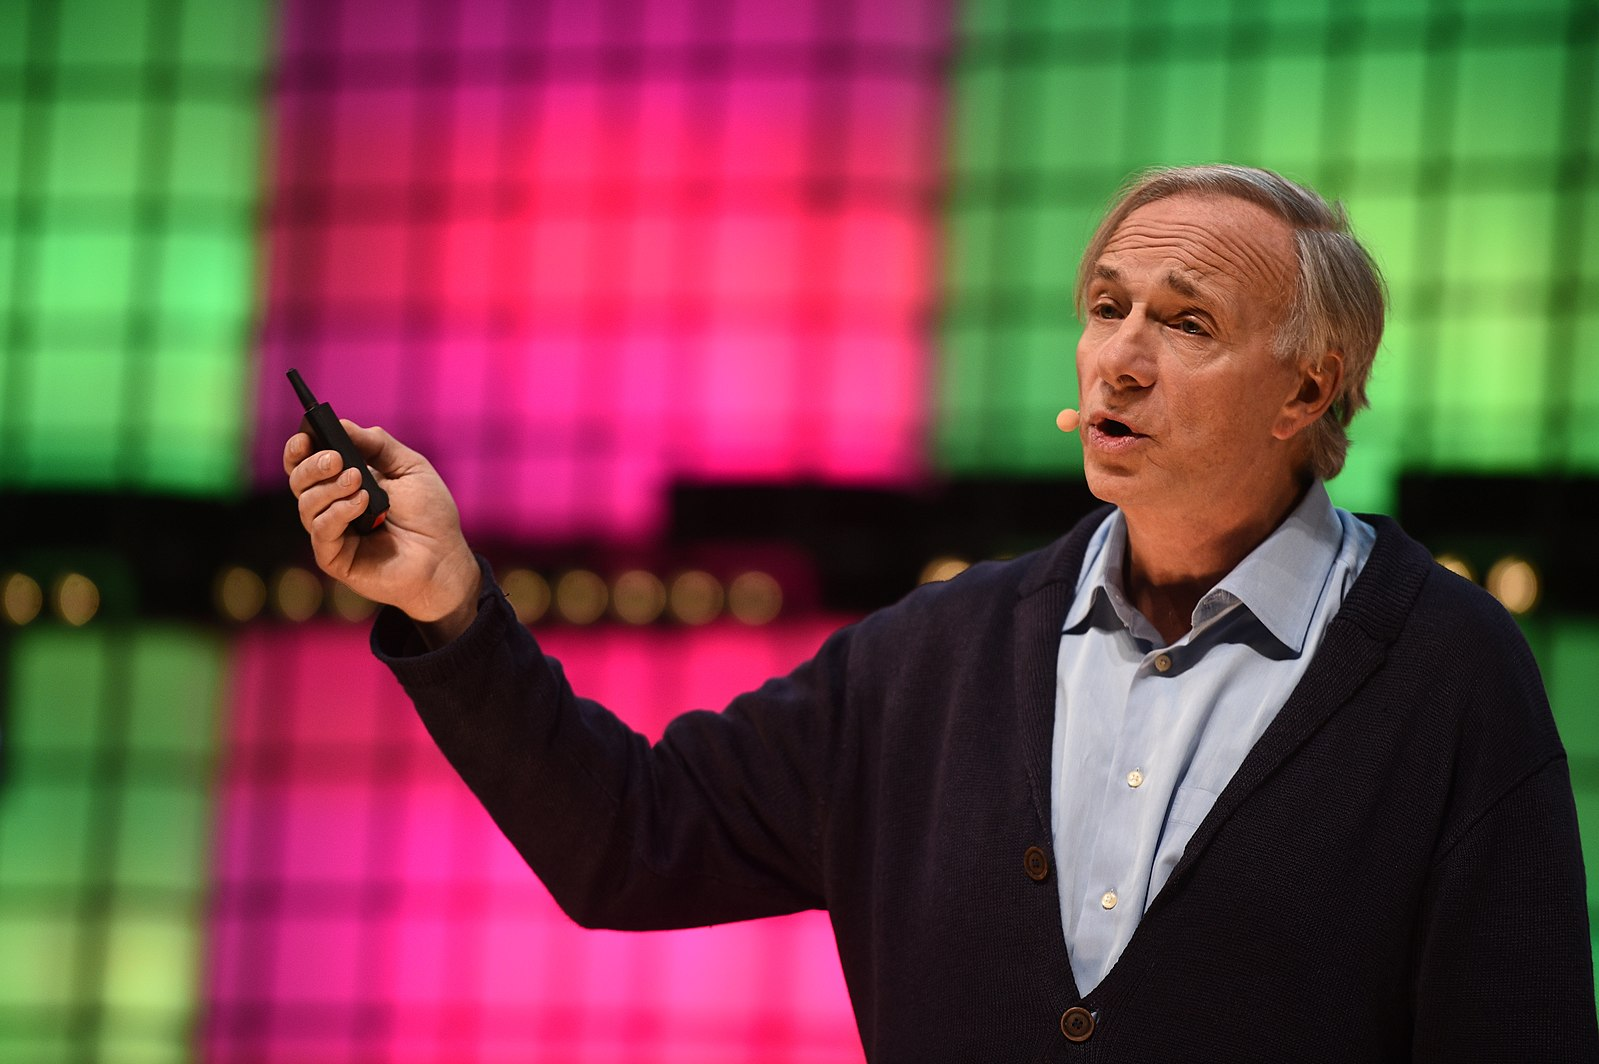
\includegraphics[width=1\linewidth]{./chapters/RiskParity/ray} 

}

\caption{7 November 2018; Ray Dalio, Bridgewater Associates on Centre Stage during day two of Web Summit 2018 at the Altice Arena in Lisbon, Portugal. Photo by David Fitzgerald/Web Summit via SportsfilePhoto by David Fitzgerald /Sportsfile.}\label{fig:unnamed-chunk-39}
\end{figure}

A risk parity portfolio seeks to achieve an equal balance between the
risk associated with each asset class or portfolio component. In that
way, lower risk asset classes will generally have higher notional
allocations than higher risk asset classes.

\begin{quote}
Risk Parity is about \textbf{Balance} -
\href{https://www.bridgewater.com}{Bridgewater}.
\end{quote}

Risk parity strategies suffered in recent history (2010-2017) as the
bull market has pushed stocks to a record high hence favoring
equity-concentrated portfolios. However, the increase in market
volatility since 2018, the emergency of geo-political and tradewars risk
as well as the growth in haven assets like Gold create conditions that
strengthen the case for diversified portfolios. This is demonstrated in
Fig. \ref{fig:riskparityBLO} which shows that the S\&P risk parity
strategy has returned almost 10\% over the last 12 months (Aug/2018 -
Aug-2019), more than double the S\&P 500 index of U.S. stocks.

\begin{figure}[H]

{\centering 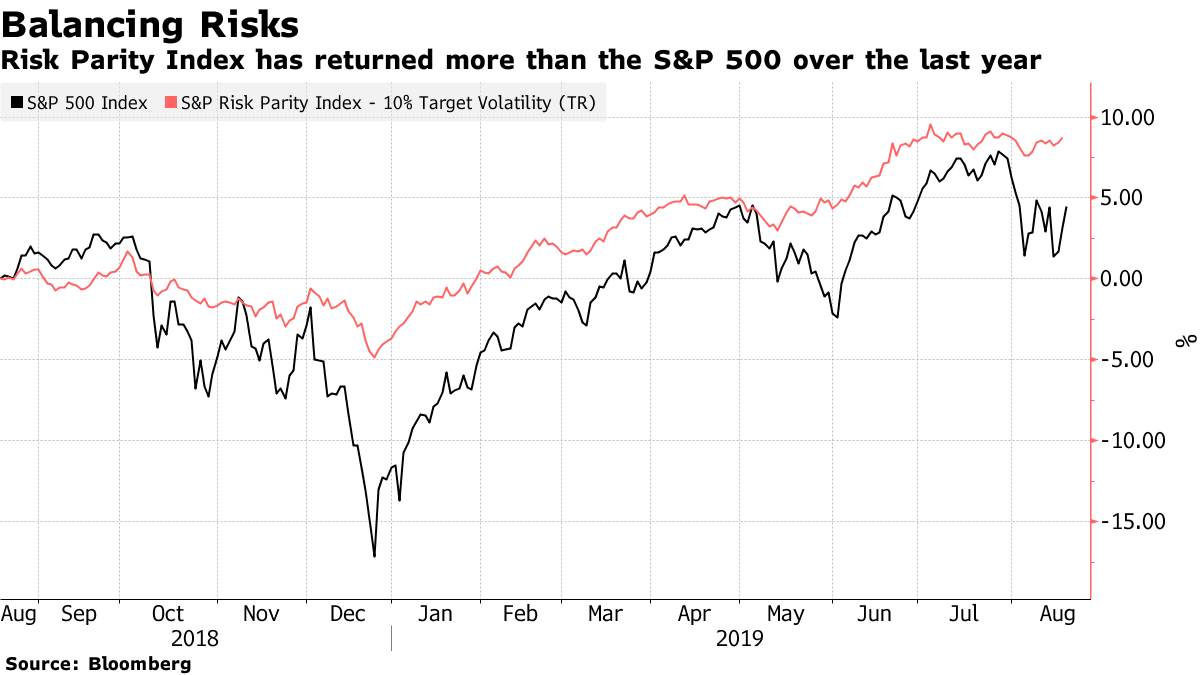
\includegraphics[width=1\linewidth]{./chapters/RiskParity/riskparity} 

}

\caption{S&P 500 index versus S&P Risk Parity Index. Source: Bloomberg.}\label{fig:riskparityBLO}
\end{figure}

In Aug/2019, there have been news about the launch of a new Risk Parity
ETF in the US. The RPAR Risk Parity ETF plans to allocate across asset
classes based on risk, regulatory filings show. The fund would be the
first in the U.S. to follow this quantitative approach, allotting more
money to securities with lower volatility according to
\href{https://www.bloomberg.com/news/articles/2019-08-19/ray-dalio-inspired-a-risk-parity-etf-by-bridgewater-bofa-alums}{Bloomberg}.

\begin{quote}
{[}The RPAR Risk Parity ETF is{]} kind of like Bridgewater does, but
they just do it for the wealthiest institutions in the world. The idea
here is to build something that would work for everybody. - Alex
Shahidi, former relationship manager at Dalio's Bridgewater Associate
and creator of the RPAR Risk Parity ETF.
\href{https://www.bloomberg.com/news/articles/2019-08-19/ray-dalio-inspired-a-risk-parity-etf-by-bridgewater-bofa-alums}{Bloomberg}.
\end{quote}

But how can we a risk parity portfolio? How does it perform against a
traditional mean/variance model?

In this Chapter,

\begin{enumerate}
\def\labelenumi{\arabic{enumi}.}
\tightlist
\item
  We will show how you can build your own Risk Parity portfolio
\item
  We will create and compare the performance two indices:
\end{enumerate}

\begin{itemize}
\tightlist
\item
  A FAANG Risk Parity Index of FAANG companies with equal risk balance
\item
  A FAANG Tangency Portfolio Index of FAANG companies with weights such
  that return/risk ratio is maximized
\end{itemize}

By the end of the Chapter, you will be able to create your own risk
parity / All Weather fund and compare it against your benchmark of
choice.

\section{Risk Parity Portfolio}\label{risk-parity-portfolio}

A risk parity portfolio denotes a class of portfolios whose assets
verify the following equalities \citep{R-riskParityPortfolio}:

\begin{equation}
w_{i} \frac{\partial f(\mathbf{w})}{\partial w_{i}}=w_{j} \frac{\partial f(\mathbf{w})}{\partial w_{j}}, \forall i, j
\end{equation}

where \(f\) is a positively homogeneous function of degree one that
measures the total risk of the portfolio and \(\mathbf{w}\) is the
portfolio weight vector. In other words, the marginal risk contributions
for every asset in a risk parity portfolio are equal. A common choice
for \(f\), for instance, is the standard deviation of the portfolio,
which is usually called volatility, i.e.,
\(f(\mathbf{w})=\sqrt{\mathbf{w}^{T} \mathbf{\Sigma} \mathbf{w}}\),
where \(\mathbf{\Sigma}\) is the covariance matrix of assets.

In practice, risk and portfolio managers have risk mandates they follow
or bounds for marginal risk contributions at the asset, country,
regional or sector levels. Hence, a natural extension of the risk parity
portfolio is the so called risk budget portfolio, in which the marginal
risk contributions match preassigned quantities
\citep{R-riskParityPortfolio}. Mathematically,

\begin{equation}
w_{i}(\Sigma \mathbf{w})_{i}=b_{i} \mathbf{w}^{T} \Sigma \mathbf{w}, \forall i,
\end{equation}

where
\(\mathbf{b} \triangleq\left(b_{1}, b_{2}, \ldots, b_{N}\right)\left(\text { with } \mathbf{1}^{T} \mathbf{b}=1 \text { and } \mathbf{b} \geq \mathbf{0}\right)\)
is the vector of desired marginal risk contributions.

\section{Tangency Portfolio}\label{tangency-portfolio}

Mean variance optimization is a commonly used quantitative tool part of
Modern Portfolio Theory that allows investors to perform allocation by
considering the trade-off between risk and return.

\begin{figure}[H]

{\centering 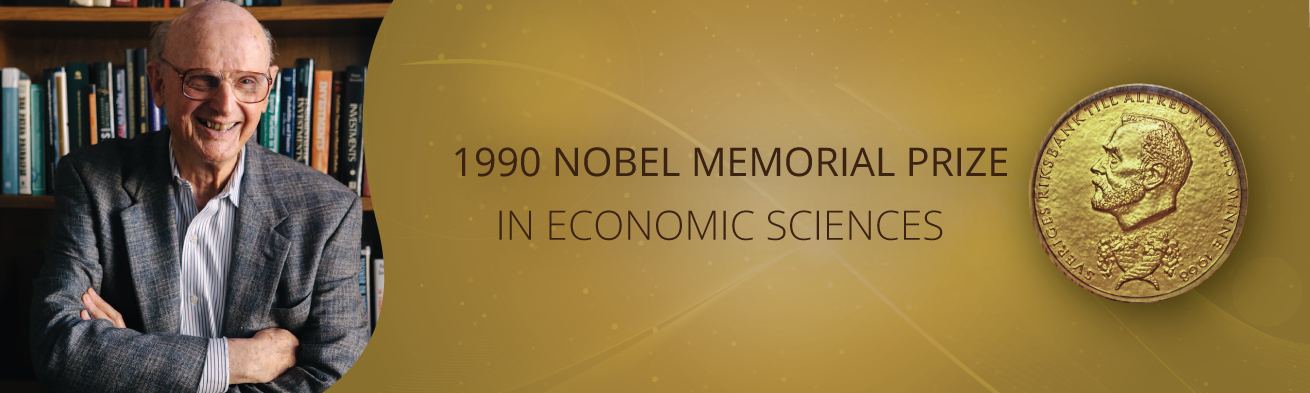
\includegraphics[width=1\linewidth]{./chapters/RiskParity/harry} 

}

\caption{In 1990, Dr. Harry M. Markowitz shared The Nobel Prize in Economics for his work on portfolio theory.}\label{fig:unnamed-chunk-40}
\end{figure}

In a mean-variance framework, the objective is to minimize portfolio
risk \(\sigma^2\) subject to a baseline expected rate of return
\(\mu_b\) as follows:

\begin{equation}
\begin{array}{ll}{\mathcal{M}} & {\text { minimize } \quad \frac{1}{2} w^{T} \Sigma w} \\ {\text { subject to }} & {\mathrm{m}^{T} w \geq \mu_{b}, \text { and } \mathbf{1}^{T} w=1}\end{array}
\end{equation}

where \(m\) is the vector of expected returns for the portfolio assets.

We will obtain an optimal portfolio (min risk) for each target rate of
return \(\mu_b\) thus forming an efficient frontier. Each point in the
efficient frontier in Fig. \ref{fig:efficientport} is a portfolio with
an optimal combination of securities that minimized risk given a level
of risk (standard deviation). The dots below the efficient frontier are
portfolios with inferior performance. They either offer the same returns
but with higher risk, or they offer less return for the same risk.

\begin{figure}[H]

{\centering 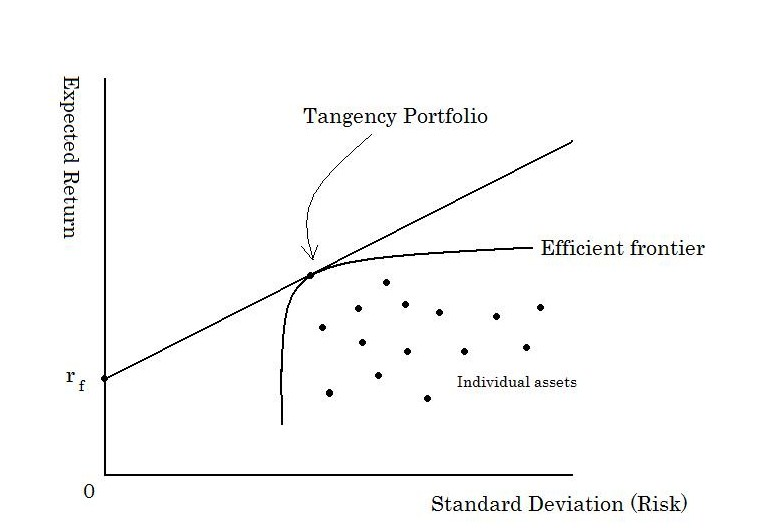
\includegraphics[width=1\linewidth]{./chapters/RiskParity/efficientport} 

}

\caption{Efficienty Frontier. Attribution: ShuBraque (CC BY-SA 3.0)}\label{fig:efficientport}
\end{figure}

But how can we choose a portfolio from the efficient frontier? One
approach is to choose the most efficient portfolio from a risk/return
standpoint, i.e., the portfolio with the highest Sharpe ratio (ratio
between excess return and portfolio standard deviation). This portfolio
is called the tangency portfolio and it's located at the tangency point
of the Capital Allocation Line and the Efficient Frontier.

We will implement both a parity risk and a tangency portfolio in the
next section.

\section{Optimizing FAANG: Ray Dalio versus
Markowitz}\label{optimizing-faang-ray-dalio-versus-markowitz}

\subsection{Single Portfolio}\label{single-portfolio}

First, we will load log-returns of adjusted prices for FAANG companies,
i.e., the stocks identified by the following tickers: FB, AMZN, AAPL,
NFLX and GOOG (see Appendix \ref{dt-FAANG} for code used to generate
this dataset).

\begin{Shaded}
\begin{Highlighting}[]
\KeywordTok{library}\NormalTok{(xts)}
\CommentTok{# load FAANG returns}
\NormalTok{faang.returns <-}\StringTok{ }\KeywordTok{as.xts}\NormalTok{(}\KeywordTok{read.zoo}\NormalTok{(}\StringTok{"./data/FAANG.csv"}\NormalTok{, }\DataTypeTok{header =} \OtherTok{TRUE}\NormalTok{, }
  \DataTypeTok{index.column =} \DecValTok{1}\NormalTok{, }\DataTypeTok{sep =} \StringTok{","}\NormalTok{))}
\end{Highlighting}
\end{Shaded}

We can use the packages \textbf{riskParityPortfolio} and
\textbf{fPortfolio} to build a FAANG risk parity and tangency
portfolios, respectively. We will first consider FAANG returns from 2018
to build the portfolios as follows:

\begin{Shaded}
\begin{Highlighting}[]
\KeywordTok{library}\NormalTok{(IDPmisc)}
\KeywordTok{library}\NormalTok{(riskParityPortfolio)}
\KeywordTok{library}\NormalTok{(fPortfolio)}

\CommentTok{# consider returns from 2018 omit days with missing data}
\CommentTok{# (INF/NA returns)}
\NormalTok{faang.returns.filtered <-}\StringTok{ }\KeywordTok{NaRV.omit}\NormalTok{(}\KeywordTok{as.matrix}\NormalTok{(faang.returns[}\StringTok{"2018"}\NormalTok{]))}

\CommentTok{# calculate covariance matrix}
\NormalTok{Sigma <-}\StringTok{ }\KeywordTok{cov}\NormalTok{(faang.returns.filtered)}

\CommentTok{# compute risk parity portfolio}
\NormalTok{portfolio.parity <-}\StringTok{ }\KeywordTok{riskParityPortfolio}\NormalTok{(Sigma)}

\CommentTok{# compute tangency portfolio}
\NormalTok{portfolio.tangency <-}\StringTok{ }\KeywordTok{tangencyPortfolio}\NormalTok{(}\KeywordTok{as.timeSeries}\NormalTok{(faang.returns.filtered), }
  \DataTypeTok{constraints =} \StringTok{"LongOnly"}\NormalTok{)}
\NormalTok{portfolio.weights <-}\StringTok{ }\KeywordTok{rbind}\NormalTok{(portfolio.parity}\OperatorTok{$}\NormalTok{w, }\KeywordTok{getWeights}\NormalTok{(portfolio.tangency))}
\KeywordTok{row.names}\NormalTok{(portfolio.weights) <-}\StringTok{ }\KeywordTok{c}\NormalTok{(}\StringTok{"Parity Portfolio"}\NormalTok{, }\StringTok{"Tangency Portfolio"}\NormalTok{)}
\end{Highlighting}
\end{Shaded}

Fig. \ref{fig:parityweights} shows the portfolio weights obtained for
both the Parity and the Tangency portfolios. We observe that the
Tangency portfolio concentrates the weights between Amazon and Netflix
with both companies having nearly the same weight while Facebook, Apple
and Google are left out of the portfolio. On the other hand, the Parity
portfolio presents a well-balanced distribution of weights among the
FAANG companies with all company weights around 20\%. Apple and Google
have weights a little over 20\% while Netflix is the company with the
lowest weight (15\%).

\begin{Shaded}
\begin{Highlighting}[]
\KeywordTok{barplot}\NormalTok{(portfolio.weights, }\DataTypeTok{main =} \StringTok{""}\NormalTok{, }\DataTypeTok{xlab =} \StringTok{"stocks"}\NormalTok{, }\DataTypeTok{ylab =} \StringTok{"dollars"}\NormalTok{, }
  \DataTypeTok{beside =} \OtherTok{TRUE}\NormalTok{, }\DataTypeTok{legend =} \OtherTok{TRUE}\NormalTok{, }\DataTypeTok{col =} \KeywordTok{c}\NormalTok{(}\StringTok{"black"}\NormalTok{, }\StringTok{"red"}\NormalTok{), }
  \DataTypeTok{args.legend =} \KeywordTok{list}\NormalTok{(}\DataTypeTok{bg =} \StringTok{"white"}\NormalTok{))}
\end{Highlighting}
\end{Shaded}

\begin{figure}[H]

{\centering 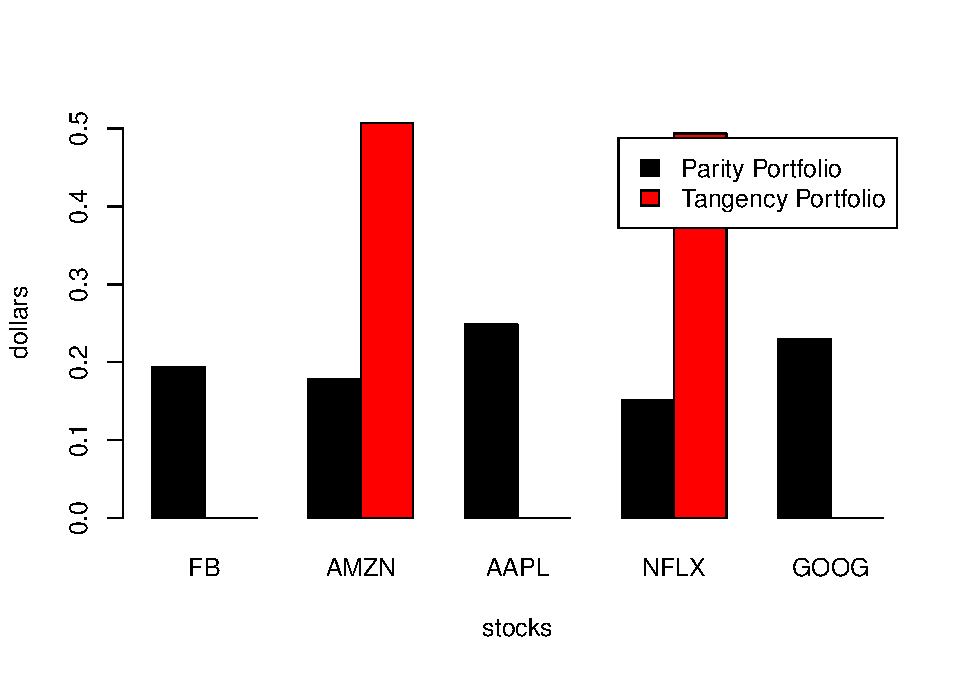
\includegraphics{open-quant-live-book_files/figure-latex/parityweights-1} 

}

\caption{Portfolio weights for parity and tangency FAANG portfolios considering returns from 2018.}\label{fig:parityweights}
\end{figure}

Fig. \ref{fig:parityrisks} compares the (covariance) risk budget of the
Parity and Tangency portfolios obtained. As expected, we observe that
the Parity portfolio has a risk budget equally distributed among the
portfolio assets. On the other hand, the Tangency portfolio concentrates
the risk between Amazon and Netflix with the latter corresponding to
over 56\% of the risk budget of the portfolio.

\begin{Shaded}
\begin{Highlighting}[]
\NormalTok{portfolio.risks <-}\StringTok{ }\KeywordTok{rbind}\NormalTok{(portfolio.parity}\OperatorTok{$}\NormalTok{risk_contribution}\OperatorTok{/}\KeywordTok{sum}\NormalTok{(portfolio.parity}\OperatorTok{$}\NormalTok{risk_contribution), }
  \KeywordTok{getCovRiskBudgets}\NormalTok{(portfolio.tangency))}
\KeywordTok{row.names}\NormalTok{(portfolio.risks) <-}\StringTok{ }\KeywordTok{c}\NormalTok{(}\StringTok{"Parity Portfolio"}\NormalTok{, }\StringTok{"Tangency Portfolio"}\NormalTok{)}
\KeywordTok{barplot}\NormalTok{(portfolio.risks, }\DataTypeTok{main =} \StringTok{""}\NormalTok{, }\DataTypeTok{xlab =} \StringTok{"stocks"}\NormalTok{, }\DataTypeTok{ylab =} \StringTok{"Covariance Risk Budget"}\NormalTok{, }
  \DataTypeTok{beside =} \OtherTok{TRUE}\NormalTok{, }\DataTypeTok{legend =} \OtherTok{TRUE}\NormalTok{, }\DataTypeTok{col =} \KeywordTok{c}\NormalTok{(}\StringTok{"black"}\NormalTok{, }\StringTok{"red"}\NormalTok{), }
  \DataTypeTok{args.legend =} \KeywordTok{list}\NormalTok{(}\DataTypeTok{bg =} \StringTok{"white"}\NormalTok{))}
\end{Highlighting}
\end{Shaded}

\begin{figure}[H]

{\centering 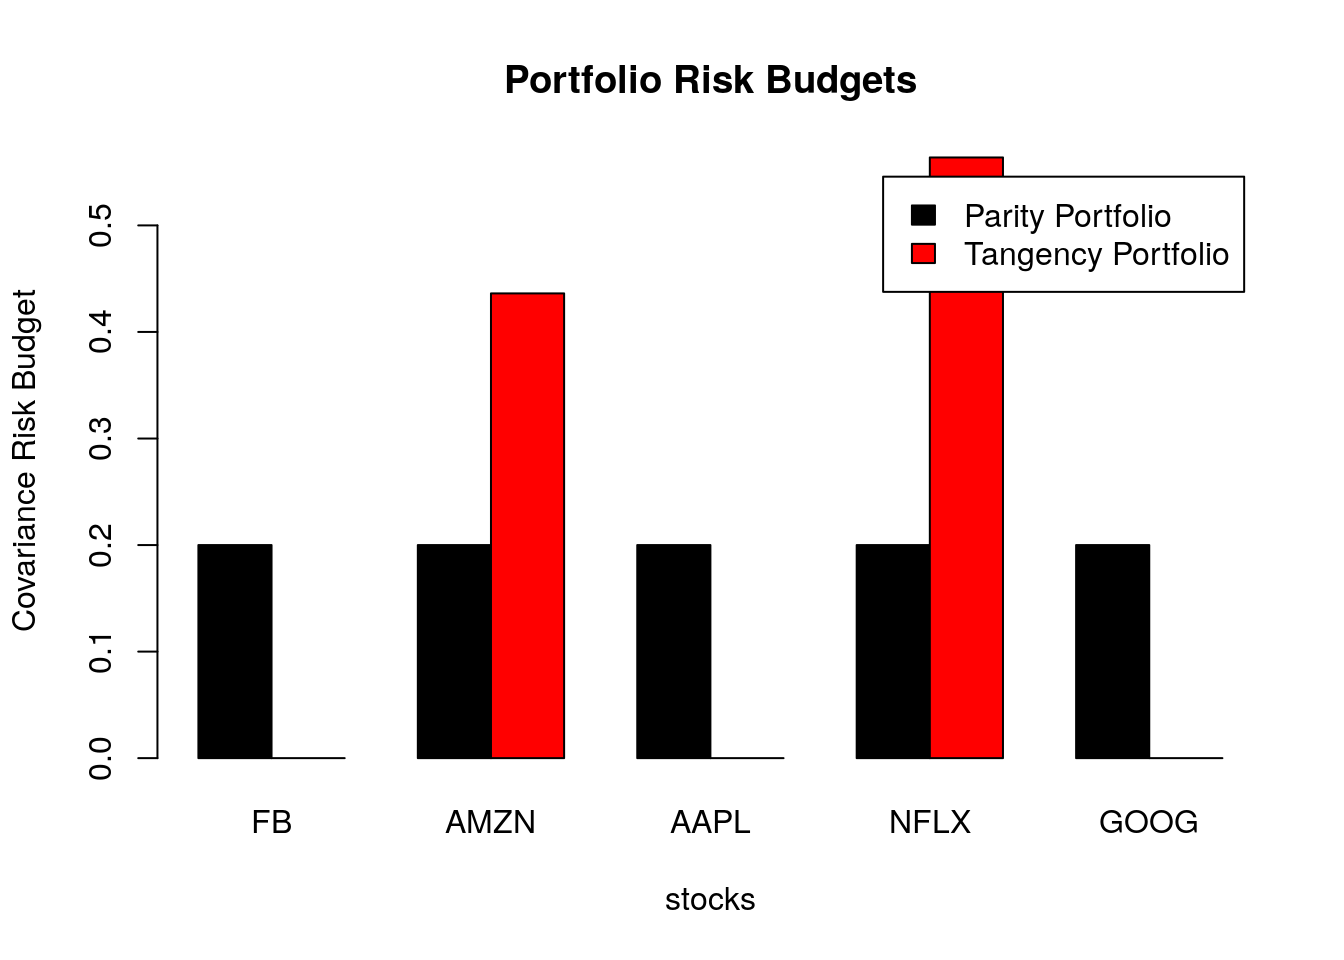
\includegraphics{open-quant-live-book_files/figure-latex/parityrisks-1} 

}

\caption{Portfolio covariance risk budget for parity and tangency FAANG portfolios considering returns from 2018.}\label{fig:parityrisks}
\end{figure}

\subsection{The Ray Dalio FAANG Index}\label{the-ray-dalio-faang-index}

What would be the performance of a ``Ray Dalio FAANG Index'' i.e.~a
portfolio composed of FAANG companies and rebalanced to match a
corresponding Risk Parity portfolio? Would it beat a corresponding
Tagency portfolio?

To answer these questions, we will consider a portfolio of FAANG
companies in the time period from 2014-01-01 and 2019-09-01 and build
two indices:

\begin{enumerate}
\def\labelenumi{\arabic{enumi}.}
\tightlist
\item
  Risk Parity Index: Rebalances portfolio weights quarterly setting the
  weights according to a risk parity portfolio;
\item
  Tangency Portfolio Index: Rebalances portfolio weights quarterly
  setting weights according to a Tangency portfolio.
\end{enumerate}

We first define our rebalance dates by constructing a rolling window of
12-month width and a 3-month step-size as follows:

\begin{Shaded}
\begin{Highlighting}[]
\KeywordTok{library}\NormalTok{(fPortfolio)}
\NormalTok{faang.returns.xts <-}\StringTok{ }\NormalTok{faang.returns[}\StringTok{"2014-01-01/2019-09-01"}\NormalTok{]}
\NormalTok{rWindows <-}\StringTok{ }\KeywordTok{rollingWindows}\NormalTok{(faang.returns.xts, }\DataTypeTok{period =} \StringTok{"12m"}\NormalTok{, }
  \DataTypeTok{by =} \StringTok{"3m"}\NormalTok{)}
\end{Highlighting}
\end{Shaded}

Our rebalance dates are the following:

\begin{Shaded}
\begin{Highlighting}[]
\KeywordTok{print}\NormalTok{(rWindows}\OperatorTok{$}\NormalTok{to)}
\end{Highlighting}
\end{Shaded}

\begin{verbatim}
## GMT
##  [1] [2014-12-31] [2015-03-31] [2015-06-30] [2015-09-30]
##  [5] [2015-12-31] [2016-03-31] [2016-06-30] [2016-09-30]
##  [9] [2016-12-31] [2017-03-31] [2017-06-30] [2017-09-30]
## [13] [2017-12-31] [2018-03-31] [2018-06-30] [2018-09-30]
## [17] [2018-12-31] [2019-03-31] [2019-06-30]
\end{verbatim}

Next, we calculate risk parity portfolio weights at each rebalance date
considering returns in a 12-month window as follows:

\begin{Shaded}
\begin{Highlighting}[]
\CommentTok{# Apply FUN to time-series R in the subset [from, to].}
\NormalTok{ApplyFilter <-}\StringTok{ }\ControlFlowTok{function}\NormalTok{(from, to, R, FUN) \{}
  \KeywordTok{return}\NormalTok{(}\KeywordTok{FUN}\NormalTok{(R[}\KeywordTok{paste0}\NormalTok{(from, }\StringTok{"/"}\NormalTok{, to)]))}
\NormalTok{\}}
\CommentTok{# For each pair (from, to) ApplyFilter to time-series R}
\CommentTok{# using FUN}
\NormalTok{ApplyRolling <-}\StringTok{ }\ControlFlowTok{function}\NormalTok{(from, to, R, FUN) \{}
  \KeywordTok{library}\NormalTok{(purrr)}
  \KeywordTok{return}\NormalTok{(}\KeywordTok{map2}\NormalTok{(from, to, ApplyFilter, }\DataTypeTok{R =}\NormalTok{ R, }\DataTypeTok{FUN =}\NormalTok{ FUN))}
\NormalTok{\}}
\CommentTok{# Returns weights of a risk parity portfolio from}
\CommentTok{# covariance matrix of matrix of returns r}
\NormalTok{CalculateRiskParity <-}\StringTok{ }\ControlFlowTok{function}\NormalTok{(r) \{}
  \KeywordTok{library}\NormalTok{(riskParityPortfolio)}
  \KeywordTok{return}\NormalTok{(}\KeywordTok{riskParityPortfolio}\NormalTok{(}\KeywordTok{cov}\NormalTok{(r))}\OperatorTok{$}\NormalTok{w)}
\NormalTok{\}}
\CommentTok{# Given a matrix of returns `r`, calculates risk parity}
\CommentTok{# weights for each date in `to` considering a time window}
\CommentTok{# from `from` and `to`}
\NormalTok{RollingRiskParity <-}\StringTok{ }\ControlFlowTok{function}\NormalTok{(from, to, r) \{}
  \KeywordTok{library}\NormalTok{(rlist)}
\NormalTok{  p <-}\StringTok{ }\KeywordTok{ApplyRolling}\NormalTok{(from, to, r, CalculateRiskParity)}
  \KeywordTok{names}\NormalTok{(p) <-}\StringTok{ }\NormalTok{to}
  \KeywordTok{return}\NormalTok{(}\KeywordTok{list.rbind}\NormalTok{(p))}
\NormalTok{\}}

\NormalTok{parity.weights <-}\StringTok{ }\KeywordTok{RollingRiskParity}\NormalTok{(rWindows}\OperatorTok{$}\NormalTok{from}\OperatorTok{@}\NormalTok{Data, rWindows}\OperatorTok{$}\NormalTok{to}\OperatorTok{@}\NormalTok{Data, }
\NormalTok{  faang.returns.xts)}
\end{Highlighting}
\end{Shaded}

We now calculate quarterly weights for FAANG tangency portfolios. We
leverage the \textbf{fPortfolio} package to calculate a rolling tangency
portfolio as follows:

\begin{Shaded}
\begin{Highlighting}[]
\KeywordTok{library}\NormalTok{(fPortfolio)}
\NormalTok{faang.returns.ts <-}\StringTok{ }\KeywordTok{as.timeSeries}\NormalTok{(faang.returns.xts)}
\NormalTok{Spec =}\StringTok{ }\KeywordTok{portfolioSpec}\NormalTok{()}

\NormalTok{rolling.portfolio.tangency <-}\StringTok{ }\KeywordTok{rollingTangencyPortfolio}\NormalTok{(faang.returns.ts, }
  \DataTypeTok{constraints =} \StringTok{"LongOnly"}\NormalTok{, }\DataTypeTok{from =}\NormalTok{ rWindows}\OperatorTok{$}\NormalTok{from, }\DataTypeTok{to =}\NormalTok{ rWindows}\OperatorTok{$}\NormalTok{to, }
  \DataTypeTok{spec =}\NormalTok{ Spec)}

\KeywordTok{names}\NormalTok{(rolling.portfolio.tangency) <-}\StringTok{ }\NormalTok{rWindows}\OperatorTok{$}\NormalTok{to}
\NormalTok{tan.weights <-}\StringTok{ }\KeywordTok{sapply}\NormalTok{(rolling.portfolio.tangency, getWeights)}
\KeywordTok{rownames}\NormalTok{(tan.weights) <-}\StringTok{ }\KeywordTok{colnames}\NormalTok{(faang.returns.ts)}
\NormalTok{tan.weights <-}\StringTok{ }\KeywordTok{t}\NormalTok{(tan.weights)}
\end{Highlighting}
\end{Shaded}

Figs. \ref{fig:rollingparityweights} and
\ref{fig:rollingtangencyweights} show the portfolio weights obtained for
parity risk and tangency portfolios, respectively. We observe that the
risk parity weights are quite stable over time with Netflix having a
slightly underweighting compared to the other portfolio constituents. On
the other hand, the tangency portfolio weights vary considerably
throughout the time period considered, which can impose challenges in
its maintenance as its turnover can be quite high. The tangency
portfolio overweights Apple and Amazon across many rebalance dates and
it underweights Google in all rebalance dates.

\begin{Shaded}
\begin{Highlighting}[]
\NormalTok{PerformanceAnalytics}\OperatorTok{::}\KeywordTok{chart.StackedBar}\NormalTok{(parity.weights, }\DataTypeTok{xlab =} \StringTok{"Rebalance Dates"}\NormalTok{, }
  \DataTypeTok{ylab =} \StringTok{"Weight"}\NormalTok{, }\DataTypeTok{main =} \StringTok{"FAANG Risk Parity"}\NormalTok{)}
\end{Highlighting}
\end{Shaded}

\begin{figure}[H]

{\centering 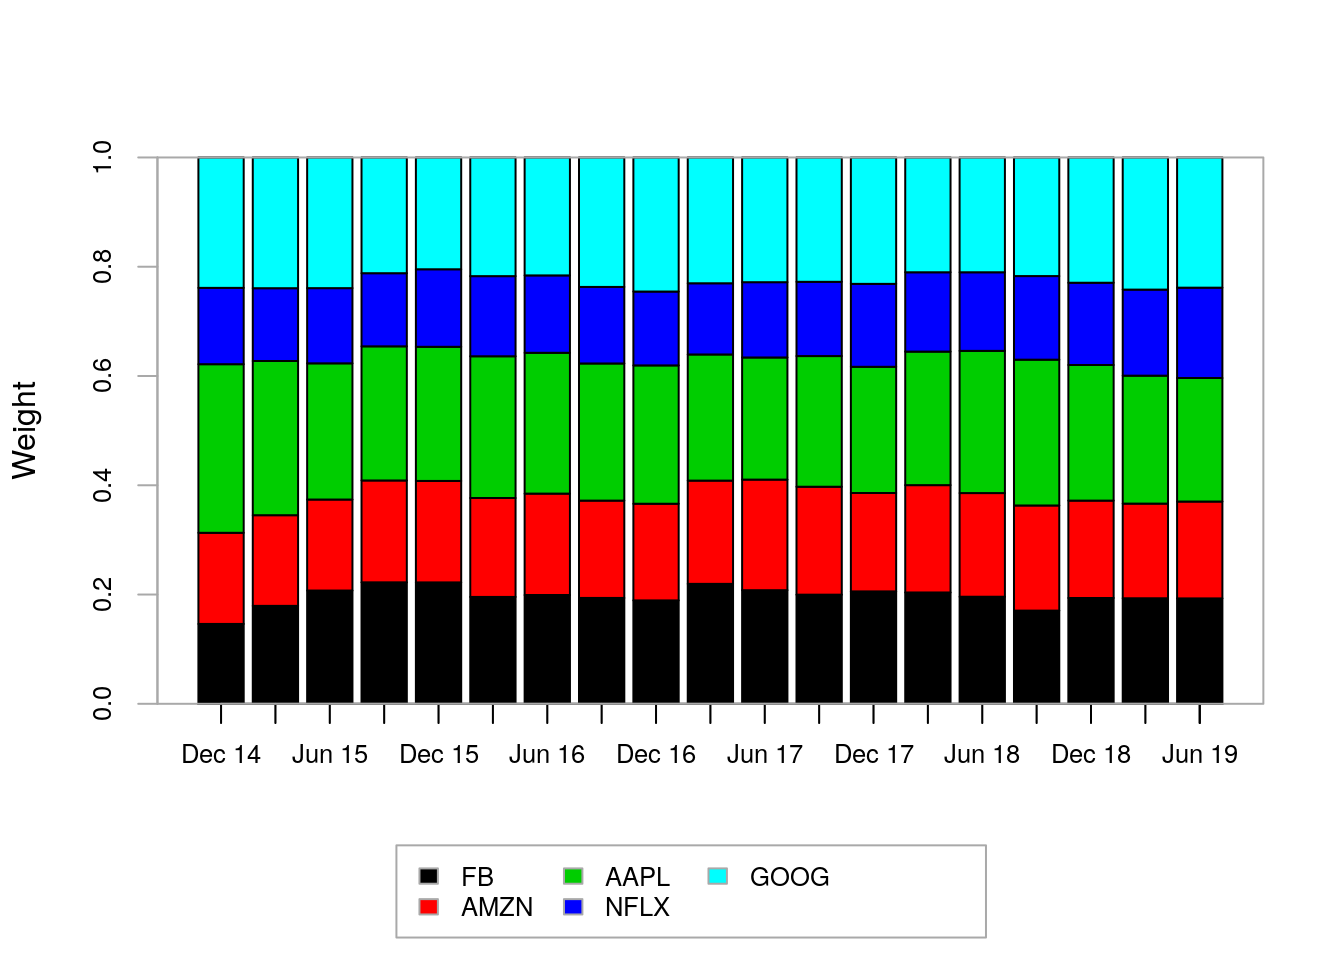
\includegraphics{open-quant-live-book_files/figure-latex/rollingparityweights-1} 

}

\caption{Portfolio weights for FAANG risk parity portfolios.}\label{fig:rollingparityweights}
\end{figure}

\begin{Shaded}
\begin{Highlighting}[]
\NormalTok{PerformanceAnalytics}\OperatorTok{::}\KeywordTok{chart.StackedBar}\NormalTok{(tan.weights, }\DataTypeTok{xlab =} \StringTok{"Rebalance Dates"}\NormalTok{, }
  \DataTypeTok{ylab =} \StringTok{"Weight"}\NormalTok{, }\DataTypeTok{main =} \StringTok{"FAANG Tangency Portfolio"}\NormalTok{)}
\end{Highlighting}
\end{Shaded}

\begin{figure}[H]

{\centering 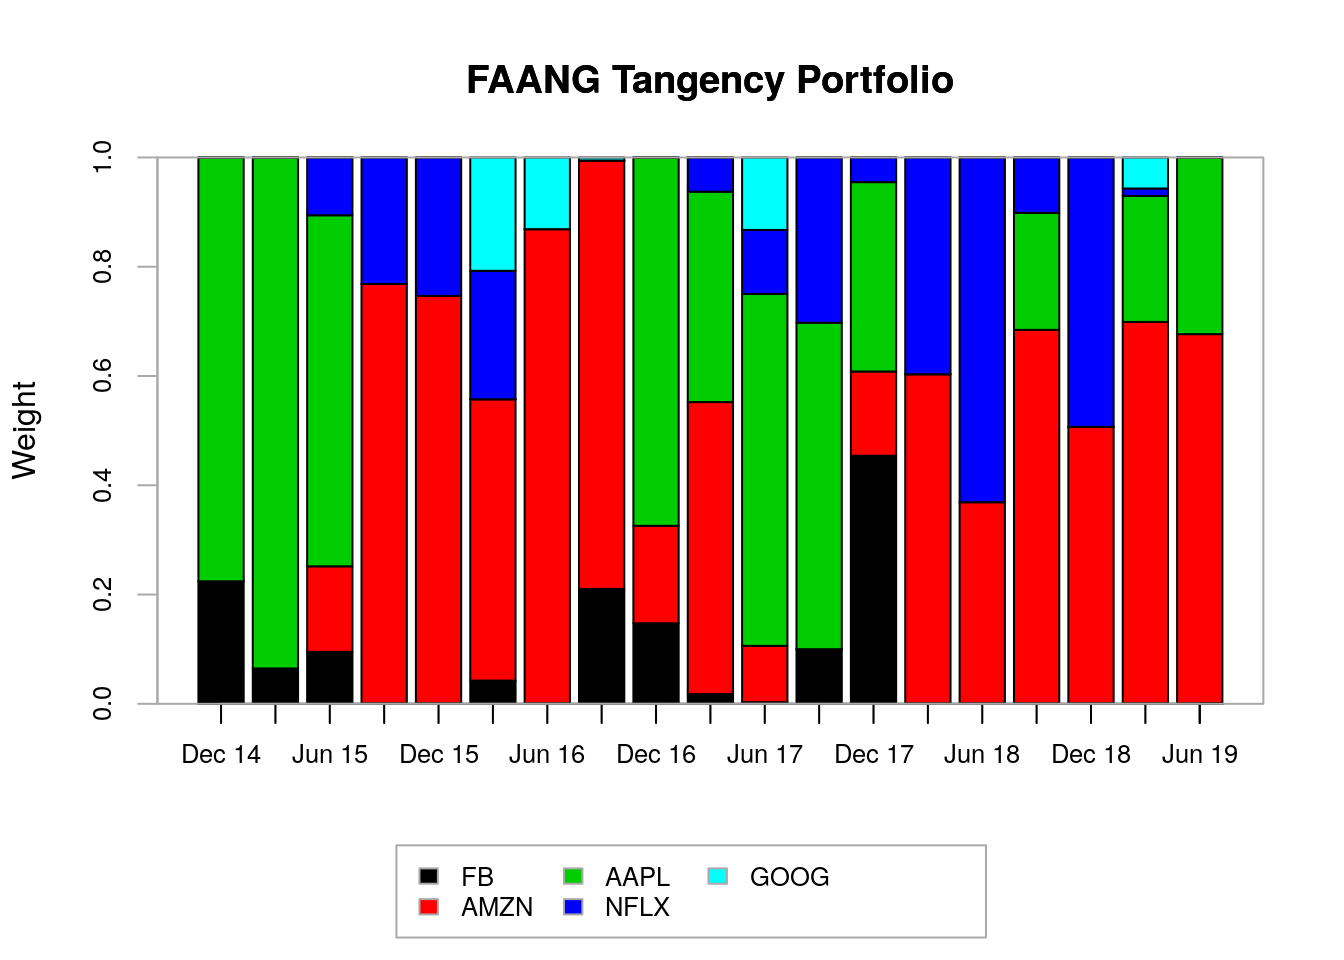
\includegraphics{open-quant-live-book_files/figure-latex/rollingtangencyweights-1} 

}

\caption{Portfolio weights for FAANG tangency portfolios.}\label{fig:rollingtangencyweights}
\end{figure}

We will use the time series of FAANG companies and the time series of
risk parity and tangency portfolio weights to calculate the returns of
the risk parity and tangency portfolio indexes as follows:

\begin{Shaded}
\begin{Highlighting}[]
\KeywordTok{library}\NormalTok{(PerformanceAnalytics)}
\NormalTok{tan.returns <-}\StringTok{ }\KeywordTok{Return.portfolio}\NormalTok{(faang.returns.xts, }\DataTypeTok{weights =}\NormalTok{ tan.weights, }
  \DataTypeTok{verbose =} \OtherTok{TRUE}\NormalTok{)}
\NormalTok{parity.returns <-}\StringTok{ }\KeywordTok{Return.portfolio}\NormalTok{(faang.returns.xts, }\DataTypeTok{weights =}\NormalTok{ parity.weights, }
  \DataTypeTok{verbose =} \OtherTok{TRUE}\NormalTok{)}
\NormalTok{p.returns <-}\StringTok{ }\KeywordTok{merge}\NormalTok{(tan.returns}\OperatorTok{$}\NormalTok{returns, parity.returns}\OperatorTok{$}\NormalTok{returns)}
\KeywordTok{names}\NormalTok{(p.returns) <-}\StringTok{ }\KeywordTok{c}\NormalTok{(}\StringTok{"FAANG Tangency Index"}\NormalTok{, }\StringTok{"FAANG Parity Index"}\NormalTok{)}
\end{Highlighting}
\end{Shaded}

Fig. \ref{fig:perfsummary} shows the performance summary for the risk
parity index versus the tangency portfolio index. Surprisingly, the
FAANG risk parity index outperforms the FAANG tangency portfolio index
by quite a bit with a cumulative return of 169.482\% versus 109.652\%
from the tangency portfolio index. The FAANG risk parity index also has
a relatively lower drawdown across most of the period analyzed.

\begin{Shaded}
\begin{Highlighting}[]
\NormalTok{### Performance Summary (return / drawdown)}
\NormalTok{PerformanceAnalytics}\OperatorTok{::}\KeywordTok{charts.PerformanceSummary}\NormalTok{(p.returns, }
  \DataTypeTok{colorset =}\NormalTok{ rich6equal, }\DataTypeTok{lwd =} \DecValTok{2}\NormalTok{, }\DataTypeTok{cex.legend =} \DecValTok{1}\NormalTok{, }\DataTypeTok{event.labels =} \OtherTok{TRUE}\NormalTok{, }
  \DataTypeTok{main =} \StringTok{""}\NormalTok{)}
\end{Highlighting}
\end{Shaded}

\begin{figure}[H]

{\centering 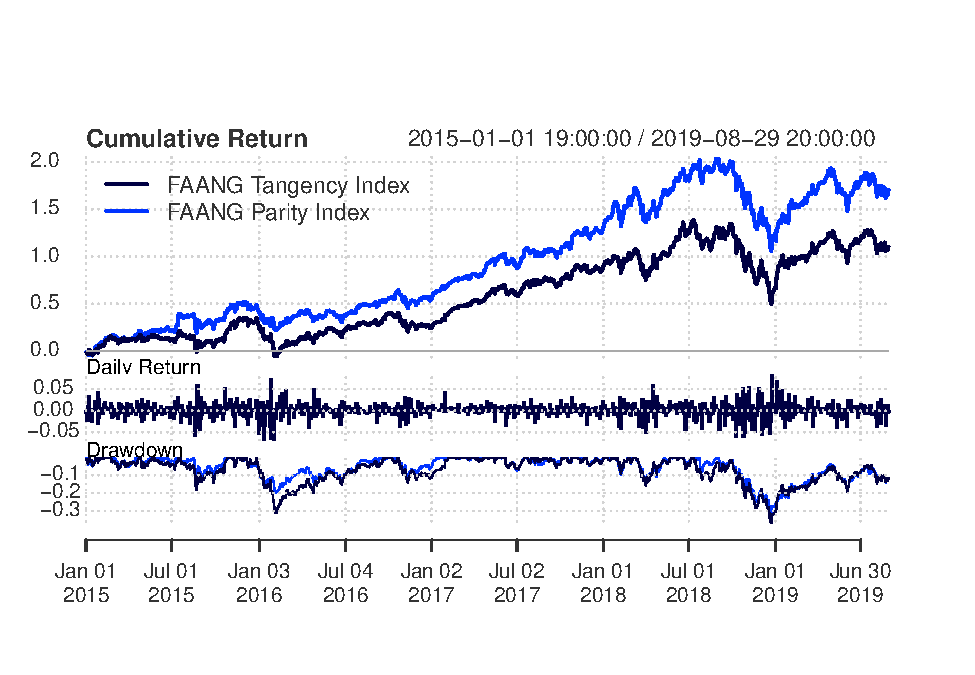
\includegraphics[width=1\linewidth]{open-quant-live-book_files/figure-latex/perfsummary-1} 

}

\caption{Performance summary for the risk parity index versus the tangency portfolio index}\label{fig:perfsummary}
\end{figure}

Tables \ref{tab:calretparity} and \ref{tab:calrettangency} show the
calendar returns for the risk parity and tangency portfolio indexes,
respectively. Interestingly, in years where the tangency portfolio index
had positive cumulative return, the risk parity index yielded less
returns than the tangency portfolio index. Conversely, in years where
the tangency portfolio index had negative cumulative return, the risk
parity index showed superior performance than the tangency portfolio
index. In that way, the risk parity index showed ``not as good'' but
also ``not as bad'' yearly returns compared to the tangency portfolios.

\textbackslash{}begin\{table\}{[}t{]}

\textbackslash{}caption\{\label{tab:calretparity}Calendar Returns (\%):
FAANG Parity Index\} \centering

\begin{tabular}{lrrrrr}
\toprule
  & 2015 & 2016 & 2017 & 2018 & 2019\\
\midrule
Jan & 2.1 & 0.6 & 2.1 & -0.6 & -1.2\\
Feb & -1.1 & 3.7 & 1.4 & -1.6 & 1.0\\
Mar & -0.6 & 1.3 & 0.0 & 2.3 & 1.6\\
Apr & 0.9 & 1.7 & 1.7 & 1.4 & 0.9\\
May & 0.4 & -0.6 & 0.1 & 1.8 & -2.2\\
\addlinespace
Jun & 0.6 & 1.3 & -0.4 & -0.4 & 1.3\\
Jul & -0.4 & 1.3 & 0.5 & 1.8 & -1.1\\
Aug & -4.2 & 0.2 & -0.1 & -0.2 & -0.4\\
Sep & 0.9 & 0.7 & 0.8 & 0.3 & NA\\
Oct & -0.7 & -1.0 & 0.2 & 1.7 & NA\\
\addlinespace
Nov & 1.8 & -1.2 & -0.9 & 0.3 & NA\\
Dec & -1.8 & -1.3 & -0.8 & 0.8 & NA\\
FAANG Parity Index & -2.1 & 6.9 & 4.6 & 7.8 & 0.0\\
\bottomrule
\end{tabular}

\textbackslash{}end\{table\} \textbackslash{}begin\{table\}{[}t{]}

\textbackslash{}caption\{\label{tab:calrettangency}Calendar Returns (\%):
FAANG Tangency Index\} \centering

\begin{tabular}{lrrrrr}
\toprule
  & 2015 & 2016 & 2017 & 2018 & 2019\\
\midrule
Jan & -1.7 & -1.0 & 4.5 & 0.6 & -2.6\\
Feb & -1.6 & 4.8 & 1.7 & -1.4 & 0.8\\
Mar & -0.3 & 1.5 & 0.0 & 2.4 & 2.4\\
Apr & 2.8 & 5.0 & 2.3 & 0.7 & 0.5\\
May & 0.3 & -0.5 & 0.2 & 1.4 & -2.1\\
\addlinespace
Jun & 1.0 & 2.1 & -0.4 & -0.5 & 1.6\\
Jul & -0.4 & 1.1 & 0.7 & 0.6 & -1.2\\
Aug & -4.6 & 0.2 & 0.0 & -0.3 & -0.4\\
Sep & 0.4 & 0.9 & 0.6 & 1.1 & NA\\
Oct & 0.5 & -0.7 & -0.4 & 3.6 & NA\\
\addlinespace
Nov & 2.0 & -1.3 & -0.5 & 0.5 & NA\\
Dec & -1.9 & -1.8 & -0.9 & 1.7 & NA\\
FAANG Tangency Index & -3.7 & 10.3 & 7.9 & 11.0 & -1.2\\
\bottomrule
\end{tabular}

\textbackslash{}end\{table\}

Fig. \ref{fig:rollingperfsummary} shows the performance summary in a
rolling 252-day window. Again, we observe that the risk parity index
presents a superior performance compared to the tangency portfolio
index. The risk parity index presents higher annualized return, lower
standard deviation and superior Sharpe ratio in most of the period
analyzed compared to the tangency portfolio index. As presented in Tab.
\ref{tab:annualret}, the risk parity index has a total of 23.71\%
annualized return, 22.55\% standard deviation and 1.051 Sharpe-ratio
versus 17.22\% annualized return, 26.42\% standard deviation and 0.652
Sharpe-ratio from the tangency portfolio index.

\begin{figure}[H]

{\centering 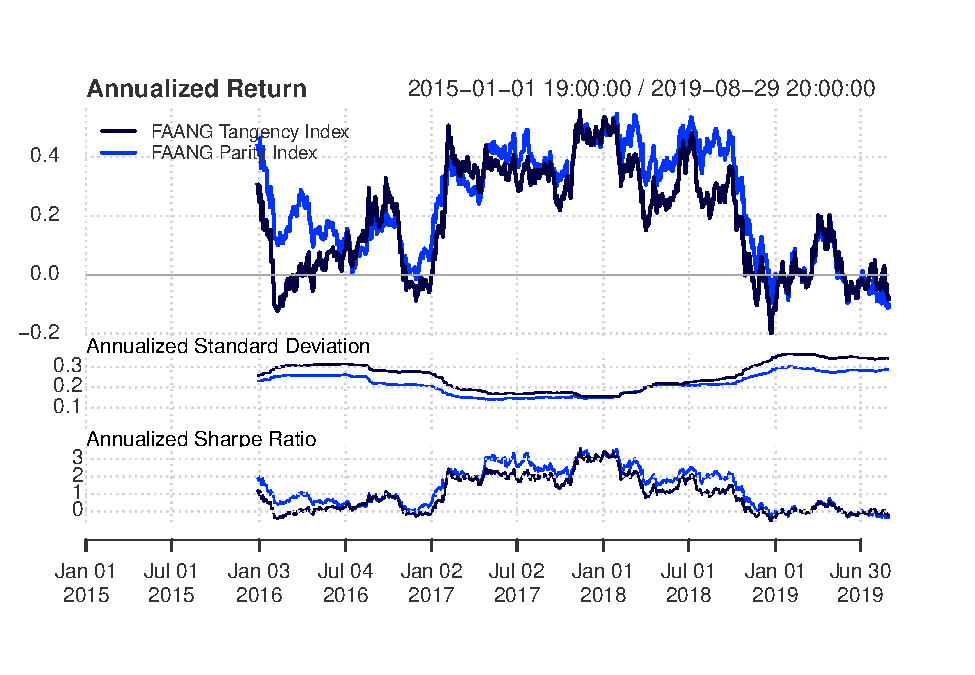
\includegraphics[width=1\linewidth]{open-quant-live-book_files/figure-latex/rollingperfsummary-1} 

}

\caption{Performance summary in a rolling 252-day window for the risk parity index versus the tangency portfolio index}\label{fig:rollingperfsummary}
\end{figure}

\begin{table}[t]

\caption{\label{tab:annualret}Annualized Returns}
\centering
\begin{tabular}{lrr}
\toprule
  & FAANG Tangency Index & FAANG Parity Index\\
\midrule
Annualized Return & 0.172 & 0.237\\
Annualized Std Dev & 0.264 & 0.226\\
Annualized Sharpe (Rf=0\%) & 0.652 & 1.051\\
\bottomrule
\end{tabular}
\end{table}

\section{Discussion and Conclusion}\label{discussion-and-conclusion}

\emph{What mix of assets has the best chance of delivering good returns
over time through all economic environments?}

That was the question posed by Bridgewater Associates before creating
the All Weather funds with concepts today popularized in the so-called
risk parity strategies.

The traditional approach to asset allocation often tolerates higher
concentration of risk with the objective to generate higher longer-term
returns. Bridgewater argues that this approach has a serious flaw:

\begin{quote}
If the source of short-term risk is a heavy concentration in a single
type of asset, this approach brings with it a significant risk of poor
long-term returns that threatens the ability to meet future obligations.
This is because every asset is susceptible to poor performance that can
last for a decade or more, caused by a sustained shift in the economic
environment - Bridgewater.
\end{quote}

In this Chapter, we introduced the concept of risk parity portfolios and
compare it against a mean-variance model. We provided a simple practical
example by constructing a FAANG risk parity index and comparing its
performance against a FAANG tangency index, which selects the portfolio
from the mean-variance efficient frontier with optimal Sharpe-ratio.

The risk parity index presented higher annualized return, lower standard
deviation and superior Sharpe ratio in most of the period analyzed
compared to the tangency portfolio index. Of course, results should be
taken with caution.

In practice, both the risk parity and mean-variance approaches are
employed in larger portfolios potentially across multiple asset classes.
Those methodologies strive when there are assets that are uncorrelated
in the portfolio which can increase the potential for diversification.
Further, modern portfolio optimization strategies can be much more
complex with a variety of objective functions and constraints. Our
objective in this article was to give you a head start. Feel free to
check out the source code in our github project and implement your own
strategies!

\part{Machine Learning}\label{part-machine-learning}

\part{Econophysics}\label{part-econophysics}

\chapter{Entropy}\label{entropy}

\section{Definition}\label{definition}

Let \(X\) be a random variable and \(P_X(x)\) be its probability density
function (pdf). The entropy \(H(X)\) can be interpreted sa measure of
the uncertainty of \(X\) and is defined in the discrete case as follows:

\begin{equation}
H(X) = -\sum_{x \in X}{P_X(x)\log{P_X(x)}}.
\label{eq:H}
\end{equation}

If the \(\log\) is taken to base two, then the unit of \(H\) is the
\textit{bit} (binary digit). We employ the natural logarithm which
implies the unit in \textit{nat} (natural unit of information).

\section{Nonlinear Coupling}\label{nonlinear-coupling}

\subsection{Simulated Systems}\label{simulated-systems}

\subsection{Equity-Commodities
Relationship}\label{equity-commodities-relationship}

\section{Efficiency and Bubbles: A Case Study in the Crypto and Equity
Markets}\label{efficiency-and-bubbles-a-case-study-in-the-crypto-and-equity-markets}

\chapter{How to Measure Statistical Causality: A Transfer Entropy
Approach with Financial
Applications}\label{how-to-measure-statistical-causality-a-transfer-entropy-approach-with-financial-applications}

We've all heard the say ``correlation does not imply causation'', but
how can we quantify causation? This is an extremely difficult and often
misleading task, particularly when trying to infer causality from
observational data and we cannot perform controlled trials or A/B
testing.

Take for example the 2-dimensional system from Fig. \ref{fig:rand}.

\begin{figure}[H]

{\centering 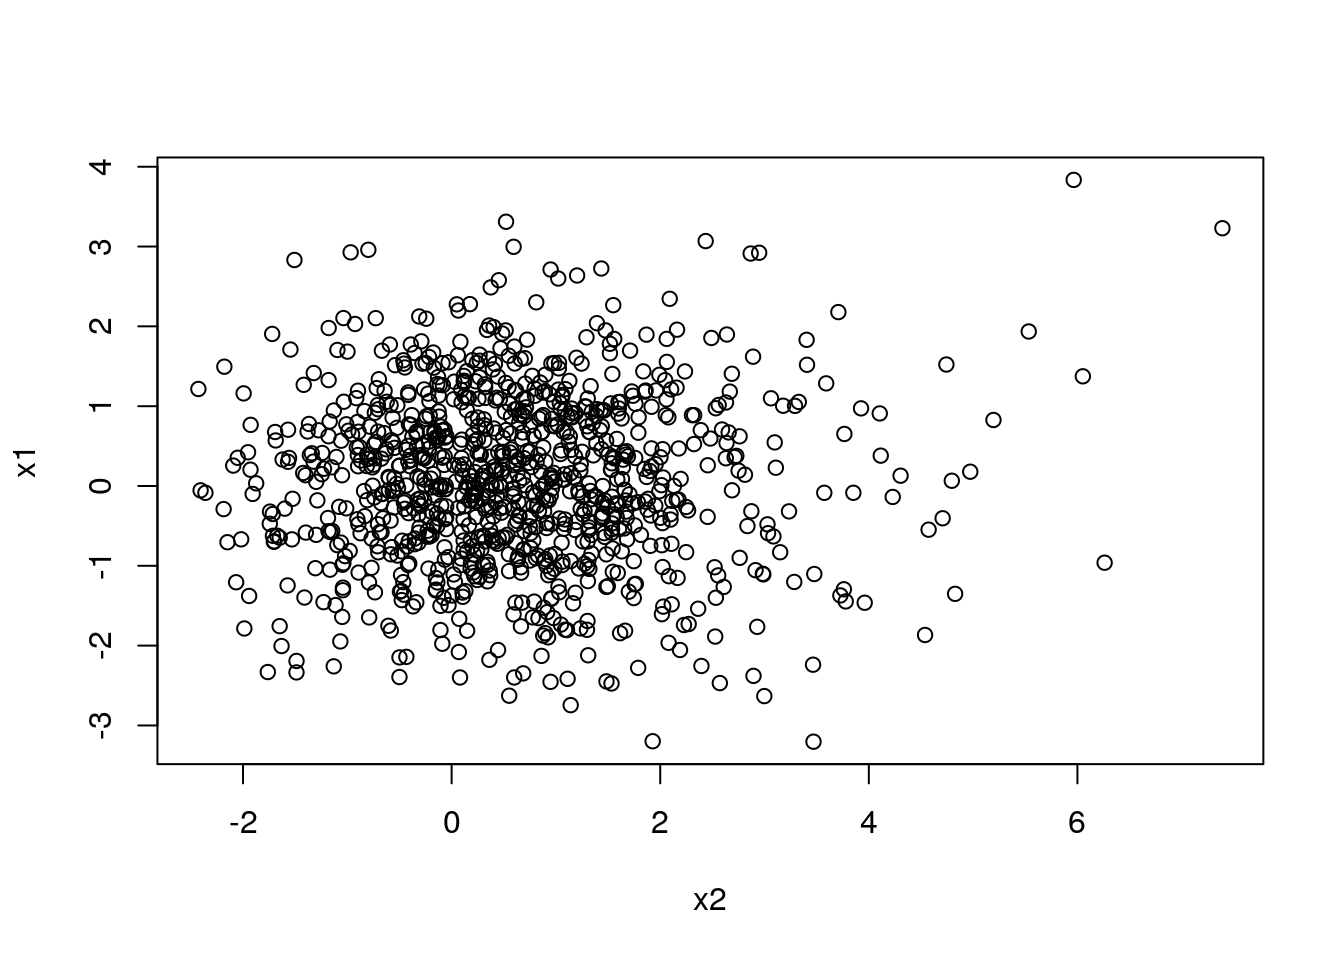
\includegraphics[width=0.5\linewidth]{open-quant-live-book_files/figure-latex/rand-1} 

}

\caption{Life is Random (or Nonlinear?)}\label{fig:rand}
\end{figure}

At a first glance, one could say that there is no clear relationship or
causality between the random variables \(x_1\) and \(x_2\). However,
this apparent random system presents a causal relationship defined by
the following simple equations:

\begin{align*}
x_1(n) &= 0.441x_1(n-1) + \epsilon_1 \\
x_2(n) &= 0.51x_1^2(n-1) + \epsilon_2, \\ 
&\epsilon_1, \epsilon_2 \sim \mathcal{N}(0,1).
\end{align*}

A simple nonlinearity introduced in the relationship between \(x_2\) and
\(x_1\) was enough to introduce complexity into the system and
potentially mislead a naive (non-quant) human.

Fortunately, we can take advantage of statistics and information theory
to uncover complex causal relationships from observational data
(remember, this is still a very challenging task).

The objectives of this Chapter are the following:

\begin{itemize}
\tightlist
\item
  Introduce a prediction-based definition of causality and its
  implementation using a vector auto-regression formulation.
\item
  Introduce a probabilistic-definition of causality and its
  implementation using an information-theoretical framework.
\item
  Simulate linear and nonlinear systems and uncover causal links with
  the proposed methods.
\item
  Quantify information flow among global equity indexes further
  uncovering which indexes are driving the global financial markets.
\item
  Discuss further applications including the impact of social media
  sentiment in financial and crypto markets.
\end{itemize}

\section{A First Definition of Causality}\label{LinearG}

We quantify causality by using the notion of the causal relation
introduced by Granger \citep{Wiener56, granger:econ}, where a signal
\(X\) is said to Granger-cause \(Y\) if the future realizations of \(Y\)
can be better explained using the past information from \(X\) and \(Y\)
rather than \(Y\) alone.

\begin{figure}[H]

{\centering 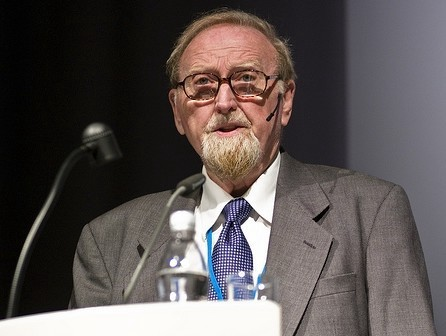
\includegraphics[width=0.5\linewidth]{./chapters/TransferEntropy/G} 

}

\caption{Economist Clive Granger, who won the 2003 Nobel Prize in Economics.}\label{fig:G}
\end{figure}

The most common definitions of Granger-causality (\emph{G-causality})
rely on the prediction of a future value of the variable \(Y\) by using
the past values of \(X\) and \(Y\) itself. In that form, \(X\) is said
to \emph{G-cause} \(Y\) if the use of \(X\) improves the prediction of
\(Y\).

Let \(X_t\) be a random variable associated at time \(t\) while \(X^t\)
represents the collection of random variables up to time \(t\). We
consider \({X_t}, {Y_t}\) and \({Z_t}\) to be three stochastic
processes. Let \(\hat Y_{t+1}\) be a predictor for the value of the
variable \(Y\) at time \(t+1\).

We compare the expected value of a loss function \(g(e)\) with the error
\(e=\hat{Y}_{t+1} - Y_{t+1}\) of two models:

\begin{enumerate}
\def\labelenumi{\arabic{enumi}.}
\tightlist
\item
  The expected value of the prediction error given only \(Y^t\)

  \begin{equation}
   \mathcal{R}(Y^{t+1} \, | \, Y^t,Z^t) = \mathbb{E}[g(Y_{t+1} - f_1(X^{t},Z^t))]
  \end{equation}
\item
  The expected value of the prediction error given \(Y^t\) and \(X^t\)

  \begin{equation}
   \mathcal{R}(Y^{t+1} \, | \, X^{t},Y^t,Z^t) = \mathbb{E}[g(Y_{t+1} - f_2(X^{t},Y^t,Z^t))].
  \end{equation}
\end{enumerate}

In both models, the functions \(f_1(.)\) and \(f_2(.)\) are chosen to
minimize the expected value of the loss function. In most cases, these
functions are retrieved with linear and, possibly, with nonlinear
regressions, neural networks etc. Typical forms for \(g(.)\) are the
\(l1\)- or \(l2\)-norms.

We can now provide our first definition of statistical causality under
the Granger causal notion as follows:

\BeginKnitrBlock{definition}
\protect\hypertarget{def:G1}{}{\label{def:G1} }\(X\) does not Granger-cause
\(Y\) relative to side information \(Z\) if and only if
\(\mathcal{R}(Y_{t+1} \; | \; X^t, Y^t, Z^t) = \mathcal{R}(Y_{t+1} \; | \; Y^t, Z^t)\).
\EndKnitrBlock{definition}

Standard Granger-causality tests assume a functional form in the
relationship among the causes and effects and are implemented by fitting
autoregressive models \citep{Wiener56, granger:econ}.

Consider the linear vector-autoregressive (VAR) equations:

\begin{align}
Y(t) &= {\alpha} + \sum^k_{\Delta t=1}{{\beta}_{\Delta t} Y(t-\Delta t)} + \epsilon_t, \label{eq:AR11}\\
Y(t) &= \widehat{\alpha} + \sum^k_{\Delta t=1}{{\widehat{\beta}}_{\Delta t} Y(t-\Delta t)} +  \sum^k_{\Delta t=1}{{\widehat{\gamma}}_{\Delta t}X(t-\Delta t)}+ \widehat{\epsilon}_t, \label{eq:AR22}
\end{align}

where \(k\) is the number of lags considered. Alternatively, you can
choose your DL/SVM/RF/GLM method of choice to fit the model.

From Def. \ref{def:G1}, \(X\) does not G-cause \(Y\) if and only if the
prediction errors of \(X\) in the restricted Eq. \eqref{eq:AR11} and
unrestricted regression models Eq. \eqref{eq:AR22} are equal (i.e., they
are statistically indistinguishable). A one-way ANOVA test can be
utilized to test if the residuals from Eqs. \eqref{eq:AR11} and
\eqref{eq:AR22} differ from each other significantly. When more than one
lag \(k\) is tested, a correction for multiple hypotheses testing should
be applied, e.g.~False Discovery Rate (FDR) or Bonferroni correction.

\section{A Probabilistic-Based
Definition}\label{a-probabilistic-based-definition}

A more general definition than Def. \ref{def:G1} that does not depend on
assuming prediction functions can be formulated by considering
conditional probabilities. A probabilistic definition of G-causality
assumes that \(Y_{t+1}\) and \(X^{t}\) are independent given the past
information \((X^{t}, Y^{t})\) if and only if
\(p(Y_{t+1} \, | \, X^{t}, Y^{t}, Z^{t}) = p(Y_{t+1} \, | \, Y^{t}, Z^{t})\),
where \(p(. \, | \, .)\) represents the conditional probability
distribution. In other words, omitting past information from \(X\) does
not change the probability distribution of \(Y\). This leads to our
second definition of statistical causality as follows:

\BeginKnitrBlock{definition}
\protect\hypertarget{def:G2}{}{\label{def:G2} }\(X\) does not Granger-cause
\(Y\) relative to side information \(Z\) if and only if
\(Y_{t+1} \independent X^{t} \; | \; Y^{t}, Z^{t}\).
\EndKnitrBlock{definition}

Def. \ref{def:G2} does not assume any functional form in the coupling
between \(X\) and \(Y\). Nevertheless, it requires a method to assess
their conditional dependency. In the next section, we will leverage an
Information-Theoretical framework for that purpose.

\section{Transfer Entropy and Statistical Causality}\label{nonlinearG}

Given a coupled system \((X,Y)\), where \(P_Y(y)\) is the pdf of the
random variable \(Y\) and \(P_{X,Y}\) is the joint pdf between \(X\) and
\(Y\), the joint entropy between \(X\) and \(Y\) is given by the
following:

\begin{equation}
H(X,Y) = -\sum_{x \in X}{\sum_{y \in Y}{P_{X,Y}(x,y)\log{P_{X,Y}(x,y)}}}.
\label{eq:HXY}
\end{equation}

The conditional entropy is defined by the following:

\begin{equation}
H\left(Y\middle\vert X\right) = H(X,Y) - H(X).
\end{equation}

We can interpret \(H\left(Y\middle\vert X\right)\) as the uncertainty of
\(Y\) given a realization of \(X\).

\begin{figure}[H]

{\centering 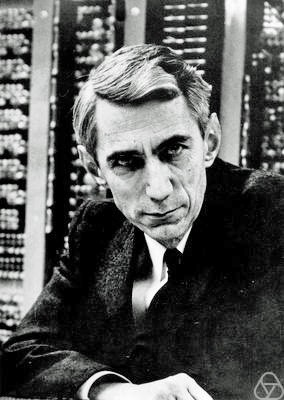
\includegraphics[width=0.5\linewidth]{./chapters/TransferEntropy/S} 

}

\caption{Shannon, Claude. The concept of information entropy was introduced by Claude Shannon in his 1948 paper: A Mathematical Theory of Communication.}\label{fig:S}
\end{figure}

To compute G-Causality, we use the concept of Transfer Entropy. Since
its introduction \citep{PhysRevLett.85.461}, Transfer Entropy has been
recognized as an important tool in the analysis of causal relationships
in nonlinear systems \citep{citeulike:1447442}. It detects directional
and dynamical information \citep{10.1371/journal.pone.0109462} while not
assuming any particular functional form to describe interactions among
systems.

The Transfer Entropy can be defined as the difference between the
conditional entropies:

\begin{equation}
 TE\left(X \rightarrow Y\right \vert Z) =  H\left(Y^F\middle\vert Y^P,Z^P\right) - H\left(Y^F\middle\vert X^P, Y^P,Z^P\right),
\label{eq:TE}
\end{equation}

which can be rewritten as a sum of Shannon entropies:

\begin{align}
TE\left(X \rightarrow Y\right) = H\left(Y^P, X^P\right) - H\left(Y^F, Y^P, X^P\right) + H\left(Y^F, Y^P\right) - H\left(Y^P\right),
\end{align}

where \(Y^F\) is a forward time-shifted version of \(Y\) at lag
\(\Delta t\) relatively to the past time-series \(X^P\), \(Y^P\) and
\(Z^P\). Within this framework we say that \(X\) does not G-cause \(Y\)
relative to side information \(Z\) if and only if
\(H\left(Y^F\middle\vert Y^P,Z^P \right) = H\left(Y^F\middle\vert X^P, Y^P,Z^P\right)\),
i.e., when \(TE\left(X \rightarrow Y,Z^P\right) = 0\).

\section{Net Information Flow}\label{net-information-flow}

Transfer-entropy is an asymmetric measure, i.e.,
\(T_{X \rightarrow Y} \neq T_{Y \rightarrow X}\), and it thus allows the
quantification of the directional coupling between systems. The Net
Information Flow is defined as

\begin{equation}
\widehat{TE}_{X \rightarrow Y} = TE_{X \rightarrow Y} - TE_{Y \rightarrow X}\;.
\end{equation}

One can interpret this quantity as a measure of the dominant direction
of the information flow. In other words, a positive result indicates a
dominant information flow from \(X\) to \(Y\) compared to the other
direction or, similarly, it indicates which system provides more
predictive information about the other system
\citep{Michalowicz:2013:HDE:2601840}.

\section{The Link Between Granger-causality and Transfer
Entropy}\label{the-link-between-granger-causality-and-transfer-entropy}

It has been shown \citep{PhysRevLett.103.238701} that linear G-causality
and Transfer Entropy are equivalent if all processes are jointly
Gaussian. In particular, by assuming the standard measure (\(l2\)-norm
loss function) of linear G-causality for the bivariate case as follows
(see Section \ref{LinearG} for more details on linear-Granger
causality):

\begin{equation}
GC_{X \rightarrow Y} = \log\left( \frac{var(\epsilon_t)}{var( \widehat{\epsilon}_t)} \right),
\label{eq:GCGC}
\end{equation}

the following can be proved \citep{PhysRevLett.103.238701}:

\begin{align}
TE_{X \rightarrow Y} = GC_{X \rightarrow Y}/2.
\label{eq:GCGC2}
\end{align}

This result provides a direct mapping between the Transfer Entropy and
the linear G-causality implemented in the standard VAR framework. Hence,
it is possible to estimate the TE both in its general form and with its
equivalent form for linear G-causality.

\section{Information Flow on Simulated
Systems}\label{information-flow-on-simulated-systems}

In this section, we construct simulated systems to couple random
variables in a causal manner. We then quantify information flow using
the methods studied in this Chapter.

We first assume a linear system, where random variables have linear
relationships defined as follow:

\begin{align}
x_1(n) &= 0.95\sqrt{2}x_1(n-1) - 0.9025x_1(n-1) + w_1\\ \nonumber
x_2(n) &= 0.5x_1(n-1) + w_2\\ \nonumber
x_3(n) &= -0.4x_1(n-1) + w_3\\ \nonumber
x_4(n) &= -0.5x_1(n-1) + 0.25\sqrt{2}x_4(n-1) + 0.25\sqrt{2}x_5(n-1) + w_4\\ \nonumber
x_5(n) &= -0.25\sqrt{2}x_4(n-1) + 0.25\sqrt{2}x_5(n-1) + w_5, \nonumber
\end{align}

where \(w_1, w_2, w_3, w_4, w_5 \sim N(0, 1)\). To simulate this system
we assume \(x_i(0) = 0, i \in (1, 2, \ldots, 5)\) as initial condition
and then iteratively generate \(x_i\) for \(n \in (1, 2, \ldots, N)\)
with a total of \(N = 10,000\) iterations by randomly sampling
\(w_i, i \in (1, 2, \ldots, 5)\) from a normal distribution with zero
mean and unit variance.

We simulate this linear system with the following code:

\begin{Shaded}
\begin{Highlighting}[]
\KeywordTok{set.seed}\NormalTok{(}\DecValTok{123}\NormalTok{)}
\NormalTok{n <-}\StringTok{ }\DecValTok{10000}
\NormalTok{x1 <-}\StringTok{ }\NormalTok{x2 <-}\StringTok{ }\NormalTok{x3 <-}\StringTok{ }\NormalTok{x4 <-}\StringTok{ }\NormalTok{x5 <-}\StringTok{ }\KeywordTok{rep}\NormalTok{(}\DecValTok{0}\NormalTok{, n }\OperatorTok{+}\StringTok{ }\DecValTok{1}\NormalTok{)}

\ControlFlowTok{for}\NormalTok{ (i }\ControlFlowTok{in} \DecValTok{2}\OperatorTok{:}\NormalTok{(n }\OperatorTok{+}\StringTok{ }\DecValTok{1}\NormalTok{)) \{}
\NormalTok{  x1[i] <-}\StringTok{ }\FloatTok{0.95} \OperatorTok{*}\StringTok{ }\KeywordTok{sqrt}\NormalTok{(}\DecValTok{2}\NormalTok{) }\OperatorTok{*}\StringTok{ }\NormalTok{x1[i }\OperatorTok{-}\StringTok{ }\DecValTok{1}\NormalTok{] }\OperatorTok{-}\StringTok{ }\FloatTok{0.9025} \OperatorTok{*}\StringTok{ }\NormalTok{x1[i }\OperatorTok{-}\StringTok{ }
\StringTok{    }\DecValTok{1}\NormalTok{] }\OperatorTok{+}\StringTok{ }\KeywordTok{rnorm}\NormalTok{(}\DecValTok{1}\NormalTok{, }\DataTypeTok{mean =} \DecValTok{0}\NormalTok{, }\DataTypeTok{sd =} \DecValTok{1}\NormalTok{)}
\NormalTok{  x2[i] <-}\StringTok{ }\FloatTok{0.5} \OperatorTok{*}\StringTok{ }\NormalTok{x1[i }\OperatorTok{-}\StringTok{ }\DecValTok{1}\NormalTok{] }\OperatorTok{+}\StringTok{ }\KeywordTok{rnorm}\NormalTok{(}\DecValTok{1}\NormalTok{, }\DataTypeTok{mean =} \DecValTok{0}\NormalTok{, }\DataTypeTok{sd =} \DecValTok{1}\NormalTok{)}
\NormalTok{  x3[i] <-}\StringTok{ }\OperatorTok{-}\FloatTok{0.4} \OperatorTok{*}\StringTok{ }\NormalTok{x1[i }\OperatorTok{-}\StringTok{ }\DecValTok{1}\NormalTok{] }\OperatorTok{+}\StringTok{ }\KeywordTok{rnorm}\NormalTok{(}\DecValTok{1}\NormalTok{, }\DataTypeTok{mean =} \DecValTok{0}\NormalTok{, }\DataTypeTok{sd =} \DecValTok{1}\NormalTok{)}
\NormalTok{  x4[i] <-}\StringTok{ }\OperatorTok{-}\FloatTok{0.5} \OperatorTok{*}\StringTok{ }\NormalTok{x1[i }\OperatorTok{-}\StringTok{ }\DecValTok{1}\NormalTok{] }\OperatorTok{+}\StringTok{ }\FloatTok{0.25} \OperatorTok{*}\StringTok{ }\KeywordTok{sqrt}\NormalTok{(}\DecValTok{2}\NormalTok{) }\OperatorTok{*}\StringTok{ }\NormalTok{x4[i }\OperatorTok{-}\StringTok{ }\DecValTok{1}\NormalTok{] }\OperatorTok{+}\StringTok{ }
\StringTok{    }\FloatTok{0.25} \OperatorTok{*}\StringTok{ }\KeywordTok{sqrt}\NormalTok{(}\DecValTok{2}\NormalTok{) }\OperatorTok{*}\StringTok{ }\NormalTok{x5[i }\OperatorTok{-}\StringTok{ }\DecValTok{1}\NormalTok{] }\OperatorTok{+}\StringTok{ }\KeywordTok{rnorm}\NormalTok{(}\DecValTok{1}\NormalTok{, }\DataTypeTok{mean =} \DecValTok{0}\NormalTok{, }\DataTypeTok{sd =} \DecValTok{1}\NormalTok{)}
\NormalTok{  x5[i] <-}\StringTok{ }\OperatorTok{-}\FloatTok{0.25} \OperatorTok{*}\StringTok{ }\KeywordTok{sqrt}\NormalTok{(}\DecValTok{2}\NormalTok{) }\OperatorTok{*}\StringTok{ }\NormalTok{x4[i }\OperatorTok{-}\StringTok{ }\DecValTok{1}\NormalTok{] }\OperatorTok{+}\StringTok{ }\FloatTok{0.25} \OperatorTok{*}\StringTok{ }\KeywordTok{sqrt}\NormalTok{(}\DecValTok{2}\NormalTok{) }\OperatorTok{*}\StringTok{ }
\StringTok{    }\NormalTok{x5[i }\OperatorTok{-}\StringTok{ }\DecValTok{1}\NormalTok{] }\OperatorTok{+}\StringTok{ }\KeywordTok{rnorm}\NormalTok{(}\DecValTok{1}\NormalTok{, }\DataTypeTok{mean =} \DecValTok{0}\NormalTok{, }\DataTypeTok{sd =} \DecValTok{1}\NormalTok{)}
\NormalTok{\}}

\NormalTok{x1 <-}\StringTok{ }\NormalTok{x1[}\OperatorTok{-}\DecValTok{1}\NormalTok{]}
\NormalTok{x2 <-}\StringTok{ }\NormalTok{x2[}\OperatorTok{-}\DecValTok{1}\NormalTok{]}
\NormalTok{x3 <-}\StringTok{ }\NormalTok{x3[}\OperatorTok{-}\DecValTok{1}\NormalTok{]}
\NormalTok{x4 <-}\StringTok{ }\NormalTok{x4[}\OperatorTok{-}\DecValTok{1}\NormalTok{]}
\NormalTok{x5 <-}\StringTok{ }\NormalTok{x5[}\OperatorTok{-}\DecValTok{1}\NormalTok{]}
\NormalTok{linear.system <-}\StringTok{ }\KeywordTok{data.frame}\NormalTok{(x1, x2, x3, x4, x5)}
\end{Highlighting}
\end{Shaded}

The Fig. \ref{fig:causality-graph1} represents the dependencies of the
simulated linear system.

\begin{figure}[H]

{\centering 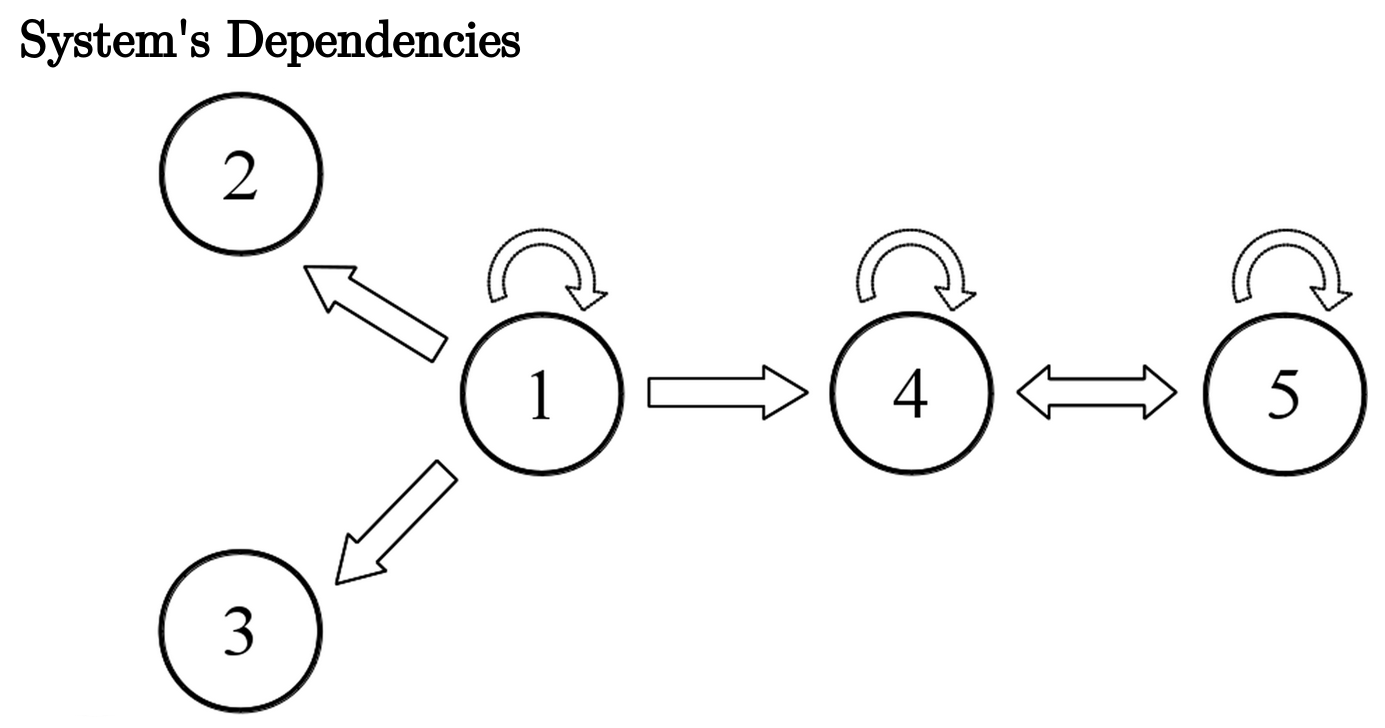
\includegraphics[width=1\linewidth]{./chapters/TransferEntropy/S4Fig1} 

}

\caption{Interactions between the variables of the simulated linear system.}\label{fig:causality-graph1}
\end{figure}

We first define a function that calculates a bi-variate measure for
G-causality as defined in Eq. \eqref{eq:GCGC} as follows:

\begin{Shaded}
\begin{Highlighting}[]
\NormalTok{Linear.GC <-}\StringTok{ }\ControlFlowTok{function}\NormalTok{(X, Y) \{}
  
\NormalTok{  n <-}\StringTok{ }\KeywordTok{length}\NormalTok{(X)}
\NormalTok{  X.now <-}\StringTok{ }\NormalTok{X[}\DecValTok{1}\OperatorTok{:}\NormalTok{(n }\OperatorTok{-}\StringTok{ }\DecValTok{1}\NormalTok{)]}
\NormalTok{  Y.now <-}\StringTok{ }\NormalTok{Y[}\DecValTok{1}\OperatorTok{:}\NormalTok{(n }\OperatorTok{-}\StringTok{ }\DecValTok{1}\NormalTok{)]}
\NormalTok{  Y.fut <-}\StringTok{ }\NormalTok{Y[}\DecValTok{2}\OperatorTok{:}\NormalTok{n]}
  
\NormalTok{  regression.uni =}\StringTok{ }\KeywordTok{lm}\NormalTok{(Y.fut }\OperatorTok{~}\StringTok{ }\NormalTok{Y.now)}
\NormalTok{  regression.mult =}\StringTok{ }\KeywordTok{lm}\NormalTok{(Y.fut }\OperatorTok{~}\StringTok{ }\NormalTok{Y.now }\OperatorTok{+}\StringTok{ }\NormalTok{X.now)}
\NormalTok{  var.eps.uni <-}\StringTok{ }\NormalTok{(}\KeywordTok{summary}\NormalTok{(regression.uni)}\OperatorTok{$}\NormalTok{sigma)}\OperatorTok{^}\DecValTok{2}
\NormalTok{  var.eps.mult <-}\StringTok{ }\NormalTok{(}\KeywordTok{summary}\NormalTok{(regression.mult)}\OperatorTok{$}\NormalTok{sigma)}\OperatorTok{^}\DecValTok{2}
\NormalTok{  GC <-}\StringTok{ }\KeywordTok{log}\NormalTok{(var.eps.uni}\OperatorTok{/}\NormalTok{var.eps.mult)}
  \KeywordTok{return}\NormalTok{(GC)}
  
\NormalTok{\}}
\end{Highlighting}
\end{Shaded}

We use the function \texttt{calc\_te} from the package
\textbf{RTransferEntropy} \citep{R-RTransferEntropy} and the previously
defined function \texttt{Linear.GC} to calculate pairwise information
flow among the simulated variables as follows:

\begin{Shaded}
\begin{Highlighting}[]
\KeywordTok{library}\NormalTok{(RTransferEntropy)}
\KeywordTok{library}\NormalTok{(future)}

\NormalTok{## Allow for parallel computing}
\KeywordTok{plan}\NormalTok{(multiprocess)}

\NormalTok{## Calculates GC and TE}
\NormalTok{GC.matrix <-}\StringTok{ }\KeywordTok{FApply.Pairwise}\NormalTok{(linear.system, Linear.GC)}
\NormalTok{TE.matrix <-}\StringTok{ }\KeywordTok{FApply.Pairwise}\NormalTok{(linear.system, calc_te)}

\KeywordTok{rownames}\NormalTok{(TE.matrix) <-}\StringTok{ }\KeywordTok{colnames}\NormalTok{(TE.matrix) <-}\StringTok{ }\NormalTok{var.names <-}\StringTok{ }\KeywordTok{c}\NormalTok{(}\StringTok{"x1"}\NormalTok{, }
  \StringTok{"x2"}\NormalTok{, }\StringTok{"x3"}\NormalTok{, }\StringTok{"x4"}\NormalTok{, }\StringTok{"x5"}\NormalTok{)}
\KeywordTok{rownames}\NormalTok{(GC.matrix) <-}\StringTok{ }\KeywordTok{colnames}\NormalTok{(GC.matrix) <-}\StringTok{ }\NormalTok{var.names}

\NormalTok{## Back to sequential}
\KeywordTok{plan}\NormalTok{(sequential)}
\end{Highlighting}
\end{Shaded}

The function \texttt{FApply.Pairwise} is an auxiliary function that
simply applies a given function \texttt{D.Func} to all possible pairs of
columns from a given matrix \texttt{X} as follows:

\begin{Shaded}
\begin{Highlighting}[]
\NormalTok{FApply.Pairwise <-}\StringTok{ }\ControlFlowTok{function}\NormalTok{(X, D.Func) \{}
\NormalTok{  n =}\StringTok{ }\KeywordTok{seq_len}\NormalTok{(}\KeywordTok{ncol}\NormalTok{(X))}
  
\NormalTok{  ff.TE.value =}\StringTok{ }\ControlFlowTok{function}\NormalTok{(a, b) }\KeywordTok{D.Func}\NormalTok{(X[, a], X[, b])}
  
  \KeywordTok{return}\NormalTok{(}\KeywordTok{outer}\NormalTok{(n, n, }\KeywordTok{Vectorize}\NormalTok{(ff.TE.value)))}
\NormalTok{\}}
\end{Highlighting}
\end{Shaded}

Fig. \ref{fig:causality-graph-GC} and Fig. \ref{fig:causality-graph-TE}
show Granger-causality and Transfer Entropy among the system's
variables, respectively. A cell \((x, y)\) presents the information flow
from variable \(y\) to variable \(x\). We observe that both the
Granger-causality (linear) and Transfer Entropy (nonlinear) approaches
presented similar results, i.e., both methods captured the system's
dependencies similarly. This result is expected as the system is purely
linear and Transfer Entropy is able to capture both the linear and
nonlinear interactions.

\begin{figure}[H]

{\centering 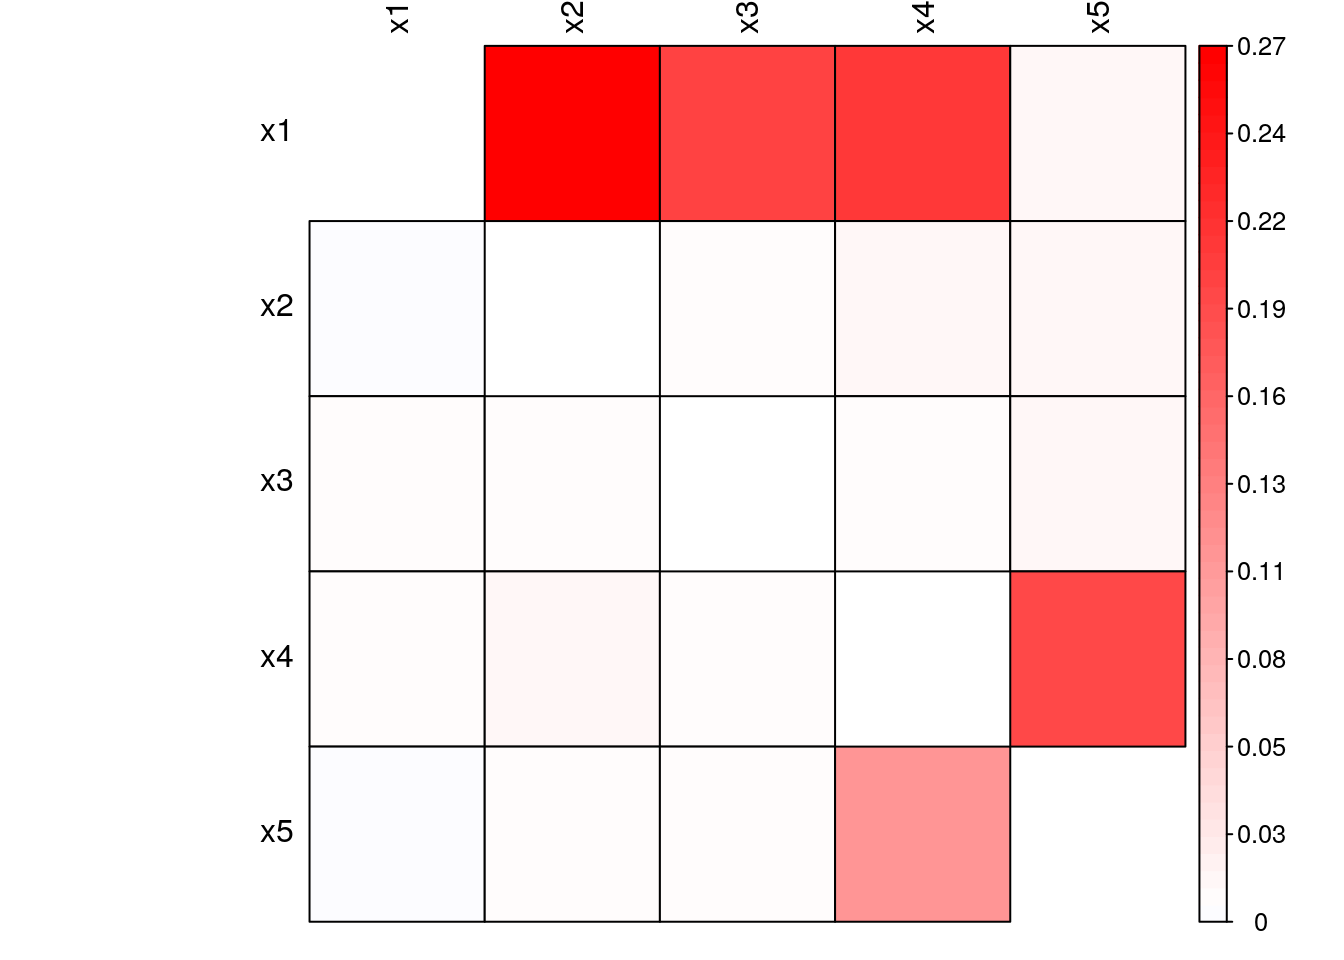
\includegraphics[width=1\linewidth]{open-quant-live-book_files/figure-latex/causality-graph-GC-1} 

}

\caption{Granger-Causality of simulated linear system}\label{fig:causality-graph-GC}
\end{figure}

\begin{figure}[H]

{\centering 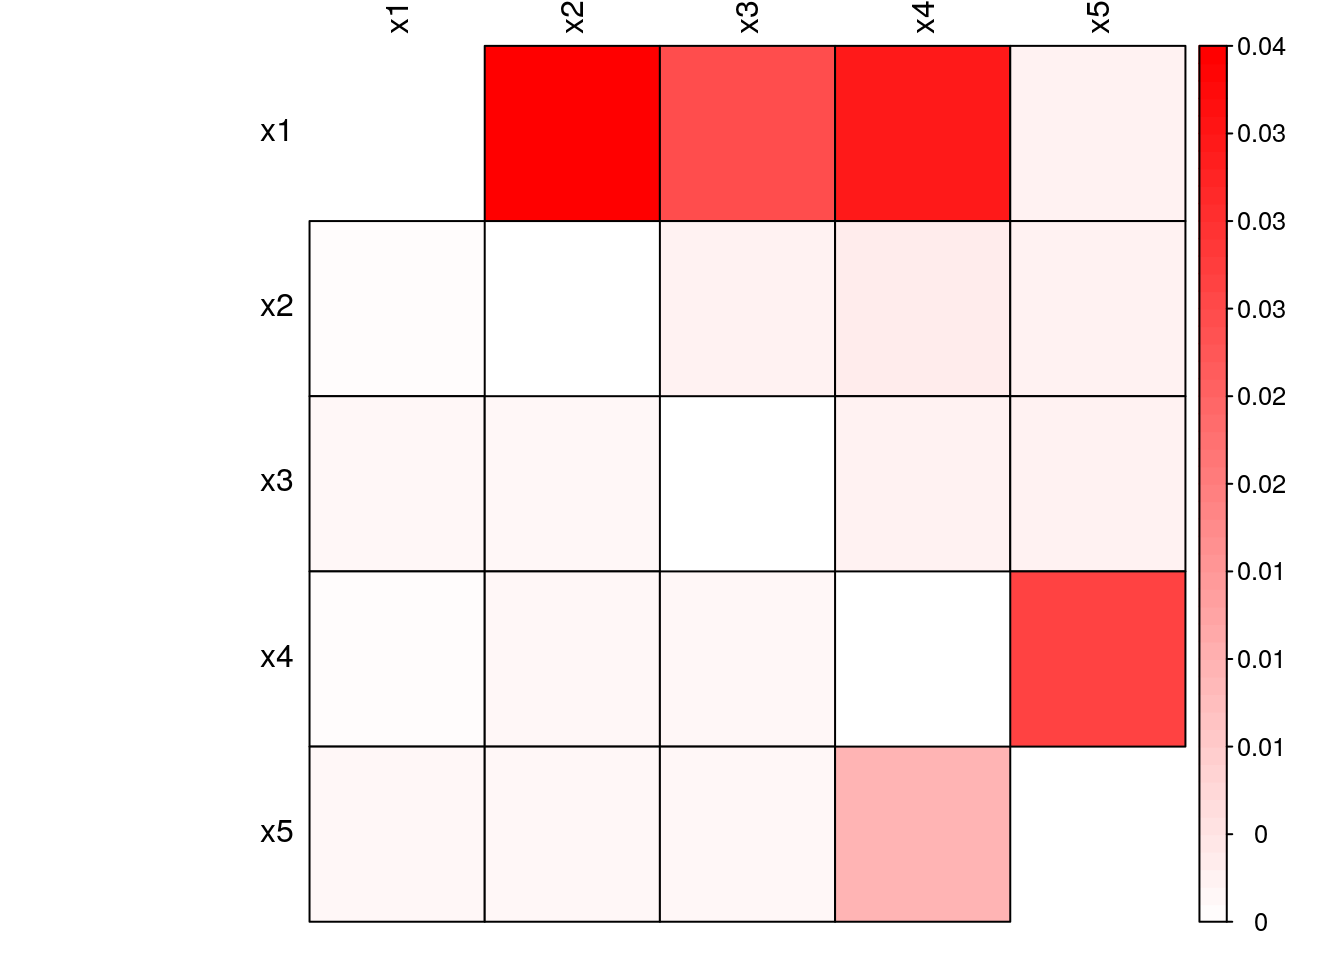
\includegraphics[width=1\linewidth]{open-quant-live-book_files/figure-latex/causality-graph-TE-1} 

}

\caption{Transfer Entropy of simulated linear system}\label{fig:causality-graph-TE}
\end{figure}

We define a second system by introducing nonlinear interactions between
\(x_1\) and the variables \(x_2\) and \(x_5\) as follows:

\begin{align}
x_1(n) &= 0.95\sqrt{2}x_1(n-1) - 0.9025x_1(n-1) + w_1\\ \nonumber
x_2(n) &= 0.5x_1^2(n-1) + w_2\\ \nonumber
x_3(n) &= -0.4x_1(n-1) + w_3\\ \nonumber
x_4(n) &= -0.5x_1^2(n-1) + 0.25\sqrt{2}x_4(n-1) + 0.25\sqrt{2}x_5(n-1) + w_4\\ \nonumber
x_5(n) &= -0.25\sqrt{2}x_4(n-1) + 0.25\sqrt{2}x_5(n-1) + w_5, \nonumber
\end{align}

where \(w_1, w_2, w_3, w_4\) and \(w_5 \sim N(0, 1)\). To simulate this
system we assume \(x_i(0) = 0, i \in (1, 2, ..., 5)\) as initial
condition and then iteratively generate \(x_i\) for
\(n \in (1, 2, ..., N)\) with a total of \(N = 10,000\) iterations by
randomly sampling \(w_i, i \in (1, 2, ..., 5)\) from a normal
distribution with zero mean and unit variance.

We simulate this nonlinear system with the following code:

\begin{Shaded}
\begin{Highlighting}[]
\KeywordTok{set.seed}\NormalTok{(}\DecValTok{123}\NormalTok{)}
\NormalTok{n <-}\StringTok{ }\DecValTok{10000}
\NormalTok{x1 <-}\StringTok{ }\NormalTok{x2 <-}\StringTok{ }\NormalTok{x3 <-}\StringTok{ }\NormalTok{x4 <-}\StringTok{ }\NormalTok{x5 <-}\StringTok{ }\KeywordTok{rep}\NormalTok{(}\DecValTok{0}\NormalTok{, n }\OperatorTok{+}\StringTok{ }\DecValTok{1}\NormalTok{)}

\ControlFlowTok{for}\NormalTok{ (i }\ControlFlowTok{in} \DecValTok{2}\OperatorTok{:}\NormalTok{(n }\OperatorTok{+}\StringTok{ }\DecValTok{1}\NormalTok{)) \{}
\NormalTok{  x1[i] <-}\StringTok{ }\FloatTok{0.95} \OperatorTok{*}\StringTok{ }\KeywordTok{sqrt}\NormalTok{(}\DecValTok{2}\NormalTok{) }\OperatorTok{*}\StringTok{ }\NormalTok{x1[i }\OperatorTok{-}\StringTok{ }\DecValTok{1}\NormalTok{] }\OperatorTok{-}\StringTok{ }\FloatTok{0.9025} \OperatorTok{*}\StringTok{ }\NormalTok{x1[i }\OperatorTok{-}\StringTok{ }
\StringTok{    }\DecValTok{1}\NormalTok{] }\OperatorTok{+}\StringTok{ }\KeywordTok{rnorm}\NormalTok{(}\DecValTok{1}\NormalTok{, }\DataTypeTok{mean =} \DecValTok{0}\NormalTok{, }\DataTypeTok{sd =} \DecValTok{1}\NormalTok{)}
\NormalTok{  x2[i] <-}\StringTok{ }\FloatTok{0.5} \OperatorTok{*}\StringTok{ }\NormalTok{x1[i }\OperatorTok{-}\StringTok{ }\DecValTok{1}\NormalTok{]}\OperatorTok{^}\DecValTok{2} \OperatorTok{+}\StringTok{ }\KeywordTok{rnorm}\NormalTok{(}\DecValTok{1}\NormalTok{, }\DataTypeTok{mean =} \DecValTok{0}\NormalTok{, }\DataTypeTok{sd =} \DecValTok{1}\NormalTok{)}
\NormalTok{  x3[i] <-}\StringTok{ }\OperatorTok{-}\FloatTok{0.4} \OperatorTok{*}\StringTok{ }\NormalTok{x1[i }\OperatorTok{-}\StringTok{ }\DecValTok{1}\NormalTok{] }\OperatorTok{+}\StringTok{ }\KeywordTok{rnorm}\NormalTok{(}\DecValTok{1}\NormalTok{, }\DataTypeTok{mean =} \DecValTok{0}\NormalTok{, }\DataTypeTok{sd =} \DecValTok{1}\NormalTok{)}
\NormalTok{  x4[i] <-}\StringTok{ }\OperatorTok{-}\FloatTok{0.5} \OperatorTok{*}\StringTok{ }\NormalTok{x1[i }\OperatorTok{-}\StringTok{ }\DecValTok{1}\NormalTok{]}\OperatorTok{^}\DecValTok{2} \OperatorTok{+}\StringTok{ }\FloatTok{0.25} \OperatorTok{*}\StringTok{ }\KeywordTok{sqrt}\NormalTok{(}\DecValTok{2}\NormalTok{) }\OperatorTok{*}\StringTok{ }\NormalTok{x4[i }\OperatorTok{-}\StringTok{ }
\StringTok{    }\DecValTok{1}\NormalTok{] }\OperatorTok{+}\StringTok{ }\FloatTok{0.25} \OperatorTok{*}\StringTok{ }\KeywordTok{sqrt}\NormalTok{(}\DecValTok{2}\NormalTok{) }\OperatorTok{*}\StringTok{ }\NormalTok{x5[i }\OperatorTok{-}\StringTok{ }\DecValTok{1}\NormalTok{] }\OperatorTok{+}\StringTok{ }\KeywordTok{rnorm}\NormalTok{(}\DecValTok{1}\NormalTok{, }\DataTypeTok{mean =} \DecValTok{0}\NormalTok{, }
    \DataTypeTok{sd =} \DecValTok{1}\NormalTok{)}
\NormalTok{  x5[i] <-}\StringTok{ }\OperatorTok{-}\FloatTok{0.25} \OperatorTok{*}\StringTok{ }\KeywordTok{sqrt}\NormalTok{(}\DecValTok{2}\NormalTok{) }\OperatorTok{*}\StringTok{ }\NormalTok{x4[i }\OperatorTok{-}\StringTok{ }\DecValTok{1}\NormalTok{] }\OperatorTok{+}\StringTok{ }\FloatTok{0.25} \OperatorTok{*}\StringTok{ }\KeywordTok{sqrt}\NormalTok{(}\DecValTok{2}\NormalTok{) }\OperatorTok{*}\StringTok{ }
\StringTok{    }\NormalTok{x5[i }\OperatorTok{-}\StringTok{ }\DecValTok{1}\NormalTok{] }\OperatorTok{+}\StringTok{ }\KeywordTok{rnorm}\NormalTok{(}\DecValTok{1}\NormalTok{, }\DataTypeTok{mean =} \DecValTok{0}\NormalTok{, }\DataTypeTok{sd =} \DecValTok{1}\NormalTok{)}
\NormalTok{\}}

\NormalTok{x1 <-}\StringTok{ }\NormalTok{x1[}\OperatorTok{-}\DecValTok{1}\NormalTok{]}
\NormalTok{x2 <-}\StringTok{ }\NormalTok{x2[}\OperatorTok{-}\DecValTok{1}\NormalTok{]}
\NormalTok{x3 <-}\StringTok{ }\NormalTok{x3[}\OperatorTok{-}\DecValTok{1}\NormalTok{]}
\NormalTok{x4 <-}\StringTok{ }\NormalTok{x4[}\OperatorTok{-}\DecValTok{1}\NormalTok{]}
\NormalTok{x5 <-}\StringTok{ }\NormalTok{x5[}\OperatorTok{-}\DecValTok{1}\NormalTok{]}
\NormalTok{nonlinear.system <-}\StringTok{ }\KeywordTok{data.frame}\NormalTok{(x1, x2, x3, x4, x5)}
\end{Highlighting}
\end{Shaded}

Fig. \ref{fig:C3S4Fig2} represents the dependencies of the simulated
nonlinear system.

\begin{figure}[H]

{\centering 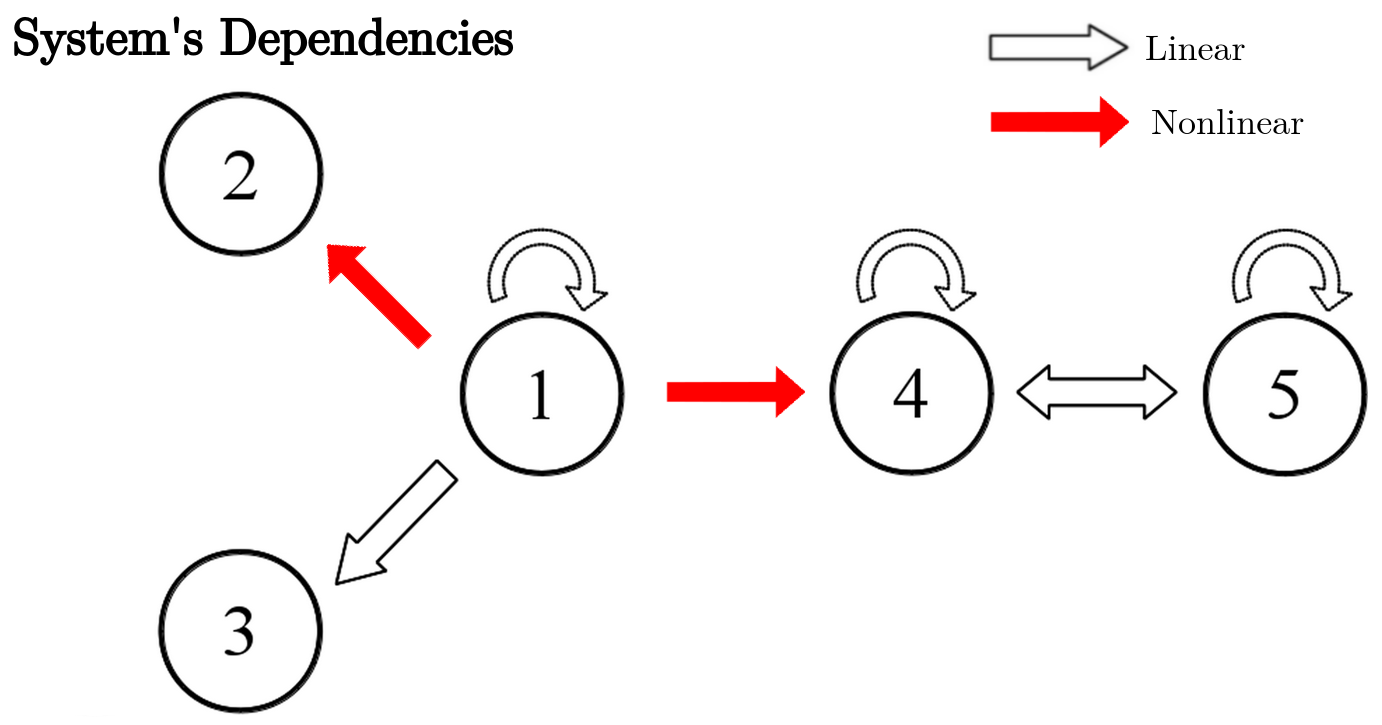
\includegraphics[width=1\linewidth]{./chapters/TransferEntropy/S4Fig2} 

}

\caption{Interactions between the variables of the simulated nonlinear system.}\label{fig:C3S4Fig2}
\end{figure}

We calculate Granger-causality and Transfer Entropy of the simulated
nonlinear system as follows:

\begin{Shaded}
\begin{Highlighting}[]
\NormalTok{## Allow for parallel computing}
\KeywordTok{plan}\NormalTok{(multiprocess)}


\NormalTok{## Calculates GC and TE}
\NormalTok{GC.matrix.nonlinear <-}\StringTok{ }\KeywordTok{FApply.Pairwise}\NormalTok{(nonlinear.system, }
\NormalTok{  Linear.GC)}
\NormalTok{TE.matrix.nonlinear <-}\StringTok{ }\KeywordTok{FApply.Pairwise}\NormalTok{(nonlinear.system, }
\NormalTok{  calc_te)}

\KeywordTok{rownames}\NormalTok{(TE.matrix.nonlinear) <-}\StringTok{ }\KeywordTok{colnames}\NormalTok{(TE.matrix.nonlinear) <-}\StringTok{ }\NormalTok{var.names}
\KeywordTok{rownames}\NormalTok{(GC.matrix.nonlinear) <-}\StringTok{ }\KeywordTok{colnames}\NormalTok{(GC.matrix.nonlinear) <-}\StringTok{ }\NormalTok{var.names}

\NormalTok{## Back to sequential computing}
\KeywordTok{plan}\NormalTok{(sequential)}
\end{Highlighting}
\end{Shaded}

From Fig. \ref{fig:causality-graph-nonlinear-GC} and Fig.
\ref{fig:causality-graph-nonlinear-TE}, we observe that the nonlinear
interactions introduced were not captured by the linear form of the
information flow. While all linear interactions presented similar linear
and nonlinear information flows, the two nonlinear interactions
introduced in the system presented relatively higher nonlinear
information flow compared to the linear formulation.

\begin{figure}[H]

{\centering 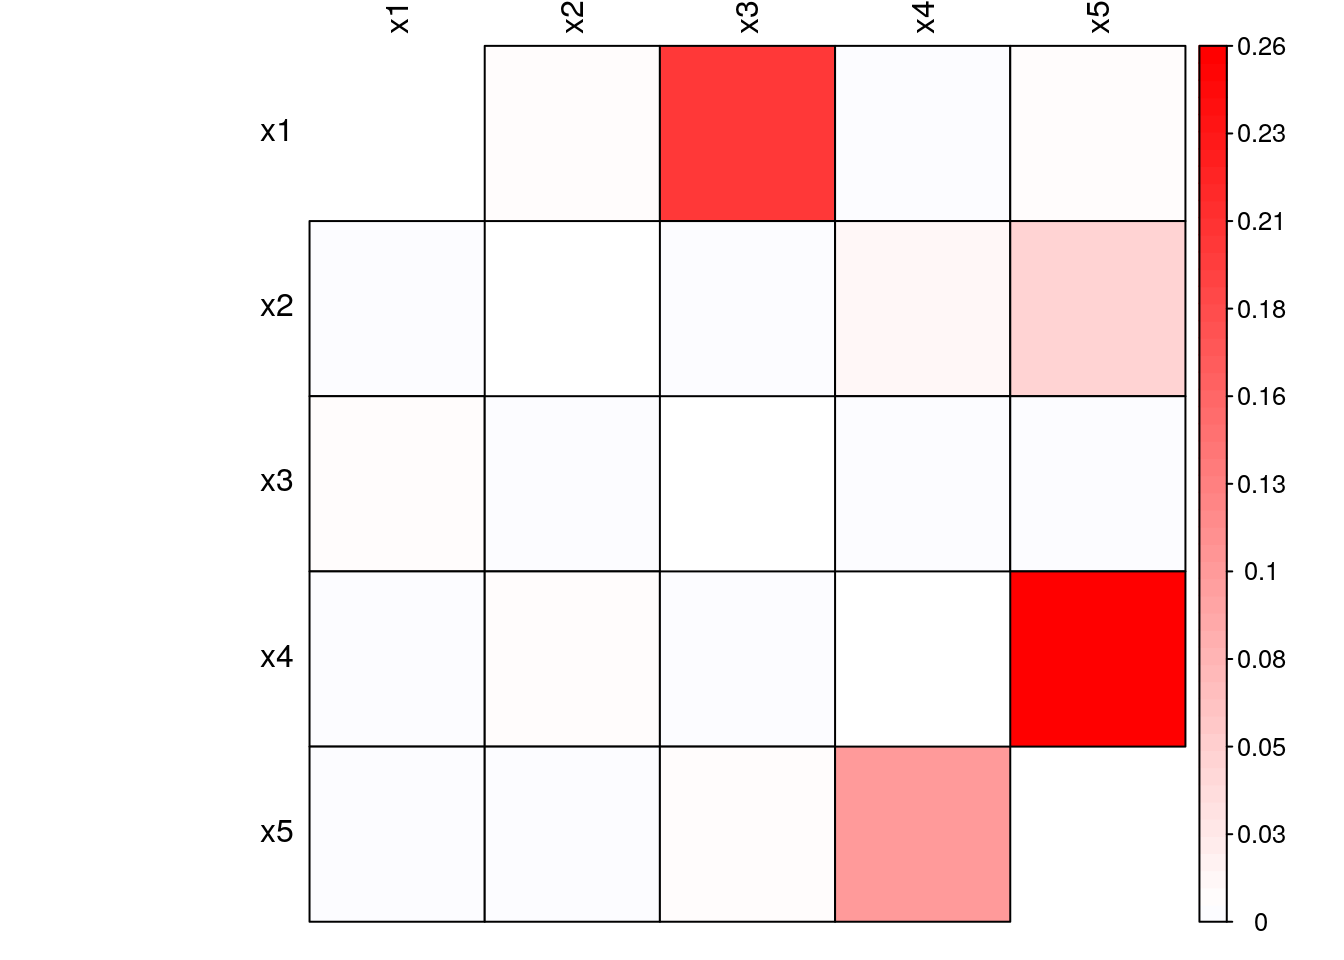
\includegraphics[width=1\linewidth]{open-quant-live-book_files/figure-latex/causality-graph-nonlinear-GC-1} 

}

\caption{Granger-Causality of simulated nonlinear system}\label{fig:causality-graph-nonlinear-GC}
\end{figure}

\begin{figure}[H]

{\centering 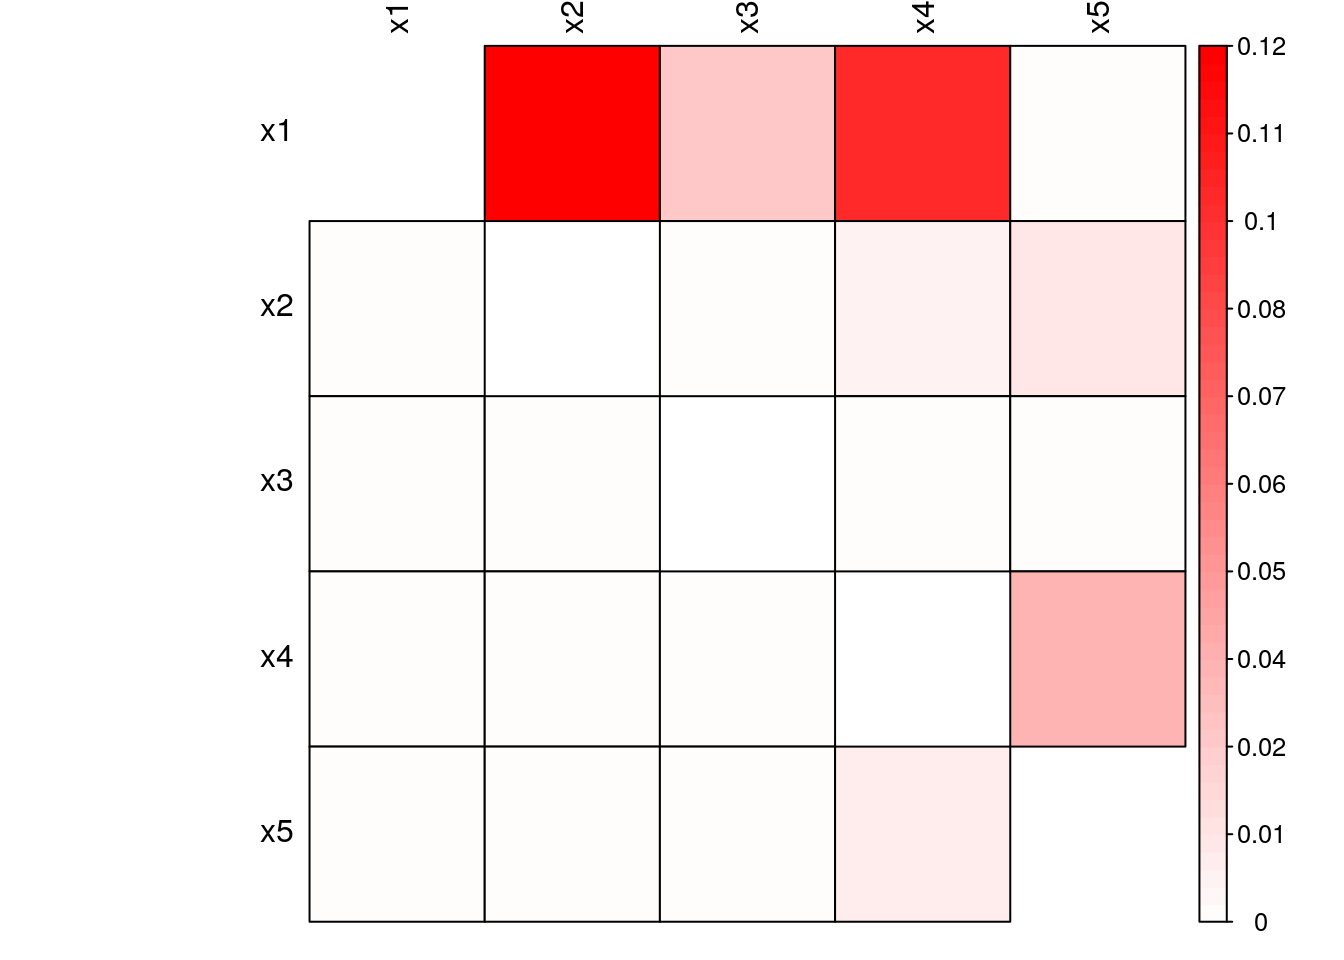
\includegraphics[width=1\linewidth]{open-quant-live-book_files/figure-latex/causality-graph-nonlinear-TE-1} 

}

\caption{Transfer Entropy of simulated nonlinear system}\label{fig:causality-graph-nonlinear-TE}
\end{figure}

\section{Information Flow among International Stock Market
Indices}\label{information-flow-among-international-stock-market-indices}

The world's financial markets form a complex, dynamic network in which
individual markets interact with one another. This multitude of
interactions can lead to highly significant and unexpected effects, and
it is vital to understand precisely how various markets around the world
influence one another \citep{junior2015dependency}.

In this section, we use Transfer Entropy for the identification of
dependency relations among international stock market indices. First, we
select some of the \href{https://finance.yahoo.com/world-indices/}{major
global indices} for our analysis, namely the S\&P 500, the FTSE 100, the
DAX, the EURONEXT 100 and the IBOVESPA, which track the following
markets, respectively, the US, the UK, Germany, Europe and Brazil. They
are defined by the following tickers:

\begin{Shaded}
\begin{Highlighting}[]
\NormalTok{tickers <-}\StringTok{ }\KeywordTok{c}\NormalTok{(}\StringTok{"^GSPC"}\NormalTok{, }\StringTok{"^FTSE"}\NormalTok{, }\StringTok{"^GDAXI"}\NormalTok{, }\StringTok{"^N100"}\NormalTok{, }\StringTok{"^BVSP"}\NormalTok{)}
\end{Highlighting}
\end{Shaded}

Next, we will load log-returns of daily closing adjusted prices for the
selected indices as follows (see Appendix \ref{dt-indices} for code used
to generate this dataset):

\begin{Shaded}
\begin{Highlighting}[]
\KeywordTok{library}\NormalTok{(xts)}
\NormalTok{dataset <-}\StringTok{ }\KeywordTok{as.xts}\NormalTok{(}\KeywordTok{read.zoo}\NormalTok{(}\StringTok{"./data/global_indices_returns.csv"}\NormalTok{, }
  \DataTypeTok{header =} \OtherTok{TRUE}\NormalTok{, }\DataTypeTok{index.column =} \DecValTok{1}\NormalTok{, }\DataTypeTok{sep =} \StringTok{","}\NormalTok{))}
\KeywordTok{head}\NormalTok{(dataset)}
\end{Highlighting}
\end{Shaded}

\begin{verbatim}
##                        X.GSPC   X.FTSE  X.GDAXI
## 2000-01-02 19:00:00  0.000000       NA  0.00000
## 2000-01-03 19:00:00 -0.039099  0.00000 -0.02456
## 2000-01-04 19:00:00  0.001920 -0.01969 -0.01297
## 2000-01-05 19:00:00  0.000955 -0.01366 -0.00418
## 2000-01-06 19:00:00  0.026730  0.00889  0.04618
## 2000-01-09 19:00:00  0.011128  0.01570  0.02109
##                       X.N100   X.BVSP
## 2000-01-02 19:00:00  0.00000  0.00000
## 2000-01-03 19:00:00 -0.04179 -0.06585
## 2000-01-04 19:00:00 -0.02726  0.02455
## 2000-01-05 19:00:00 -0.00842 -0.00853
## 2000-01-06 19:00:00  0.02296  0.01246
## 2000-01-09 19:00:00  0.01716  0.04279
\end{verbatim}

The influence that one market plays in another is dynamic. Here, we will
consider the time period from 01/01/2014 until today and we will omit
days with invalid returns due to bad data using the function
\texttt{NARV.omit} from the package \textbf{IDPmisc} as follows:

\begin{Shaded}
\begin{Highlighting}[]
\KeywordTok{library}\NormalTok{(IDPmisc)}
\NormalTok{dataset.post.crisis <-}\StringTok{ }\KeywordTok{NaRV.omit}\NormalTok{(}\KeywordTok{as.data.frame}\NormalTok{(dataset[}\StringTok{"2014-01-01/"}\NormalTok{]))}
\end{Highlighting}
\end{Shaded}

We will calculate pairwise Transfer Entropy among all indices considered
and construct a matrix such that each value in the position \((i,j)\)
will contain the value Transfer Entropy from \(tickers[i]\) to
\(tickers[j]\) as follows:

\begin{Shaded}
\begin{Highlighting}[]
\NormalTok{## Allow for parallel computing}
\KeywordTok{plan}\NormalTok{(multiprocess)}

\CommentTok{# Calculate pairwise Transfer Entropy among global}
\CommentTok{# indices}
\NormalTok{TE.matrix <-}\StringTok{ }\KeywordTok{FApply.Pairwise}\NormalTok{(dataset.post.crisis, calc_ete)}
\KeywordTok{rownames}\NormalTok{(TE.matrix) <-}\StringTok{ }\KeywordTok{colnames}\NormalTok{(TE.matrix) <-}\StringTok{ }\NormalTok{tickers}

\NormalTok{## Back to sequential computing}
\KeywordTok{plan}\NormalTok{(sequential)}
\end{Highlighting}
\end{Shaded}

Fig. \ref{fig:TEmatrix} displays the resulting Transfer Entropy matrix.
We normalize the Transfer Entropy values by dividing it by the maximum
value in the matrix such that all values range from 0 to 1. We observe
that the international indices studied are highly interconnected in the
period analyzed with the highest information flow going from the US
market to the UK market (\^{}GSPC -\textgreater{} \^{}FTSE). The second
highest information flow is going from the UK market to the US market.
That's a result we would expect as the US and the UK markets are
strongly coupled, historically.

\begin{figure}[H]

{\centering 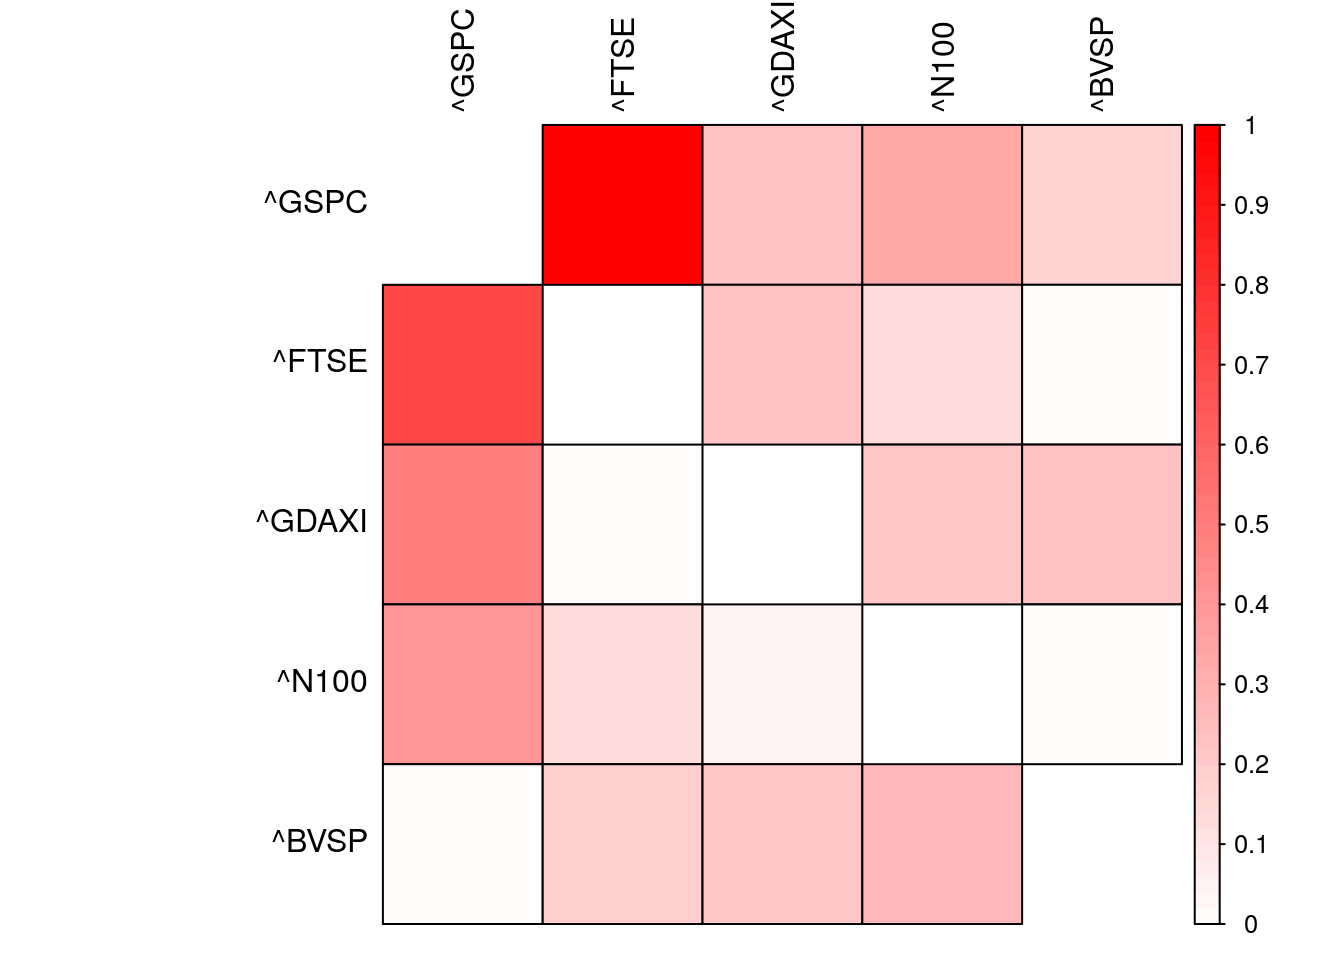
\includegraphics[width=1\linewidth]{open-quant-live-book_files/figure-latex/TEmatrix-1} 

}

\caption{Normalized Transfer Entropy among international stock market indices.}\label{fig:TEmatrix}
\end{figure}

We also calculate the marginal contribution of each market to the total
Transfer Entropy in the system by calculating the sum of Transfer
Entropy for each row in the Transfer Entropy matrix, which we also
normalize such that all values range from 0 to 1:

\begin{Shaded}
\begin{Highlighting}[]
\NormalTok{TE.marginal <-}\StringTok{ }\NormalTok{base}\OperatorTok{::}\KeywordTok{apply}\NormalTok{(TE.matrix, }\DecValTok{1}\NormalTok{, sum)}
\NormalTok{TE.marginal.norm <-}\StringTok{ }\NormalTok{TE.marginal}\OperatorTok{/}\KeywordTok{sum}\NormalTok{(TE.marginal)}
\KeywordTok{print}\NormalTok{(TE.marginal.norm)}
\end{Highlighting}
\end{Shaded}

\begin{verbatim}
##  ^GSPC  ^FTSE ^GDAXI  ^N100  ^BVSP 
##  0.346  0.215  0.187  0.117  0.135
\end{verbatim}

We observe that the US is the most influential market in the time period
studied detaining 34.632\% of the total Transfer Entropy followed by the
UK and Germany with 21.472\% and 18.653\%, respectively. Japan and
Brazil are the least influential markets with normalized Transfer
Entropies of 11.744\% and 13.498\%, respectively.

An experiment left to the reader is to build a daily trading strategy
that exploits information flow among international markets. The proposed
thesis is that one could build a profitable strategy by placing bets on
futures of market indices that receive significant information flow from
markets that observed unexpected returns/movements.

For an extended analysis with a broader set of indices see
\citep{junior2015dependency}. The authors develop networks of
international stock market indices using an information theoretical
framework. They use 83 stock market indices of a diversity of countries,
as well as their single day lagged values, to probe the correlation and
the flow of information from one stock index to another taking into
account different operating hours. They find that Transfer Entropy is an
effective way to quantify the flow of information between indices, and
that a high degree of information flow between indices lagged by one day
coincides to same day correlation between them.

\section{Other Applications}\label{other-applications}

\subsection{Quantifying Information Flow Between Social Media and the
Stock
Market}\label{quantifying-information-flow-between-social-media-and-the-stock-market}

Investors' decisions are modulated not only by companies' fundamentals
but also by personal beliefs, peers influence and information generated
from news and the Internet. Rational and irrational investor's behavior
and their relation with the market efficiency hypothesis
\citep{JOFI:JOFI518} have been largely debated in the economics and
financial literature \citep{shleifer2000inefficient}. However, it was
only recently that the availability of vast amounts of data from online
systems paved the way for the large-scale investigation of investor's
collective behavior in financial markets.

A research paper \citep{2016arXiv160104535S} used some of the methods
studied in this Chapter to uncover that information flows from social
media to stock markets revealing that tweets are causing market
movements through a nonlinear complex interaction. The authors provide
empirical evidence that suggests social media and stock markets have a
nonlinear causal relationship. They take advantage of an extensive data
set composed of social media messages related to DJIA index components.
By using information-theoretic measures to cope for possible nonlinear
causal effects between social media and the stock market, the work
points out stunning differences in the results with respect to linear
coupling. Two main conclusions are drawn: First, social media
significant causality on stocks' returns are purely nonlinear in most
cases; Second, social media dominates the directional coupling with
stock market, an effect not observable within linear modeling. Results
also serve as empirical guidance on model adequacy in the investigation
of sociotechnical and financial systems.

Fig. \ref{fig:sigpoints-0} shows the significant causality links found
between social media and stocks' returns considering both cases:
nonlinear (Transfer Entropy) and linear G-causality (linear VAR
framework). The linear analysis discovers only three stocks with
significant causality: INTEL CORP., NIKE INC. and WALT DISNEY CO. The
Nonlinear analysis discovers that several other stocks have significant
causality. In addition to the 3 stocks identified with significant
linear causality, other 8 stocks presented purely nonlinear causality.

\begin{figure}[H]

{\centering 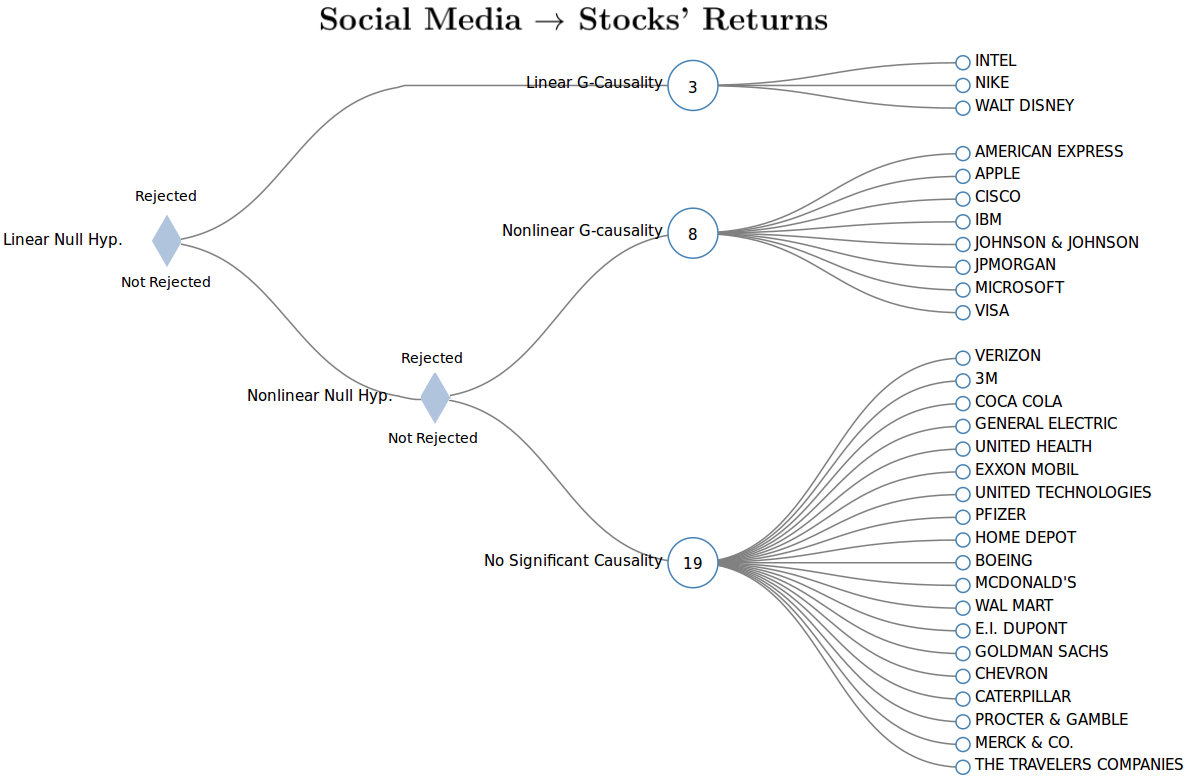
\includegraphics[width=1\linewidth]{./chapters/TransferEntropy/SM-R-33} 

}

\caption{Demonstration that the causality between social media and stocks' returns are mostly nonlinear. Linear causality test indicated that social media caused stock's returns only for 3 stocks. Nonparametric analysis showed that almost 1/3 of the stocks rejected in the linear case have significant nonlinear causality. In the nonlinear case, Transfer Entropy was used to quantify causal inference between the systems with randomized permutations test for significance estimation. In the linear case, a standard linear G-causality test was performed with a F-test under a linear vector-autoregressive framework. A significant linear G-causality was accepted if its linear specification was not rejected by the BDS test. p-values are adjusted with the Bonferroni correction. Significance is given at p-value  < 0.05.}\label{fig:sigpoints-0}
\end{figure}

The low level of causality obtained under linear constraints is in-line
with results from similar studies in the literature, where it was found
that stocks' returns show weak causality links
\citep[\citet{Antweiler+Frank:04a}]{Tobias:2013} and social media
sentiment analytics, at least when taken alone, have small or no
predictive power \citep{10.1371/journal.pone.0138441} and do not have
significant lead-time information about stock's movements for the
majority of the stocks \citep{citeulike:13108056}. Contrariwise, results
from the nonlinear analyses unveiled a much higher level of causality
indicating that linear constraints may be neglecting the relationship
between social media and stock markets.

In summary, this paper \citep{2016arXiv160104535S} is a good example on
how causality can be not only complex but also misleading further
highlighting the importance of choice in the methodology used to
quantify it.

\subsection{Detecting Causal Links Between Investor Sentiment and
Cryptocurrency
Prices}\label{detecting-causal-links-between-investor-sentiment-and-cryptocurrency-prices}

In \citep{keskin2019information}, the authors use information-theoretic
measures studied in this Chapter for non-linear causality detection
applied to social media sentiment and cryptocurrency prices.

Using these techniques on sentiment and price data over a 48-month
period to August 2018, for four major cryptocurrencies, namely bitcoin
(BTC), ripple (XRP), litecoin (LTC) and ethereum (ETH), the authors
detect significant information transfer, on hourly timescales, in
directions of both sentiment to price and of price to sentiment. The
work reports the scale of non-linear causality to be an order of
magnitude greater than linear causality.

The information-theoretic investigation detected a significant
non-linear causal relationship in BTC, LTC and XRP, over multiple
timescales and in both the directions sentiment to price and price to
sentiment. The effect was strongest and most consistent for BTC and LTC.
Fig. \ref{fig:te-crypto} shows Transfer Entropy results between BTC
sentiment and BTC prices.

\begin{figure}[H]

{\centering 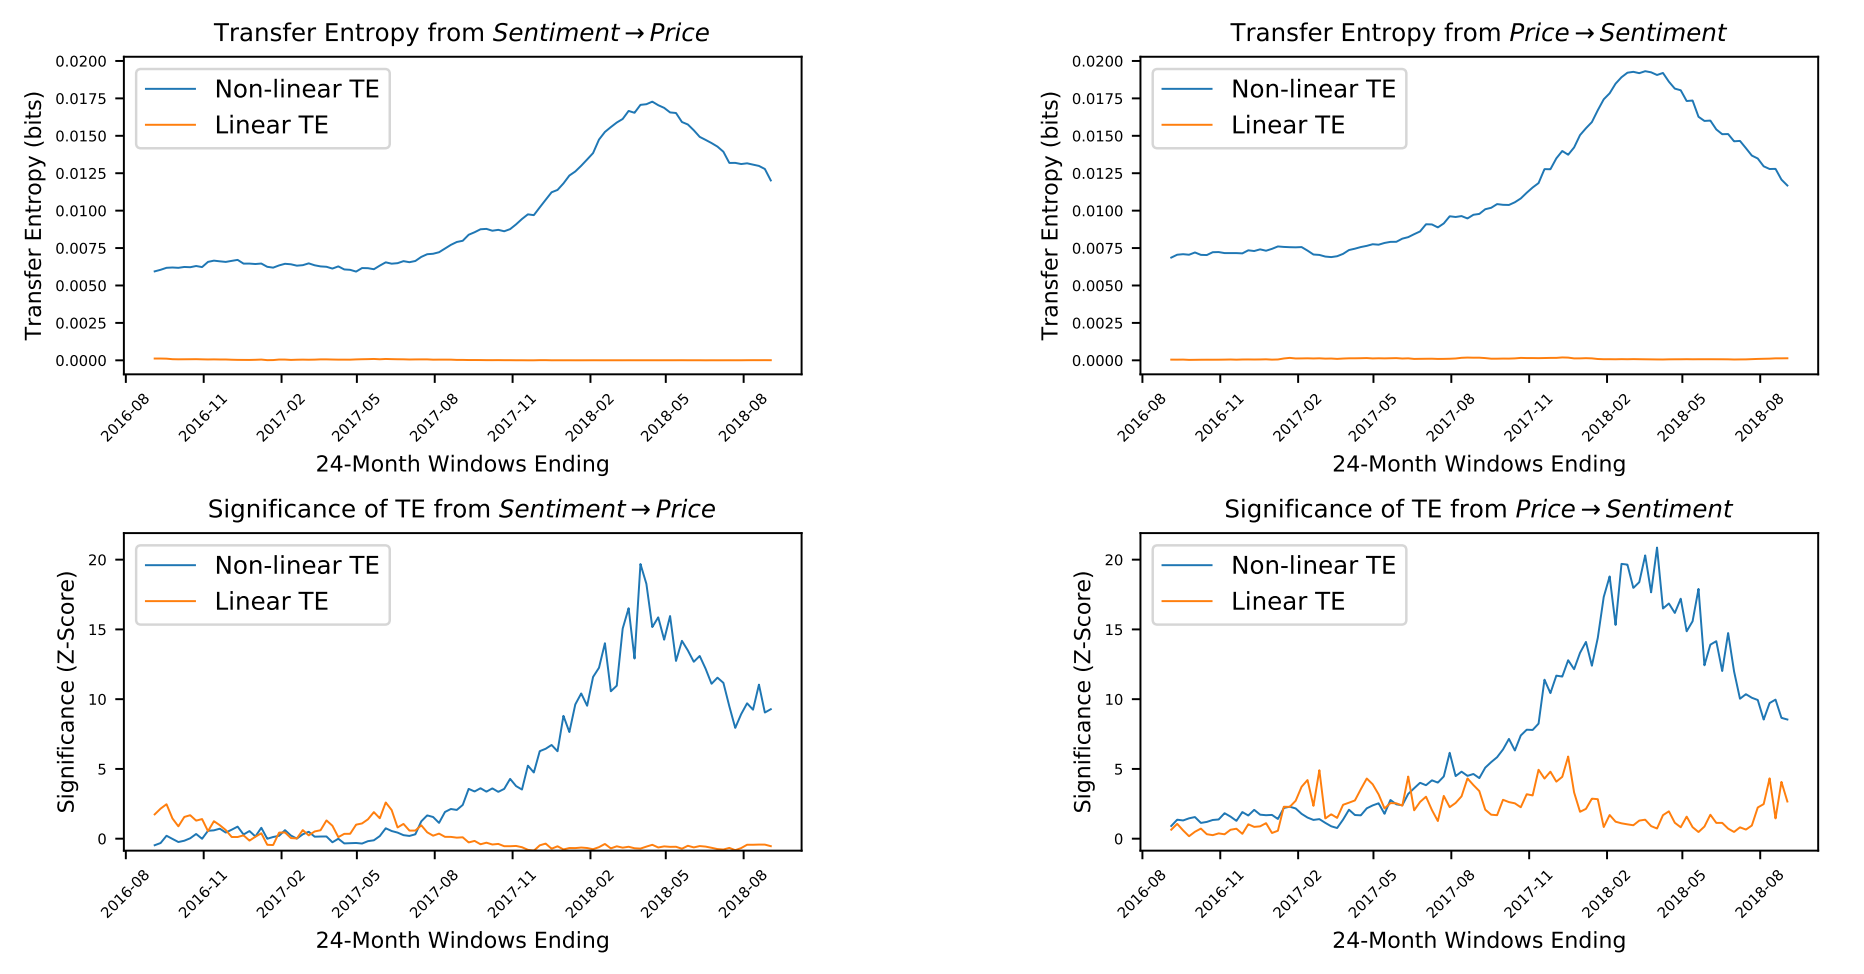
\includegraphics[width=1\linewidth]{./chapters/TransferEntropy/te-crypto} 

}

\caption{Evidence that BTC sentiment and price are causally coupled in both directions in a non-linear way. Non-linear TE is calculated by multidimensional histograms with 6 quantile bins per dimension. Z-scores, calculated over 50 shuffles, show a high level of significance, especially during 2017 and 2018, in both directions.}\label{fig:te-crypto}
\end{figure}

All analysis for this paper was performed using a Python package
(PyCausality), which is available at
\url{https://github.com/ZacKeskin/PyCausality}.

\section{Conclusions}\label{conclusions}

Untangling cause and effect can be devilishly difficult. However,
statistical tools can help us tell correlation from causation.

In this Chapter, we introduced the notion of Granger-causality and its
traditional implementation in a linear vector-autoregressive framework.
We then defined information theoretical measures to quantify Transfer
Entropy as a method to estimate statistical causality in nonlinear
systems.

We simulated linear and nonlinear systems further showing that the
traditional linear G-causality approach failed to detect simple
non-linearities introduced into the system while Transfer Entropy
successfully detected such relationships.

Finally, we showed how Transfer Entropy can be used to quantify
relationships among global equity indexes. We also discussed further
applications from the literature where Information Theoretical measures
were used to quantify causal links between investor sentiment and
movements in the equity and crypto markets.

We hope you enjoyed this casual causal journey and remember: Quantify
causality, responsibly.

\chapter{Financial Networks}\label{financial-networks}

\section{Introduction}\label{introduction-2}

Financial markets can be regarded as a complex network in which nodes
represent different financial assets and edges represent one or many
types of relationships among those assets. Filtered correlation-based
networks have successfully been used in the literature to study
financial markets structure particularly from observational data derived
from empirical financial time series
\citep[\citet{Tumminello26072005}]{bardoscia2017pathways, 10.1371/journal.pone.0017994, Mantegna1999, aste2010correlation, Tumminello201040}.

The underlying principle is to use correlations from empirical financial
time series to construct a sparse network representing the most relevant
connections. Analyses on filtered correlation-based networks for
information extraction \citep{song2008analysis, aste2010correlation}
have widely been used to explain market interconnectedness from
high-dimensional data. Applications include asset allocation
\citep{LI2018, pozzi2013spread}, market stability assessments
\citep{morales2012dynamical}, hierarchical structure analyses
\citep{Mantegna1999, aste2010correlation, Tumminello201040, musmeci2014clustering, song2012hierarchical}
and the identification of lead-lag relationships
\citep{curme2015coupled}.

In this Chapter we will describe how to

\begin{itemize}
\tightlist
\item
  Construct and filter financial networks;
\item
  Build price-based dynamic industry taxonomies;
\item
  Implement a trading strategy based on financial network structure.
\end{itemize}

\section{Network Construction}\label{network-construction}

We selected \(N = 100\) of the most capitalized companies that were part
of the S\&P500 index from 09/05/2012 to 08/25/2017. The list of these
companies' ticker symbols is reported in the Appendix \ref{sec:comps}.
For each stock \(i\) the financial variable was defined as the daily
stock's log-return \(R_i(\tau)\) at time \(\tau\).

Stock returns \(R_i\) and social media opinion scores \(O_i\) each
amounted to a time series of length equals to 1251 trading days. These
series were divided time-wise into \(M = 225\) windows
\(t = 1, 2, \ldots, M\) of width \(T = 126\) trading days. A window step
length parameter of \(\delta T = 5\) trading days defined the
displacement of the window, i.e., the number of trading days between two
consecutive windows. The choice of window width \(T\) and window step
\(\delta T\) is arbitrary, and it is a trade-off between having analysis
that is either too dynamic or too smooth. The smaller the window width
and the larger the window steps, the more dynamic the data are.

To characterize the synchronous time evolution of assets, we used equal
time Kendall's rank coefficients between assets \(i\) and \(j\), defined
as

\begin{equation}
 \rho_{i, j}(t) = \sum\limits_{t' < \tau}sgn(V_i(t') - V_i(\tau))sgn(V_j(t') - V_j(\tau)),
\end{equation}

where \(t'\) and \(\tau\) are time indexes within the window \(t\) and
\(V_i \in \{R_i, O_i\}\).

Kendall's rank coefficients takes into account possible nonlinear
(monotonic) relationships. It fulfill the condition
\(-1 \leq \rho_{i, j} \leq 1\) and form the \(N \times N\) correlation
matrix \(C(t)\) that served as the basis for the networks constructed in
this work. To construct the asset-based financial and social networks,
we defined a distance between a pair of stocks. This distance was
associated with the edge connecting the stocks, and it reflected the
level at which they were correlated. We used a simple non-linear
transformation \(d_{i, j}(t) = \sqrt{2(1 - \rho_{i,j}(t))}\) to obtain
distances with the property \(2 \geq d_{i,j} \geq 0\), forming a
\(N \times N\) symmetric distance matrix \(D(t)\).

\subsection{Network Filtering: Asset
Graphs}\label{network-filtering-asset-graphs}

We extract the \(N(N-1)/2\) distinct distance elements from the upper
triangular part of the distance matrix \(D(t)\), which were then sorted
in an ascending order to form an ordered sequence
\(d_1(t), d_2(t), \ldots, d_{N(N-1)/2}(t)\). Since we require the graph
to be representative of the market, it is natural to build the network
by including only the strongest connections. This is a network filtering
procedure that has been successfully applied in the construction of
\textit{asset graphs} for the analyses of market structure
\cite{1402-4896-2003-T106-011, refId0-Onnela-2004}. The number of edges
to include is arbitrary, and we included those from the bottom quartile,
which represented the 25\% shortest edges in the graph (largest
correlations), thus giving
\(E(t) = \{d_1(t), d_2(t), \ldots, d_{\floor{N/4}}(t)\}\).

We denoted \(E^{F}(t)\) as the set of edges constructed from the
distance matrix derived from stock returns \(R(t)\). The financial
network considered is \(G^{F} = ( V, E^{F} )\), where \(V\) is the
vertex set of stocks.

\subsection{Network Filtering: MST}\label{network-filtering-mst}

\subsection{Network Filtering: PMFG}\label{network-filtering-pmfg}

\section{Applications}\label{applications}

\subsection{Industry Taxonomy}\label{industry-taxonomy}

\subsection{Portfolio Construction}\label{portfolio-construction}

\part{Alternative Data}\label{part-alternative-data}

\chapter{The Market, The Players and The
Rules}\label{the-market-the-players-and-the-rules}

\section{The Market}\label{the-market}

In an industry where almost every player has access to the same (or
similar) core financial and fundamental data, investment firms look for
Alternative Data seeking differentiated insights into companies not
found in filings, earnings calls or fundamental datasets.

Until recently, the usage of alternative data has been confined mainly
to the realm of quantitative investment managers, as these firms were
best suited to obtain, clean and process this data. Now, however,
alternative data is beginning to go mainstream, with increasing interest
from fundamental and hybrid asset managers here \citep{Greenwich_2019}.

\begin{quote}
\textbf{Alternative Data is Untapped Alpha.} The biggest opportunity for
investors in this decade comes from the signals buried in the data
generated by the digital economy. Alternative data is the deepest, least
utilized alpha source in the world today -
\href{www.quandl.com}{Quandl}.
\end{quote}

On June/2019, alternative data went mainstream when Verizon made a bold
move by launching a
\href{https://www.linkedin.com/feed/update/urn:li:activity:6544977248175349760}{subscription
service for Yahoo Finance} that offers alternative data and insights to
retail investors at a price point of \$34.99/month.

\begin{quote}
\textbf{The amount spent in Alternative Data have been steadily
increasing.} More than half of all quantitative and fundamental
investors surveyed recently are either considering or using alternative
data as part of their workflow -
\href{https://www.valuewalk.com/2019/07/alternative-data-paradigms-of-fundamental-and-quantitative/}{Greenwich
Associates}.
\end{quote}

A recent
\href{https://www.valuewalk.com/2019/07/alternative-data-paradigms-of-fundamental-and-quantitative/}{Greenwich
Associates report} found that a wide majority of investment managers,
72\%, stated that alternative data was improving enhanced their signal
quality in an arena where filtering out signal noise. Of those who are
implementing an alternative data strategy, more than one-fifth claim to
have received 20\% or more of their alpha from the practice.

\begin{figure}[h]

{\centering \includegraphics[width=1\linewidth]{https://cdn-images-1.medium.com/max/1600/0*GirclNZeAoiHWNne} 

}

\caption{Total Buy-side spend on Alternative Data has been steadily increasing and its likely to nearly triple from 2018 to 2020.}\label{fig:unnamed-chunk-59}
\end{figure}

\section{The Data}\label{the-data}

But where's Alternative Data coming from and who are the key players
providing access to it?

\begin{figure}[h]

{\centering \includegraphics[width=1\linewidth]{https://cdn-images-1.medium.com/max/1600/0*s_Pil2lOeWW6hJ_a} 

}

\caption{Alternative Data are sourced by heterogeneous sources including individuals, businesses and sensors.}\label{fig:unnamed-chunk-60}
\end{figure}

The growth of Alternative Data has been enabled by the digitalization of
the world around us. Data have been produced at an unprecedented rate by
heterogeneous sources including:

\begin{enumerate}
\def\labelenumi{\arabic{enumi}.}
\tightlist
\item
  Individuals who today mirror their lives in the form digital behavior
  into the Web, Social Media and Apps;
\item
  Sensors, particularly with the emergence of IoT, that generate
  satellite images, weather forecasts and geolocation data;
\item
  Businesses from which data is generated in the form of traditional
  official filings and earning calls as well as banking records or
  supply chain data.
\end{enumerate}

\begin{figure}[h]

{\centering \includegraphics[width=1\linewidth]{https://cdn-images-1.medium.com/max/1600/0*VsYQ_IxQ2EHp1w8B} 

}

\caption{The number of Alternative Data Providers is exploding.}\label{fig:unnamed-chunk-61}
\end{figure}

The number of Alternative Data Providers is exploding.The number of
alternative data vendors is exploding particularly in the past decade. A
few companies are worth mentioning:

\begin{enumerate}
\def\labelenumi{\arabic{enumi}.}
\tightlist
\item
  \href{https://www.quandl.com}{\textbf{Quandl}} is likely the largest
  financial and alternative data aggregator/provider today. They
  leverage relationships with third-party providers to be a
  one-stop-shop for alternative data from consumers, IoT and sentiment
  to traditional fundamental, pricing and estimates.
  \href{https://www.businessinsider.com/nasadaq-buys-alternative-data-firm-quandl-2018-12}{Quandl
  has been recently acquired by Nasdaq}.
\item
  \href{https://www.dataminr.com}{\textbf{Dataminr}} leverages advanced
  anomaly detection technology in a real-time AI platform to uncover
  critical events from social media before the information goes
  mainstream. The company raised a staggering \$500MM+ amount in funding
  so far and it gives no sign of that is slowing down.
\item
  \href{https://www.thinknum.com}{\textbf{Thinknum}} provides a
  SaaS-based web platform for a variety of alternative data sets, in
  particular, web-scrapped data such as product comparisons and company
  ratings on jobs sites. Thinkum claims to have 8 of the 10 largest
  investment banks as their clients. They recently closed a \$11.6
  million Series A funding to expand their financial modeling tools.
\item
  \href{https://www.yewno.com}{\textbf{Yewno}} is helping the world to
  uncover the undiscovered through its advanced dynamic Knowledge Graph
  and AI based inference engine, which introduces an entirely new
  approach to knowledge extraction to enhance human understanding by
  correlating concepts across a vast volume of sources. Yewno ingests
  data from sources such as clinical trials, patents, company
  transcripts and court opinions and more. Yewno raised about \$30
  million dollars in funding and it has launched AI-based equity indexes
  with major partners such as STOXX and Nasdaq and licensed alternative
  data feeds to buy-side firms.
\end{enumerate}

Other rising vendors include YipitData, 1010data and Enigma as well as
incumbent players such as Refinitiv, S\&P Global Market Intelligence,
Bloomberg and Factset.

\begin{quote}
While the alternative data offering is exploding there is a gap between
what data vendors offer and what data buyers want.
\end{quote}

A
\href{https://alternativedata.org/new-alternative-data-pricing-report/}{research}
report conducted by BattleFin and AlternativeData.org has found that
there is a gap between what data vendors offer and what data buyers
actually want: - Data buyers view the three most-valuable data
categories as: credit/debit cards (14.83\%) web data (12.29\%), and
social/sentiment (11.02\%). - By contrast, the percentage of data
providers covering these data categories are: credit card (0.69\%),
web-crawled data (3.94\%) and sentiment (4.40\%). - Data providers
report that the top-three categories their data covers are: business
insights (6.48\%), web traffic (4.63\%) and sentiment (4.40\%).

\begin{figure}[h]

{\centering \includegraphics[width=1\linewidth]{https://cdn-images-1.medium.com/max/1600/1*I9bxxOlaZu5s7Vk5AhnVXA} 

}

\caption{Data extracted from a research report conducted by BattleFin and AlternativeData.org, which compiles responses from 173 respondents made up of 69 alternative-data buyers and 104 data providers who responded to a 2018 survey conducted by BattleFin.}\label{fig:unnamed-chunk-62}
\end{figure}

\section{The Buyers}\label{the-buyers}

The data buyers include your usual suspects such as Two Sigma,
Milennium, Third Point, WorldQuant, ExodusPoint and emerging Quant Funds
like Credit Suisse's QT Fund.

\begin{quote}
\textbf{80\% of buyers expect to purchase} a minimum of one to five
datasets in 2019 while nearly 60 percent expects to test and evaluate a
minimum of one to five datasets this year - according to a
\href{https://alternativedata.org/new-alternative-data-pricing-report/}{research}
report conducted by BattleFin and AlternativeData.org.
\end{quote}

Pension Plans and Index Providers are also entering the space seeking
exposure to alternative factors, particularly with the emergence of
AI-based strategies that leverage machine learning and computational
linguistics techniques to extract signals from unstructured data (see
\href{https://medium.com/@souzatharsis/weve-launched-the-world-s-first-ai-index-9f9a6e931c58?source=friends_link\&sk=6d1e820e829669ad10097ac1f19b544c}{STOXX}'s
or
\href{https://medium.com/datadriveninvestor/ai-big-data-etf-ac6f7dda94d8}{DWS}'s
AI-based indexes) as well as the increased interest in themes such as
ESG (Environmental, Social and Corporate Governance) - a
multi-dimensional multi-sourced theme with increasing demands that are
no longer met by traditional data sources alone.

I have been to a good number of meetings with data buyers (BattleFin is
maybe the best event out there for 1-on-1 meetings with high-profile
buy-side firms sometimes allowing for 30+ meetings in two days of events
in addition to dozens of unofficial ones). Some questions are
commonplace:

\begin{enumerate}
\def\labelenumi{\arabic{enumi}.}
\tightlist
\item
  Can you describe your data sources and your data ingestion process?
\item
  What's the frequency/history/coverage?
\item
  What's the delivery method?
\item
  What are the key use cases for your data?
\item
  Can I run a trial with live data?
\item
  Who are your clients?
\item
  What's pricing like?
\item
  Do you offer exclusivity?
\item
  What is the size/funding/team profile of your firm?
\end{enumerate}

There is one tricky question though: Whether the data was already
licensed to other clients. Particularly if the buyer is looking for
alpha, they actually would prefer to be one of the first to test the
data and avoid using a dataset that is already ``crowded''. By the same
token, they would be happy to hear that the dataset was already licensed
to reputable clients as a sign of credibility. It's up to you to
navigate through this trade-off.

\begin{figure}[h]

{\centering \includegraphics[width=1\linewidth]{https://cdn-images-1.medium.com/max/1600/1*MRcgvpX8o1RT8HZwOr12jw} 

}

\caption{The sales life-cycle of an alternative data product can take up to seven months from lead generation to customer sign-up. Image by Quandl.}\label{fig:unnamed-chunk-63}
\end{figure}

This is just the very first step in the sales and marketing life-cycle.
From lead generation to customer sign-up, data buyers can take several
months to make a final decision. Here are some
\href{https://alternativedata.org/new-alternative-data-pricing-report/}{findings}:

\begin{enumerate}
\def\labelenumi{\arabic{enumi}.}
\tightlist
\item
  \textbf{Providers and buyers agree that alt-data sales cycle can take
  up to seven months}, with more than 75\% of buyers requiring up to six
  months to test, evaluate and purchase an alt dataset.
\item
  \textbf{More than a third of data buyers use backtesting} to inform
  their purchasing decision. Nearly 60\% of providers are not interested
  in outsourcing the data testing process even if it can be handled
  efficiently.
\item
  \textbf{More than 20\% of providers sell and distribute using a
  customized alt-data software platform.} Nearly 18\% use no software
  platform at all.
\end{enumerate}

\section{Conclusion}\label{conclusion-1}

Alternative Data, once a treat only for the most advanced Hedge Funds,
is becoming a must-have in the alpha-generation war on Wall Street.

Total spending in the area has been steadily growing as well as the
number of data vendors and variety of data products. Relevant
acquisitions have been made in the space and the first unicorn startups
have been formed.

However, there are critical challenges in the industry. There is a gap
between what buyers find most relevant and what the data vendors are
producing. Further, the sales life-cycle is long, as players are still
figuring out how to test the value of the data and considerable time is
spent on on-boarding new datasets.

Successful players will be those who bridge the gap between data and
insights first. The race has just begun, and it looks like no one wants
to be just a spectator.

\appendix \addcontentsline{toc}{chapter}{\appendixname}


\chapter{Statistical Methods}\label{statistical-methods}

This Appendix provides details to some of statistical methods used in
the book.

\section{Kernel Density Estimation}\label{kde}

In the entropy computation (see Section \ref{entropy}) the empirical
probability distribution must be estimated. Histogram-based methods and
kernel density estimations are the two main methods for that.
Histogram-based is the simplest and most used nonparametric density
estimator. Nonetheless, it yields density estimates that have
discontinuities and vary significantly depending on the bin size choice.

Also known as the Parzen-Rosenblatt window method, the kernel density
estimation (KDE) approach approximates the density function at point
\(x\) using neighboring observations. However, instead of building up
the estimate according to the bin edges as in histograms, the KDE method
uses each point of estimation \(x\) as the center of a bin of width
\(2h\) and weight it according to a kernel function. Thereby, the kernel
estimate of the probability density function \(f(x)\) is defined as

\begin{equation}
\hat{f} = \frac{1}{nh}\sum_{x' \in X}{K\left(\frac{x - x'}{h}\right)}. 
\label{eq:pdf}
\end{equation}

A usual choice for the kernel \(K\), which we use here, is the
(Gaussian) radial basis function:

\begin{equation}
K(x) = \frac{1}{\sqrt{2\pi}}\exp^{-\frac{1}{2}x^2}. 
\end{equation}

The problem of selecting the bandwidth \(h\) in Eq. \eqref{eq:pdf} is
crucial in the density estimation. A large \(h\) will oversmooth the
estimated density and mask the structure of the data. On the other hand,
a small bandwidth will reduce the bias of the density estimate at the
expense of a larger variance in the estimates. If we assume that the
true distribution is Gaussian and we use a Gaussian kernel, the optimal
value of \(h\) that minimizes the mean integrated squared error (MISE)
is

\begin{equation*}
h^* = 1.06\sigma N^{-1/5},
\end{equation*}

where \(N\) is the total number of points and \(\sigma\) can be
estimated as the sample standard deviation. This bandwidth estimation is
often called the Gaussian approximation or Silverman's rule of thumb for
kernel density estimation \citep{silverman}. This is the most
commonly-used method and it is here employed. Other common methods are
given by \citep{sheather1991reliable} and \citep{scott1992multivariate}.

\chapter{Datasets}\label{datasets}

This Chapter provides code for datasets produced for the book.

\section{Log-Returns of International Stock Market Indices
Prices}\label{dt-indices}

\subsection{Dataset Location}\label{dataset-location}

./data/global\_indices\_returns.csv

\subsection{Dataset Description}\label{dataset-description}

Log-returns of adjusted prices for the indices identified by the
following tickers: \^{}GSPC, \^{}FTSE, \^{}GDAXI, \^{}N100 and \^{}BVSP.

\subsection{Data Source}\label{data-source}

Alpha Vantage

\subsection{Code}\label{code}

\begin{Shaded}
\begin{Highlighting}[]
\NormalTok{GetReturn <-}\StringTok{ }\ControlFlowTok{function}\NormalTok{(tickers) \{}
  \KeywordTok{library}\NormalTok{(quantmod)}
  
\NormalTok{  data.env <-}\StringTok{ }\KeywordTok{new.env}\NormalTok{()}
\NormalTok{  dataset <-}\StringTok{ }\KeywordTok{xts}\NormalTok{()  }\CommentTok{# Only run once}
  
  
  \CommentTok{# Download prices from AlphaVantage and calculate}
  \CommentTok{# log-returns}
  \ControlFlowTok{for}\NormalTok{ (i }\ControlFlowTok{in} \DecValTok{1}\OperatorTok{:}\KeywordTok{length}\NormalTok{(tickers)) \{}
\NormalTok{    symbol <-}\StringTok{ }\NormalTok{tickers[i]}
    \KeywordTok{print}\NormalTok{(symbol)}
    \KeywordTok{getSymbols}\NormalTok{(symbol, }\DataTypeTok{src =} \StringTok{"av"}\NormalTok{, }\DataTypeTok{auto.assign =} \OtherTok{TRUE}\NormalTok{, }
      \DataTypeTok{output.size =} \StringTok{"full"}\NormalTok{, }\DataTypeTok{adjusted =} \OtherTok{TRUE}\NormalTok{, }\DataTypeTok{api.key =}\NormalTok{ config}\OperatorTok{::}\KeywordTok{get}\NormalTok{()}\OperatorTok{$}\NormalTok{alpha.vantage.key)}
    
\NormalTok{    dataset <-}\StringTok{ }\KeywordTok{merge}\NormalTok{(dataset, }\KeywordTok{periodReturn}\NormalTok{(}\KeywordTok{Ad}\NormalTok{(}\KeywordTok{get}\NormalTok{(tickers[i])), }
      \DataTypeTok{period =} \StringTok{"daily"}\NormalTok{, }\DataTypeTok{type =} \StringTok{"log"}\NormalTok{))}
    \KeywordTok{rm}\NormalTok{(symbol)}
\NormalTok{  \}}
  
  \KeywordTok{names}\NormalTok{(dataset) <-}\StringTok{ }\NormalTok{tickers}
  
  \KeywordTok{return}\NormalTok{(dataset)}
\NormalTok{\}}
\end{Highlighting}
\end{Shaded}

\begin{Shaded}
\begin{Highlighting}[]
\NormalTok{tickers <-}\StringTok{ }\KeywordTok{c}\NormalTok{(}\StringTok{"^GSPC"}\NormalTok{, }\StringTok{"^FTSE"}\NormalTok{, }\StringTok{"^GDAXI"}\NormalTok{, }\StringTok{"^N100"}\NormalTok{, }\StringTok{"^BVSP"}\NormalTok{)}
\NormalTok{dataset <-}\StringTok{ }\KeywordTok{GetReturn}\NormalTok{(tickers)}
\NormalTok{tmp <-}\StringTok{ }\KeywordTok{tempfile}\NormalTok{()}
\KeywordTok{write.zoo}\NormalTok{(dataset, }\DataTypeTok{sep =} \StringTok{","}\NormalTok{, }\DataTypeTok{file =} \StringTok{"./data/global_indices_returns.csv"}\NormalTok{)}
\end{Highlighting}
\end{Shaded}

\subsection{Dataset Scheme}\label{dataset-scheme}

\begin{Shaded}
\begin{Highlighting}[]
\KeywordTok{library}\NormalTok{(xts)}
\NormalTok{dataset <-}\StringTok{ }\KeywordTok{as.xts}\NormalTok{(}\KeywordTok{read.zoo}\NormalTok{(}\StringTok{"./data/global_indices_returns.csv"}\NormalTok{, }
  \DataTypeTok{header =} \OtherTok{TRUE}\NormalTok{, }\DataTypeTok{index.column =} \DecValTok{1}\NormalTok{, }\DataTypeTok{sep =} \StringTok{","}\NormalTok{))}
\KeywordTok{tail}\NormalTok{(dataset)}
\end{Highlighting}
\end{Shaded}

\begin{verbatim}
##                       X.GSPC   X.FTSE  X.GDAXI   X.N100
## 2019-08-08 20:00:00 -0.00664 -0.00440 -0.01288 -0.01114
## 2019-08-11 20:00:00 -0.01239 -0.00376 -0.00121 -0.00342
## 2019-08-12 20:00:00  0.01502  0.00334  0.00601  0.00661
## 2019-08-13 20:00:00 -0.02973 -0.01431 -0.02216 -0.01956
## 2019-08-14 20:00:00  0.00246 -0.01138 -0.00698 -0.00380
## 2019-08-15 20:00:00  0.01432  0.00708  0.01306  0.01340
##                       X.BVSP
## 2019-08-08 20:00:00 -0.00114
## 2019-08-11 20:00:00 -0.02021
## 2019-08-12 20:00:00  0.01349
## 2019-08-13 20:00:00 -0.02988
## 2019-08-14 20:00:00 -0.01205
## 2019-08-15 20:00:00  0.00753
\end{verbatim}

\section{Log-Returns of FAANG Prices}\label{dt-FAANG}

\subsection{Dataset Location}\label{dataset-location-1}

./data/FAANG.csv

\subsection{Dataset Description}\label{dataset-description-1}

Log-returns of adjusted prices for the stocks identified by the
following tickers: FB, AMZN, AAPL, NFLX and GOOG.

\subsection{Data Source}\label{data-source-1}

Alpha Vantage

\subsection{Code}\label{code-1}

\begin{Shaded}
\begin{Highlighting}[]
\NormalTok{tickers <-}\StringTok{ }\KeywordTok{c}\NormalTok{(}\StringTok{"FB"}\NormalTok{, }\StringTok{"AMZN"}\NormalTok{, }\StringTok{"AAPL"}\NormalTok{, }\StringTok{"NFLX"}\NormalTok{, }\StringTok{"GOOGL"}\NormalTok{)}
\NormalTok{dataset <-}\StringTok{ }\KeywordTok{GetReturn}\NormalTok{(tickers)}
\NormalTok{tmp <-}\StringTok{ }\KeywordTok{tempfile}\NormalTok{()}
\KeywordTok{write.zoo}\NormalTok{(dataset, }\DataTypeTok{sep =} \StringTok{","}\NormalTok{, }\DataTypeTok{file =} \StringTok{"./data/FAANG.csv"}\NormalTok{)}
\end{Highlighting}
\end{Shaded}

\subsection{Dataset Scheme}\label{dataset-scheme-1}

\begin{Shaded}
\begin{Highlighting}[]
\NormalTok{dataset <-}\StringTok{ }\KeywordTok{as.xts}\NormalTok{(}\KeywordTok{read.zoo}\NormalTok{(}\StringTok{"./data/FAANG.csv"}\NormalTok{, }\DataTypeTok{header =} \OtherTok{TRUE}\NormalTok{, }
  \DataTypeTok{index.column =} \DecValTok{1}\NormalTok{, }\DataTypeTok{sep =} \StringTok{","}\NormalTok{))}
\KeywordTok{tail}\NormalTok{(dataset)}
\end{Highlighting}
\end{Shaded}

\begin{verbatim}
##                            FB     AMZN     AAPL
## 2019-08-22 20:00:00 -0.023848 -0.03097 -0.04732
## 2019-08-25 20:00:00  0.014577  0.01094  0.01882
## 2019-08-26 20:00:00  0.005198 -0.00399 -0.01135
## 2019-08-27 20:00:00  0.002534  0.00137  0.00669
## 2019-08-28 20:00:00  0.020745  0.01248  0.01679
## 2019-08-29 20:00:00  0.000539 -0.00568 -0.00129
##                         NFLX      GOOG
## 2019-08-22 20:00:00 -0.01866 -0.032675
## 2019-08-25 20:00:00  0.01207  0.015172
## 2019-08-26 20:00:00 -0.01348 -0.000899
## 2019-08-27 20:00:00  0.00254  0.002719
## 2019-08-28 20:00:00  0.01703  0.018470
## 2019-08-29 20:00:00 -0.01026 -0.003990
\end{verbatim}

\bibliography{book.bib,packages.bib}

\end{document}
